\باب{ترسیلی تار}
ترسیلی تار ایک نقطے سے  دوسرے نقطے تک توانائی اور اشارات منتقل کرتی ہیں۔بالکل سادہ صورت میں ترسیلی تار منبع طاقت کو برقی بوجھ کے ساتھ منسلک کرتی ہے۔یہ \اصطلاح{مرسل}\فرہنگ{مرسل}\فرہنگ{transmitter} (ٹرانسمٹر)\حاشیہب{transmitter}  اور \اصطلاح{اینٹینا}\فرہنگ{اینٹینا}\حاشیہب{antenna}\فرہنگ{antenna} یا پھر ڈیم میں نسب جنریٹر اور اس سے دور کسی شہر کا برقی بوجھ ہو سکتے ہیں۔

مستوی برقناطیسی امواج عرضی امواج\فرہنگ{عرضی موج}\فرہنگ{موج!عرضی}\فرہنگ{transverse} ہیں۔ترسیلی تار پر بھی عرضی امواج ہی پائی جاتی ہیں۔ہم دیکھیں گے کہ اس مشابہت کی بنا پر برقناطیسی امواج کے لئے حاصل کردہ مساوات ترسیلی تار کے لئے بھی قابل استعمال ہوں گے البتہ ترسیلی نظام میں برقی اور مقناطیسی میدان کے بجائے عموماً برقی دباو اور برقی رو کی استعمال کی جاتی ہیں۔اسی طرح کثافت طاقت کی جگہ طاقت کی بات کی جاتی ہے۔

اس باب میں ترسیمی تجزیے پر خاص زور  دیا جائے گا جو عرضی برقناطیسی مستوی امواج کے لئے بھی قابل استعمال ہو گی۔ 

\حصہ{ترسیلی تار کی مساوات}
ہم ترسیلی تار کی عمومی مساوات حاصل کرنے کی خاطر ہم محوری تار کو ذہن میں رکھ کر آگے چلتے ہیں۔یہ تار \عددیء{z} محدد پر پڑی ہے۔ہم محوری تار کے اندرونی اور بیرونی موصل تار بہتر موصلیت \عددیء{\sigma_c} رکھتے ہیں۔ان تاروں کے درمیان  مادے کے مستقل \عددیء{\epsilon}، \عددیء{\mu} (عموماً \عددیء{\mu_0}) اور \عددیء{\sigma} ہیں۔ 
ہم محوری تار کی جسامت اور اشارات کی تعدد جانتے ہوئے ہم اکائی لمبائی تار کے مستقل \عددیء{R}، \عددیء{L}، \عددیء{C} اور \عددیء{G} حاصل کر سکتے ہیں۔

\begin{figure}
\centering
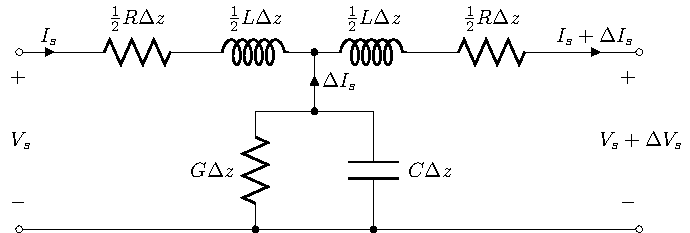
\includegraphics{figTransmissionBaicLines}
\caption{یکساں ترسیلی تار کا چھوٹا حصہ۔ متغیرات $R$، $L$، $C$ اور $G$ تار کی شکل اور مادوں پر منحصر ہیں۔}
\label{شکل_ترسیل_سادہ_نظام}
\end{figure}

یہاں بھی ہم موج کی حرکت \عددیء{\az} جانب تصور کرتے ہیں۔یوں تار کی چھوٹی لمبائی \عددیء{\Delta z} کی مزاحمت \عددیء{R \Delta z}، امالہ \عددیء{L \Delta z}، برقی گنجائش \عددیء{C \Delta z} اور ایصالیت \عددیء{G \Delta z} ہوں گے۔شکل \حوالہ{شکل_ترسیل_سادہ_نظام} میں ترسیلی تار کی اس چھوٹی لمبائی کو دکھایا گیا ہے۔چونکہ تار کا یہ چھوٹا ٹکڑا دونوں اطراف سے بالکل ایک جیسا معلوم ہوتا ہے  لہٰذا اس کے سلسلہ وار اجزاء کو آدھے آدھے ٹکڑوں میں کرتے ہوئے متوازی اجزاء کے دونوں طرف دکھایا گیا ہے۔ہم متوازی اجزاء کو دو برابر ٹکڑوں میں کرتے ہوئے سلسلہ وار اجزاء کے دونوں جانب بھی جوڑ سکتے تھے۔

ہم فرض کرتے ہیں کہ شکل \حوالہ{شکل_ترسیل_سادہ_نظام} میں بائیں طرف برقی دباو
\begin{align*}
V=V_0 \cos (\omega t -\beta z +\psi)
\end{align*}
پایا جاتا ہے۔یہ حرکت کرتی موج کی عمومی مساوات ہے۔یولر\فرہنگ{یولر مماثل}\فرہنگ{Euler's identity} مماثل استعمال کرتے ہوئے اس مساوات کو
\begin{align*}
V=\left[ V_0 e^{j(\omega t -\beta z +\psi)}\right]_{\text{حقیقی}}
\end{align*}
لکھی جا سکتی ہے۔اس مساوات میں \عددیء{e^{j\omega t}} اور زیر نوشت میں \عددیء{_\text{حقیقی}} کو پوشیدہ رکھتے ہوئے دوری سمتیہ کی صورت میں یوں لکھا جا سکتا ہے
\begin{align*}
V_s =V_0 e^{j \psi} e^{-\beta z}
\end{align*}
جہاں مساوات کے بائیں ہاتھ \عددیء{V_s} لکھتے ہوئے زیر نوشت میں \عددیء{s} یاد دلاتی ہے کہ یہ مساوات دوری سمتیہ کی شکل میں ہے۔ 

شکل \حوالہ{شکل_ترسیل_سادہ_نظام} کے گرد گھومتے ہوئے کرخوف کے برقی دباو کے قانون سے
\begin{align*}
V_s=\left(\frac{R\Delta z}{2} + j \frac{\omega L \Delta z}{2}\right) I_s+\left(\frac{R\Delta z}{2} + j \frac{\omega L \Delta z}{2}\right) \left(I_s+\Delta I_s \right)+V_s+\Delta V_s
\end{align*}
یا
\begin{align*}
\frac{\Delta V_s}{\Delta z} =-\left(R+j\omega L \right) I_s-\frac{1}{2}\left(R+j\omega L \right)\Delta I_s
\end{align*}
لکھا جا سکتا ہے۔اگر \عددیء{\Delta z} کو صفر کے قریب تر کیا جائے تب \عددیء{\Delta I_s} بھی صفر کے قریب تر ہو گا۔یوں \عددیء{\Delta z \to 0 } کی صورت میں اس مساوات کے آخری جزو کو نظر انداز کیا جا سکتا ہے۔یوں اسے
\begin{align}\label{مساوات_ترسیل_دباو_تفرقی_مساوات}
\frac{\dif V_s}{\dif z}=-\left(R+j\omega L \right) I_s
\end{align}
لکھا جا سکتا ہے۔

متوازی اجزاء پر برقی دباو
\begin{align*}
V_s-\left(\frac{R \Delta z}{2}+j\frac{\omega L \Delta z}{2} \right) I_s
\end{align*}
ہے جسے استعمال کرتے ہوئے شکل کو دیکھ کر متوازی اجزاء میں تفرقی رو کے لئے
\begin{align*}
-\Delta I_s = \left[V_s-\left(\frac{R \Delta z}{2}+j\frac{\omega L \Delta z}{2} \right) I_s \right] \left(G \Delta z+j \omega C \Delta z \right)
\end{align*}
یا
\begin{align*}
\frac{\Delta I_s}{\Delta z}=-\left(G+j \omega C \right) V_s +\frac{1}{2}\left(R+j \omega L \right)\left(G+j \omega C \right) I_s \Delta z
\end{align*}
لکھا جا سکتا ہے۔ اگر \عددیء{\Delta z \to 0} کیا جائے تب اس مساوات کے آخری جزو کو نظر انداز کیا جا سکتا ہے اور یوں
\begin{align}\label{مساوات_ترسیل_رو_تفرقی_مساوات}
\frac{\dif I_s}{\dif z}=-\left(G+j \omega C \right) V_s
\end{align}
 حاصل ہوتا ہے۔

یہاں رک کر ذرا برقناطیسی امواج کی مساوات کو دوبارہ پیش کرتے ہیں۔میکس ویل کی مساوات
\begin{align*}
\nabla \times \kvec{E}_s=-j \omega \mu \kvec{H}_s
\end{align*}
میں \عددیء{\kvec{E}_s=E_{xs}\ax} اور \عددیء{\kvec{H}_{ys}=H_{ys}\ay}  پر کرنے سے
\begin{align}\label{مساوات_ترسیل_برقی_شدت_تفرقی_مساوات}
\frac{\dif E_{xs}}{\dif z}=-j \omega \mu H_{ys}
\end{align}
ملتا ہے اور اسی طرح
\begin{align*}
\nabla \times \kvec{H}_s=\left(\sigma+j\omega \epsilon \right)\kvec{E}_s
\end{align*}
سے
\begin{align}\label{مساوات_ترسیل_مقناطیسی_شدت_تفرقی_مساوات}
\frac{\dif H_{ys}}{\dif z}=-\left(\sigma+j \omega \epsilon \right) E_{xs}
\end{align}
ملتا ہے۔

مساوات \حوالہ{مساوات_ترسیل_رو_تفرقی_مساوات} کا مساوات \حوالہ{مساوات_ترسیل_مقناطیسی_شدت_تفرقی_مساوات} کے ساتھ موازنہ کریں۔غور کرنے سے معلوم ہوتا ہے کہ پہلی مساوات میں \عددیء{I_s} کی جگہ \عددیء{H_{ys}} لکھنے اور اسی طرح \عددیء{G} کی جگہ \عددیء{\sigma}، \عددیء{C} کی جگہ \عددیء{\epsilon} اور \عددیء{V_s} کی جگہ \عددیء{E_{xs}} لکھتے ہوئے دوسری مساوات حاصل کی جا سکتی ہے۔دونوں مساوات بہت قریبی مشابہت رکھتی ہیں۔

اسی طرح مساوات \حوالہ{مساوات_ترسیل_دباو_تفرقی_مساوات} اور مساوات \حوالہ{مساوات_ترسیل_برقی_شدت_تفرقی_مساوات} کو دیکھتے ہوئے  یہی جوڑے یہاں بھی پائے جاتے ہیں، البتہ یہاں \عددیء{L} اور \عددیء{\mu} کی جوڑی بھی پائی جاتی ہے۔ہاں ظاہری طور پر \عددیء{R} کی جوڑی موجود نہیں ہے۔یوں ہم \عددیء{j \omega \mu} کی جوڑی \عددیء{R+j\omega L} لے سکتے ہیں۔

لامحدود یکساں مستوی امواج اور لامحدود لمبائی کی یکساں ترسیلی تار کی سرحدی شرائط ایک جیسی ہیں۔دونوں میں سرحد پائی ہی نہیں جاتا لہٰذا  ہم گزشتہ باب میں حاصل حل
\begin{align*}
E_{xs}=E_{x0} e^{- \gamma z}
\end{align*}
کی طرز پر اب
\begin{align}
V_s=V_0 e^{- \gamma z}
\end{align}
بطور ترسیلی تار کی مساوات کا حل لکھ سکتے ہیں۔یہ برقی دباو کی موج\فرہنگ{موج!برقی دباو}\فرہنگ{wave!voltage} کی مساوات ہے۔یہ موج مثبت \عددیء{z} جانب حرکت کر رہی ہے اور \عددیء{z=0} پر اس کا حیطہ \عددیء{V_0} ہے۔مساوات \حوالہ{مساوات_موج_حرکی_مستقل_الف} میں دیا گیا حرکی مستقل\فرہنگ{حرکی مستقل}\فرہنگ{propagation constant}
\begin{align*}
\gamma=\sqrt{j \omega \mu (\sigma +j\omega \epsilon)}
\end{align*}
ترسیلی تار کے لئے
\begin{align}
\gamma=\alpha+j\beta=\sqrt{(R+j\omega L)(G+j\omega C)}
\end{align}
لکھا جائے گا۔طول موج\فرہنگ{طول موج}\فرہنگ{موج!طول}\فرہنگ{wavelength} اب بھی
\begin{align}
\lambda=\frac{2\pi}{\beta}
\end{align}
ہو گی۔موج کی رفتار\فرہنگ{موج!رفتار}\فرہنگ{رفتار!موج}\فرہنگ{phase velocity} اب بھی
\begin{align}
v=\frac{\omega}{\beta}
\end{align}
ہے۔

کامل ترسیلی تار طاقت ضائع نہیں کرتی۔ایسی تار کے مستقل \عددیء{R=G=0} ہوتے ہیں لہٰذا
\begin{align*}
\gamma=j \beta=j \omega \sqrt{LC}
\end{align*}
اور 
\begin{align}
v=\frac{1}{\sqrt{LC}}
\end{align}
ہوں گے۔

اسی طرح مقناطیسی موج
\begin{align*}
H_{ys}=\frac{E_{x0}}{Z_0} e^{-\gamma z}
\end{align*}
سے
\begin{align}
I_s=\frac{V_0}{Z_0} e^{-\gamma z}
\end{align}
لکھا جا سکتی ہے۔ترسیلی تار کی قدرتی رکاوٹ\فرہنگ{قدرتی رکاوٹ}\فرہنگ{intrinsic impedance} \عددیء{Z_0} کو مستوی موج کی قدرتی رکاوٹ یعنی مساوات \حوالہ{مساوات-موج_قدرتی_رکاوٹ}
\begin{align*}
Z=\sqrt{\frac{j\omega \mu}{\sigma +j\omega \epsilon}}
\end{align*}
سے
\begin{align}
Z_0=\sqrt{\frac{R+j\omega L}{G+j \omega C}}
\end{align}
لکھا جا سکتا ہے۔

خطہ-1 میں آمدی موج جب خطہ-2 کی سرحد سے ٹکراتی ہے تو اس کا کچھ حصہ بطور انعکاسی موج خطہ-1 میں واپس ہو جاتا ہے۔اس انعکاسی موج اور آمدی موج کی شرح کو شرح انعکاس\فرہنگ{شرح!انعکاس}\فرہنگ{reflection coefficient} کہتے ہیں۔مستوی موج کی شرح انعکاس مساوات \حوالہ{مساوات_موج_شرح_انعکاس_تعریف}
\begin{align*}
\Gamma=\frac{E_{x0}^-}{E_{x0}^+}=\frac{Z_2-Z_1}{Z_2+Z_1}
\end{align*}
دیتی ہے۔اسی طرح اگر \عددیء{Z_{01}} قدرتی رکاوٹ کی ترسیلی تار پر آمد موج \عددیء{Z_{02}} قدرتی رکاوٹ کی ترسیلی تار میں داخل ہونا چاہے تو ان کی سرحد سے انعکاسی موج واپس ہو گی۔ایسی انعکاسی موج اور آمدی موج کی شرح
\begin{align}
\Gamma=\frac{V_0^-}{V_0^+}=\frac{Z_{02}-Z_{01}}{Z_{02}+Z_{01}}
\end{align}
 ہو گی۔انعکاسی شرح جانتے ہوئے شرح ساکن موج\فرہنگ{شرح!ساکن موج}\فرہنگ{standing wave ratio}
\begin{align}
s=\frac{1+\abs{\Gamma}}{1-\abs{\Gamma}}
\end{align}
لکھی جا سکتی ہے۔آخر میں اگر \عددیء{z>0} پر \عددیء{Z=Z_2} ہو تب \عددیء{z=-l} پر \عددیء{E_{xs}} اور \عددیء{H_{ys}} کی شرح 
\begin{align*}
Z_{\text{داخلی}}=Z_1 \frac{Z_2+j Z_1 \tan \beta_1 l}{Z_1 +j Z_2 \tan \beta_1 l}
\end{align*}
کو داخلی قدرتی رکاوٹ  کہتے ہیں۔اس سے \عددیء{z>0} پر \عددیء{Z_{02}} کی صورت میں ترسیلی تار کے لئے \عددیء{z=-l} پر \عددیء{V_s} اور \عددیء{I_s} کی شرح، یعنی اس کی داخلی قدرتی رکاوٹ\فرہنگ{داخلی قدرتی رکاوٹ}\فرہنگ{رکاوٹ!داخلی قدرتی}\فرہنگ{input intrinsic impedance} کو
\begin{align}\label{مساوات_ترسیلی_داخلی_قدرتی_رکاوٹ_تعریف}
Z_{\text{داخلی}}=Z_{01} \frac{Z_{02}+j Z_{01}\tan \beta_1 l}{Z_{01}+j Z_{02}\tan \beta_1 l}
\end{align}
لکھا جا سکتا ہے۔یہاں سے ہم غیر ضروری علامت لکھنے سے گریز کرتے ہوئے \عددی{Z_{01}} کو عموماً \عددی{Z_1} اور \عددی{Z_{02}} کو عموماً \عددی{Z_2} لکھیں گے۔


محدود لمبائی کی ترسیلی تار میں لمحہ \عددی{t=0} پر داخلی سرے سے اختتامی سرے کی جانب  امواج روانہ ہوتی ہیں۔ان امواج کا کچھ حصہ اختتامی سرے پر نسب برقی بوجھ سے انعکاس پذیر ہو کر واپس لوٹے گا۔ اب تار میں آمدی موج کے ساتھ ساتھ انعکاسی امواج بھی پائی جائیں گی۔انعکاسی موج ترسیلی تار کے داخلی سرے پر پہنچ کر یہاں سے منعکس ہوں گی۔یوں تار میں اب اصل آمدی موج کے ساتھ ساتھ دو مرتبہ انعکاس پذیر امواج بھی اختتامی جانب رواں ہوں گی۔ آپ دیکھ سکتے ہیں کہ جلد ہی ترسیلی تار کے دونوں سروں سے بار بار منعکس، لامحدود تعداد کی امواج تار میں پائی جائیں گی۔بجائے یہ کہ ہم تار میں ہر موج پر نظر رکھیں، ہم داخلی جانب سے اختتامی جانب رواں تمام امواج کے مجموعے کو آمدی موج تصور کرتے ہیں۔اسی طرح اختتامی جانب سے داخلی جانب تمام امواج کے مجموعے کو انعکاسی موج تصور کیا جاتا ہے۔ایسا ہی تصور کرتے ہوئے  مساوات \حوالہ{مساوات_ترسیلی_داخلی_قدرتی_رکاوٹ_تعریف} حاصل کیا گیا ہے۔  
%============================
\ابتدا{مشق}
ایک ترسیلی تار  کے مستقل \عددیء{R=\SI{0.15}{\ohm\per\meter}}، \عددیء{L=\SI{0.25}{\micro\henry\per\meter}}، \عددیء{G=\SI{8}{\micro\siemens\per\meter}} اور \عددیء{C=\SI{80}{\pico\farad\per\meter}} ہیں۔ تعدد \عددیء{\omega=\SI{5e8}{\radian\per \second}} پر \عددیء{\alpha}، \عددیء{\beta}، \عددیء{\lambda}، \عددیء{v} اور \عددیء{Z_0} حاصل کریں۔

جوابات: \عددیء{\SI{1.57}{\neper\per\meter}}، \عددیء{\SI{2.236}{\radian\per\meter}}، \عددیء{\SI{2.81}{\meter}}، \عددیء{\SI{2.23e8}{\meter\per\second}} اور  \عددیء{55.9\phase{-0.029^\circ}\, \si{\ohm}}
\انتہا{مشق}
%========================

\حصہ{ترسیلی تار کے مستقل}
اس حصے میں مختلف اشکال کی ترسیلی تار کے مستقل یکجا کرتے ہیں۔ان میں سے عموماً مستقل کو ہم پہلے حاصل کر چکے ہیں، بس انہیں ایک جگہ لکھنا باقی ہو گا۔سب سے پہلے ہم محوری تار کے مستقل اکٹھے کرتے ہیں۔

\begin{figure}
\centering
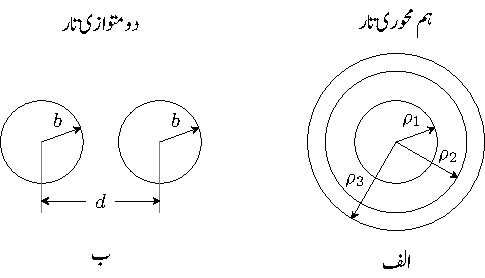
\includegraphics{figTransmissionDifferentLines}
\caption{ہم محوری ترسیلی تار اور دو متوازی ترسیلی تار۔}
\label{شکل_ترسیل_مختلف_ترسیلی_تار}
\end{figure}
\جزوحصہ{ہم محوری تار کے مستقل}
شکل \حوالہ{شکل_ترسیل_مختلف_ترسیلی_تار}-الف میں ہم محوری تار دکھائی گئی ہے جس میں اندرونی تار کا رداس \عددیء{\rho_1} ہے۔بیرونی تار کا اندرونی رداس \عددیء{\rho_2} اور اس کا بیرونی رداس \عددیء{\rho_3} ہیں۔تاروں کے درمیان ذو برق کے مستقل \عددیء{\epsilon}،  \عددیء{\mu} اور \عددیء{\sigma} ہیں۔ صفحہ \حوالہصفحہ{مساوات_کپیسٹر_کپیسٹر_ہم_محوری_تار} پر مساوات میں تار کی لمبائی \عددیء{L=\SI{1}{\meter}} پر کرنے سے اس کی فی میٹر برقی گنجائش
 \begin{align}
C=\frac{Q}{V}=\frac{2\pi\epsilon }{\ln \frac{\rho_2}{\rho_1}}
\end{align}
حاصل ہوتی ہے جبکہ فی میٹر امالہ صفحہ \حوالہصفحہ{مساوات_امالہ_ہم_محوری_کم_تعددی_امالہ} پر مساوات \حوالہ{مساوات_امالہ_ہم_محوری_کم_تعددی_امالہ} دیتی ہے۔
\begin{align}
L_{\text{بیرونی}}=\frac{\mu  I }{2\pi} \ln \frac{\rho_2}{\rho_1}
\end{align}
یہ تار کی بیرونی امالہ ہے۔بلند تعدد پر تار میں برقی رو صرف گہرائی جلد تک محدود رہتی ہے لہٰذا ایسی صورت میں تار کے اندر نہایت کم مقناطیسی بہاو پایا جاتا ہے اور یوں اس کی  اندرونی امالہ قابل نظرانداز ہوتی ہے۔کسی بھی ترسیلی تار کے لئے
\begin{align}\label{مساوات_ترسیلی_امالہ_کپیسٹنس_عمومی_تعلق}
L_{\text{بیرونی}} C=\mu \epsilon
\end{align}
درست ثابت ہوتا ہے۔یوں دونوں ہم محوری تاروں کے درمیان  میں بھری ذو برق کا \عددیء{\epsilon} اور فی میٹر تار کی برقی گنجائش جانتے ہوئے اندرونی امالہ اس مساوات سے حاصل کی جا سکتی ہے۔

کم تعدد پر تار کی اندرونی امالہ کو نظرانداز نہیں کیا جا سکتا۔ایسی صورت میں مساوات \حوالہ{مساوات_امالہ_ہم_محوری_کم_تعددی_فی_میٹر_کل_امالہ}
\begin{align}\label{مساوات_ترسیلی_کم_تعددی_امالہ}
L=\frac{\mu  I }{2\pi} \ln \frac{\rho_2}{\rho_1}+\frac{\mu }{8\pi}+\frac{\mu}{2\pi \left(\rho_3^2-\rho_2^2\right)^2}\left(\rho_3^4 \ln \frac{\rho_3}{\rho_2}-\frac{\rho_2^4}{4}-\frac{3\rho_3^4}{4}+\rho_2^2 \rho_3^2\right)
\end{align}
میں دی گئی فی میٹر تار کی امالہ استعمال کی جائے گی۔یاد رہے کہ یہ امالہ حاصل کرتے ہوئے فرض کیا گیا تھا کہ برقی رو یکساں موصل تار میں گزرتی ہے۔اب ہم جانتے ہیں کہ بلند تعدد پر رو صرف گہرائی جلد تک محدود رہتی ہے لہٰذا کم تعدد پر ہی اس امالہ کو استعمال کیا جا سکتا ہے۔

آئیں ایسی تعدد پر بھی صورت حال دیکھیں جب اندرونی امالہ کی قیمت قابل نظرانداز نہ ہو لیکن گہرائی جلد کے اثر کو بھی نظرانداز نہیں کیا جا سکتا۔ گہرائی جلد کے اثر کی وجہ سے مساوات \حوالہ{مساوات_ترسیلی_کم_تعددی_امالہ} قابل قبول نہیں ہو گی۔اب فرض کرتے ہیں کہ گہرائی جلد \عددیء{\delta} اندرونی تار کے رداس \عددیء{\rho_1} سے بہت کم ہے۔یوں اندرونی تار کے بیرونی باریک تہہ میں برقی رو پائی جائے گی۔برقی رو \عددیء{\az} سمت میں ہے اور چونکہ \عددیء{\kvec{J}_s=\sigma_c \kvec{E}_s} ہوتا ہے لہٰذا تار کی سطح پر \عددیء{\kvec{E}_s} کا مماثل جزو بھی \عددیء{\ax} سمت میں ہو گا۔موصل تار کی موصلیت کو یہاں \عددیء{\sigma_c} لکھا گیا ہے۔ مقناطیسی میدان کی شدت تار کی سطح پر 
\begin{align}\label{مساوات_ترسیلی_ہم_محوری_تار_اندرونی_تار_مقناطیسی_میدان}
H_{\phi s}=\frac{I_s}{2\pi \rho_1}
\end{align}
ہو گی۔اب تار کی سطح پر \عددیء{E_{zs}} اور \عددیء{H_{ys}} کی شرح، مستوی برقناطیسی موج کی  قدرتی رکاوٹ ہو گی۔اگرچہ ہم نلکی اشکال کی بات کر رہے ہیں لیکن \عددیء{\delta \ll \rho_1} کی بنا پر برقی رو گزارتے باریک تہہ کو \عددیء{\delta} موٹائی اور \عددیء{2\pi \rho_1} چوڑائی کا موصل تصور کیا جا سکتا ہے۔یوں صفحہ \حوالہصفحہ{مساوات_موج_قدرتی_رکاوٹ_موصل_گہرائی_جلد_کے_ساتھ} پر مساوات \حوالہ{مساوات_موج_قدرتی_رکاوٹ_موصل_گہرائی_جلد_کے_ساتھ} سے
\begin{align*}
\left. \frac{E_{zs}}{H_{ys}}\right|_{\rho_1}=\frac{1+j}{\sigma_c \delta}
\end{align*}
لکھا جا سکتا ہے جس میں مساوات \حوالہ{مساوات_ترسیلی_ہم_محوری_تار_اندرونی_تار_مقناطیسی_میدان} پر کرنے سے
\begin{align*}
\left. \frac{E_{zs}}{I_s} \right|_{\rho_1} =\frac{1+j}{2\pi \rho_1 \delta \sigma_c }
\end{align*}
لکھا جا سکتا ہے۔چونکہ \عددیء{E_{zs}} دراصل فی میٹر برقی دباو ہے لہٰذا مندرجہ بالا شرح فی میٹر قدرتی رکاوٹ
\begin{align}\label{مساوات_ترسیلی_رکاوٹ_بلند_تعدد_ہم_محوری}
Z=\left. \frac{E_{zs}}{I_s} \right|_{\rho_1}=R+j \omega L=\frac{1}{2\pi \rho_1 \delta \sigma_c }+j \frac{1}{2\pi \rho_1 \delta \sigma_c }
\end{align}
 کے برابر ہے۔یہ امالہ تار کی اندرونی امالہ ہے جو تار کی موصلیت \عددیء{\sigma_c} پر منحصر ہے۔آپ دیکھ سکتے ہیں کہ کامل موصل کی صورت میں قدرتی رکاوٹ صفر ہو گی۔یوں اندرونی تار کی اندرونی امالہ
\begin{align*}
L_{\rho_1,\text{اندرونی}}=\frac{1}{2\pi \rho_1 \delta \sigma_c \omega}
\end{align*}
ہو گی۔صفحہ \حوالہصفحہ{مساوات_موج_گہرائی_جلد_تعریف} پر مساوات \حوالہ{مساوات_موج_گہرائی_جلد_تعریف} کو \عددیء{\sigma_c=\tfrac{1}{\pi f \mu \delta^2}} لکھتے ہوئے اس میں پر کرنے سے
\begin{align}
L_{\rho_1,\text{اندرونی}}=\frac{\mu \delta}{4 \pi \rho_1} \quad (\delta \ll \rho_1)
\end{align}
حاصل ہوتا ہے۔اسی طریقہ کار سے بیرونی تار کے لئے
\begin{align}
L_{\rho_2,\text{اندرونی}}=\frac{\mu \delta}{4 \pi \rho_2} \quad (\delta \ll \rho_3-\rho_2)
\end{align}
لکھا جا سکتا ہے۔یوں بلند تعدد پر ہم محوری تار کی کل امالہ
\begin{align}
L_{\text{\RL{بلند تعدد}}}=\frac{\mu }{2 \pi }   \left[\ln \frac{\rho_2}{\rho_1} +\frac{\sigma_c}{2} \left(\frac{1}{\rho_1}+\frac{1}{\rho_2} \right)\right] \quad (\delta \ll \rho_1, \, \delta \ll \rho_3-\rho_2)
\end{align}
ہو گی۔مساوات \حوالہ{مساوات_ترسیلی_رکاوٹ_بلند_تعدد_ہم_محوری} بلند تعدد پر قدرتی رکاوٹ کا مزاحمتی حصہ یعنی فی میٹر مزاحمت بھی دیتا ہے جس سے  اندرونی اور بیرونی تاروں کا سلسلہ وار مجموعہ
\begin{align}
R=\frac{1}{2\pi \delta \sigma_c} \left(\frac{1}{\rho_1}+\frac{1}{\rho_2} \right) \quad (\delta \ll \rho_1, \,  \delta \ll \rho_3-\rho_2)
\end{align}
لکھا جا سکتا ہے۔اس مزاحمت کے ساتھ شعاعی اخراج سے پیدا مزاحمتی جزو بھی شامل کیا جا سکتا ہے۔\اصطلاح{بے پردہ}\فرہنگ{بے پردہ}\حاشیہب{unshielded}\فرہنگ{unshielded} تار یا ہم محوری تار کے کھلے سر سے شعاعی اخراج ہوتا ہے۔ 

ایسی تعدد جس پر گہرائی جلد کی قیمت رداس سے بہت کم نہ ہو حل کرتے ہوئے \اصطلاح{بیسل تفاعل}\فرہنگ{بیسل تفاعل}\حاشیہب{Bessel functions}\فرہنگ{Bessel functions} استعمال ہوتے ہیں۔یہاں انہیں حل نہیں کیا جائے گا۔

قدرتی رکاوٹ کو عموماً بیرونی امالہ اور برقی گنجائش  کی صورت میں
\begin{align}
Z_0=\sqrt{\frac{L_{\text{بیرونی}}}{C}} =\frac{1}{2\pi} \sqrt{\frac{\mu}{\epsilon}} \ln \frac{\rho_2}{\rho_1}
\end{align}
لکھا جاتا ہے۔ 

اندرونی اور بیرونی تار کے مابین ذو برق میں سے گزرتی یک سمت برقی رو \عددیء{I=G V} سے حاصل ہوتی ہے۔اندرونی تار پر \عددیء{\rho_L} اور بیرونی تار پر \عددیء{-\rho_L} کثافت لکیری بار تصور کرتے ہوئے تاروں کے مابین برقی دباو صفحہ \حوالہصفحہ{مساوات_توانائی_ہم_محوری_تار_برقی_دباو} پر مساوات \حوالہ{مساوات_توانائی_ہم_محوری_تار_برقی_دباو}
\begin{align*}
V=\frac{\rho_L}{2\pi \epsilon} \ln \frac{\rho_2}{\rho_1}
\end{align*}
دیتی ہے۔تاروں کے درمیان ذو برق میں میدان مساوات \حوالہ{مساوات_توانائی_ہم_محوری_تار_ذوبرق_میدان}
\begin{align*}
E_{\rho}=\frac{\rho_L}{2\pi \epsilon \rho}
\end{align*}
دیتی ہے۔ ذو برق کی موصلیت \عددیء{\sigma} لکھتے ہوئے، صفحہ \حوالہصفحہ{مساوات_کپیسٹر-اوہم_قانون_نقطہ_شکل} پر اوہم کے قانون کی نقطہ شکل یعنی مساوات \حوالہ{مساوات_کپیسٹر-اوہم_قانون_نقطہ_شکل} کی مدد سے یوں رداس \عددیء{\rho} پر کثافت  برقی رو
\begin{align*}
J_{\rho}=\sigma E_{\rho}=\frac{\sigma \rho_L}{2\pi \epsilon \rho}
\end{align*}
لکھی جائے گی۔اندرونی تار کے گرد رداس \عددیء{\rho} پر \عددیء{L} لمبائی کی نلکی سطح کا رقبہ \عددیء{2\pi \rho L} ہو گا۔ایسی اکائی لمبائی کی سطح کے رقبہ 
\عددیء{2\pi \rho }  سے کل
\begin{align*}
I= J_{\rho} 2\pi \rho=\frac{\sigma \rho_L}{\epsilon}
\end{align*}
برقی رو گزرے گی۔یوں
\begin{align}
G=\frac{I}{V}=\frac{2\pi \sigma}{\ln \frac{\rho_2}{\rho_1}}
\end{align}
حاصل ہوتا ہے۔

یہاں \عددیء{G} کی قیمت \عددیء{C} کی قیمت سے حاصل کرنا دیکھتے ہیں۔ایک تار سے دوسرے تار تک \عددیء{\kvec{E}} کی لکیری تکمل سے برقی دباو \عددیء{V} حاصل ہوتا ہے۔صفحہ \حوالہصفحہ{مساوات_کپیسٹر_عمودی_میدان_برابر_کثافت_بار} پر مساوات \حوالہ{مساوات_کپیسٹر_عمودی_میدان_برابر_کثافت_بار} کے تحت کسی بھی موصل پر سطحی کثافت بار، سطح کے عمودی برقی بہاو کے برابر ہوتی ہے، یعنی \عددیء{\rho_S=D_{\text{عمودی}}}۔یوں تار پر کل بار
\begin{align*}
Q=\int_S \rho_S \dif S = \epsilon \int_S E_{\text{عمودی}} \dif S
\end{align*}
لکھی جا سکتی ہے جہاں \عددیء{S} تار کا سطحی رقبہ ہے اور \عددیء{D=\epsilon E} لکھا گیا گا۔یوں
\begin{align}\label{مساوات_ترسیلی_ہم_محوری_تار_کپیسٹنس_عمومی_مساوات}
C=\frac{Q}{V}=\frac{\epsilon \int_S E_{\text{عمودی}} \dif S}{V}
\end{align}
ہو گا۔اب موصل کی سطح پر \عددیء{E_{\text{عمودی}}} جانتے ہوئے یہاں کثافت برقی رو \عددیء{J=\sigma E_{\text{عمودی}}} لکھی جا سکتی ہے لہٰذا تار کے سطح سے خارج کل برقی رو
\begin{align*}
I=\sigma \int_S E_{\text{عمودی}} \dif S
\end{align*}
ہو گی۔یوں دو تاروں کے مابین ایصالیت
\begin{align}\label{مساوات_ترسیلی_ہم_محوری_تار_ایصالیت_عمومی_مساوات}
G=\frac{I}{V}=\frac{\sigma \int_S E_{\text{عمودی}} \dif S}{V}
\end{align}
ہو گی۔مساوات \حوالہ{مساوات_ترسیلی_ہم_محوری_تار_کپیسٹنس_عمومی_مساوات} اور مساوات \حوالہ{مساوات_ترسیلی_ہم_محوری_تار_ایصالیت_عمومی_مساوات} کو دیکھ کر
\begin{align}\label{مساوات_ترسیلی_کپیسٹنس_ایصالیت_تعلق}
G=\frac{\sigma}{\epsilon} C
\end{align}
لکھا جا سکتا ہے جو کسی بھی ترسیلی تار کے لئے درست ہے
%=====================
\ابتدا{مشق}
ایک ہم محوری تار جس کے \عددیء{\rho_1=\SI{1}{\milli\meter}}،  \عددیء{\rho_2=\SI{3.49}{\milli \meter}} اور \عددیء{\sigma_c=\SI{3.82e7}{\siemens\per\meter}} ہیں کے ذو برق کے مستقل \عددیء{\mu_R=1}، \عددیء{\epsilon_R=2.25} اور \عددیء{\sigma=\SI{10}{\micro \siemens \per \meter}} ہیں۔ اس کی فی میٹر برقی گنجائش، بیرونی اور اندرونی امالہ حاصل کریں۔ترسیلی تار کے \عددیء{\alpha}، \عددیء{\beta} اور \عددیء{Z_0} بھی حاصل کریں۔

جوابات: \عددیء{\SI{0.1}{\nano\farad\per\meter}}، \عددیء{\SI{0.25}{\micro\henry\per\meter}}، \عددیء{\SI{1.29}{\nano\henry\per\meter}}،  \عددیء{\SI{0.014}{\neper\per\meter}}، \عددیء{\SI{15.1}{\radian\per\meter}} اور
  \عددیء{50\phase{0.055^\circ} \, \si{\ohm}}
\انتہا{مشق}
%====================
\جزوحصہ{دو متوازی تار کے مستقل}
شکل \حوالہ{شکل_ترسیل_مختلف_ترسیلی_تار}-ب میں دو متوازی ترسیلی تار دکھائی گئی ہے۔تار کا رداس \عددیء{b}، تاروں کے مابین فاصلہ \عددیء{d} جبکہ تار کی موصلیت \عددیء{\sigma_c} ہے۔تاروں کے گرد ذو برق کے مستقل \عددیء{\epsilon}،  \عددیء{\mu} اور \عددیء{\sigma} ہیں۔ اس تار کی برقی گنجائش صفحہ \حوالہصفحہ{مساوات_کپیسٹر_نلکی_زمین_کپیسٹنس} پر مساوات \حوالہ{مساوات_کپیسٹر_نلکی_زمین_کپیسٹنس} کی نصف ہو گی۔اس کی وجہ وہیں پر مساوات کے نیچے سمجھائی گئی ہے۔یوں فی میٹر تار کی برقی گنجائش
\begin{align}
C=\frac{\pi\epsilon }{\cosh^{-1} \frac{d}{2 b}}
\end{align}
ہو گی۔اگر \عددیء{b\ll d} ہو تب مساوات \حوالہ{مساوات_کپیسٹر_نلکی_زمین_کپیسٹنس_ب} سے
\begin{align*}
C=\frac{\pi\epsilon }{ \ln \frac{d}{b}} \quad( b \ll d )
\end{align*}
لکھی جا سکتا ہے۔مساوات \حوالہ{مساوات_ترسیلی_امالہ_کپیسٹنس_عمومی_تعلق} سے تار کی فی میٹر بیرونی امالہ
\begin{align*}
L_{\text{بیرونی}}=\frac{\mu}{\pi} \cosh^{-1} \frac{d}{2b}
\end{align*}
یا
\begin{align*}
L_{\text{بیرونی}}=\frac{\mu}{\pi} \ln \frac{d}{b} \quad(b \ll d)
\end{align*}
لکھی جا سکتی ہے جبکہ بلند تعدد پر فی میٹر کل امالہ
\begin{align}
L_{\text{\RL{بلند تعدد}}}=\frac{\mu}{\pi} \left(\frac{\delta}{2b}+\cosh^{-1} \frac{d}{2 b} \right) \quad(\delta \ll b)
\end{align}
ہے۔تار کی بیرونی \عددیء{\delta} تہہ برقی رو گزارتی ہے۔اس تہہ کا رقبہ عمودی تراش \عددیء{S=2\pi b \delta} ہے لہٰذا فی میٹر مزاحمت
\begin{align}
R=\frac{l}{\sigma_c S}=\frac{1}{\pi b \delta \sigma_c}
\end{align}
ہو گی جہاں دونوں تاروں کی مزاحمت سلسلہ وار جڑے ہیں۔مساوات \حوالہ{مساوات_ترسیلی_کپیسٹنس_ایصالیت_تعلق} سے فی میٹر تار کی ایصالیت
\begin{align}
G=\frac{\pi \sigma}{\cosh^{-1} \frac{d}{2b}}
\end{align}
حاصل ہوتی ہے۔

بیرونی امالہ اور برقی گنجائش استعمال کرتے ہوئے قدرتی مزاحمت
\begin{align}
Z_0=\frac{1}{\pi} \sqrt{\frac{\mu}{\epsilon}} \cosh^{-1} \frac{d}{2b}
\end{align}
حاصل ہوتی ہے۔

\begin{figure}
\centering
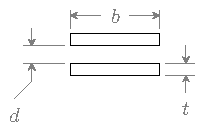
\includegraphics{figTransmissionStripLine}
\caption{سطح مستوی ترسیلی تار۔}
\label{شکل_ترسیلی_سطح_مستوی}
\end{figure}

\جزوحصہ{سطح مستوی ترسیلی تار}
شکل \حوالہ{شکل_ترسیلی_سطح_مستوی} میں \اصطلاح{سطح مستوی ترسیلی تار}\فرہنگ{سطح مستوی ترسیلی تار}\فرہنگ{ترسیلی!سطح مستوی}\حاشیہب{stripline}\فرہنگ{stripline} دکھائی گئی ہے جس میں \عددیء{b} چوڑائی اور \عددیء{t} موٹائی کے دو متوازی موصل چادر دکھائے گئے ہیں جن کے مابین فاصلہ \عددیء{d} ہے۔موصل چادر کی موصلیت \عددیء{\sigma_c} جبکہ اردگرد کے ذو برق کے مستقل \عددیء{\epsilon}، \عددیء{\mu} اور \عددیء{\sigma} ہیں۔

اگر \عددیء{b\gg d} ہو تب ان چادروں کی فی میٹر برقی گنجائش  
\begin{align}
C=\frac{\epsilon \text{رقبہ}}{ \text{فاصلہ}} = \frac{\epsilon b}{d}
\end{align}
ہو گی۔یوں مساوات \حوالہ{مساوات_ترسیلی_امالہ_کپیسٹنس_عمومی_تعلق} سے فی میٹر بیرونی امالہ
\begin{align}
L_{\text{بیرونی}}=\frac{\mu \epsilon}{C}=\frac{\mu d}{b}
\end{align}
ہو گی۔امید کی جاتی ہے کہ آپ گہرائی جلد استعمال کرتے ہوئے اندرونی امالہ حاصل کر سکتے ہیں۔یوں کل امالہ
\begin{align}
L=\frac{\mu d}{b}+\frac{2}{\sigma_c \delta b w}=\frac{\mu}{b} (d+\delta) \quad (\delta \ll t)
\end{align}
ہو گی جہاں گہرائی جلد کو چادر کی موٹائی سے بہت کم تصور کیا گیا ہے۔

بلند تعدد پر برقی رو چادروں کے آمنے سامنے  سطحوں پر گہرائی جلد تک محدود ہو گی۔یوں برقی رو رقبہ \عددیء{b \delta} سے گزرے گی جس سے ایک تار کی اکائی لمبائی کی مزاحمت \عددیء{\tfrac{1}{\sigma_c b \delta}} حاصل ہوتی ہے۔یوں اکائی لمبی تار کے دونوں حصوں کی سلسلہ وار جڑی کل مزاحمت
\begin{align}
R=\frac{2}{\sigma_c b \delta} \quad (\delta \ll t)
\end{align}
ہو گی۔ 

مساوات \حوالہ{مساوات_ترسیلی_کپیسٹنس_ایصالیت_تعلق} سے
\begin{align}
G=\frac{\sigma b}{d}
\end{align}
لکھی جا سکتی ہے۔

ان معلومات سے سطح مستوی ترسیلی تار کی قدرتی رکاوٹ
\begin{align}
Z_0=\sqrt{\frac{L_{\text{بیرونی}}}{C}}=\sqrt{\frac{\mu}{\epsilon}} \frac{d}{b}
\end{align}
لکھی جا سکتی ہے۔
%=======================
\ابتدا{مشق}
مندرجہ بالا تینوں اقسام کے ترسیلی تار \عددیء{\SI{400}{\mega \hertz}} پر کام کر رہے ہیں۔ان میں طاقت کے ضیاع کو نظرانداز کرتے ہوئے تمام کے لئے \عددیء{\lambda} اور \عددیء{\Gamma} حاصل کریں۔ہم محوری تار کا \عددیء{\rho_1=\SI{0.5}{\milli\meter}}، \عددیء{\rho_2=\SI{2.8}{\milli \meter}}، \عددیء{\mu_R=1} اور \عددیء{\epsilon_R=3.1} ہیں۔ متوازی تار کے \عددیء{b=\SI{0.5}{\milli\meter}}، \عددیء{d=\SI{9}{\milli\meter}}، \عددیء{\mu_R=1} اور \عددیء{\epsilon_R=5} ہیں۔ مستوی سطح کے \عددیء{d=\SI{0.2}{\milli\meter}}، \عددیء{b=\SI{5}{\milli\meter}}، \عددیء{\mu_R=1} اور \عددیء{\epsilon_R=2.2} ہیں۔

جوابات: \عددیء{\SI{42.6}{\centi\meter}}، \عددیء{0.26}، \عددیء{\SI{33.5}{\centi\meter}}، \عددیء{-0.215}، \عددیء{\SI{50.6}{\centi\meter}}، \عددیء{0.816}
\انتہا{مشق}
%=====================

\حصہ{ترسیلی تار کی چند مثال}
اس حصے میں گزشتہ حصوں کے نتائج استعمال کرتے ہوئے چند مثال کرتے ہیں۔یہاں تمام ترسیلی تاروں کو بے ضیاع تار تصور کیا جائے گا۔

شروع دو متوازی ترسیلی تار سے کرتے ہیں جس کی قدرتی رکاوٹ \عددیء{\SI{300}{\ohm}} ہے۔ ایسی تار \اصطلاح{ٹی وی}\فرہنگ{ٹی وی}\حاشیہب{TV, television}\فرہنگ{TV} کے اینٹینا اور ٹی وی کے مابین لگائی جاتی ہے۔شکل \حوالہ{شکل_ترسیلی_اینٹینا_تا_ٹی_وی}-الف میں اس طرح جڑے ترسیلی نظام کو دکھایا گیا ہے۔اینٹینا کا تھونن\فرہنگ{تھونن}\حاشیہب{Thevenin}\فرہنگ{Thevenin} مساوی دور استعمال کیا گیا ہے جو ایک عدد منبع برقی دباو \عددیء{V_s} اور اس کے ساتھ سلسلہ وار  جڑی \عددیء{\SI{300}{\ohm}} کی مزاحمت پر مشتمل ہے۔ترسیلی تار ٹی وی کے برقیاتی دور کے بالکل شروع میں نسب ابتدائی ایمپلی فائر سے جڑتی ہے جس کی داخلی مزاحمت \عددیء{\SI{300}{\ohm}} ہے۔ٹی وی کو اسی مزاحمت سے ظاہر کیا گیا ہے۔اس مثال میں ٹی وی بطور برقی بوجھ کردار ادا کرتا ہے۔ٹی وی اسٹیشن سے خارج \عددیء{\SI{100}{\mega \hertz}} کے برقناطیسی امواج اس اینٹینا میں \عددیء{\SI{5}{\milli\volt}} کا اشارہ پیدا کرتی ہیں۔ترسیلی تار کے مستقل ایسے ہیں کہ اس میں اشارات کی رفتار \عددیء{\SI{2.5e8}{\meter\per\second}} ہے۔

\begin{figure}
\centering
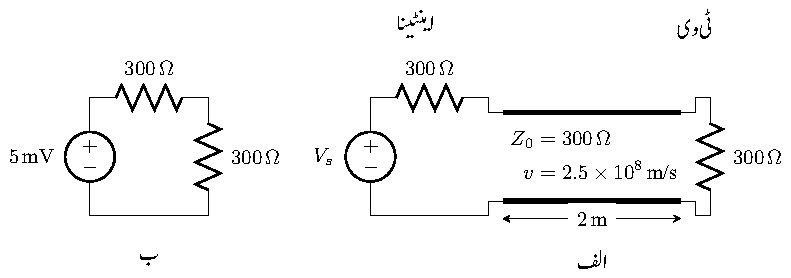
\includegraphics[width=\textwidth]{figTransmissionThreeHundredOhmExample}
\caption{ترسیلی تار اینٹینا کو ٹی وی سے جوڑ رہی ہے۔}
\label{شکل_ترسیلی_اینٹینا_تا_ٹی_وی}
\end{figure}

چونکہ برقی بوجھ کی مزاحمت اور ترسیلی تار کی قدرتی مزاحمت برابر ہیں لہٰذا ترسیلی تار اور برقی بوجھ ہمہ رکاوٹ ہیں۔یوں برقی بوجھ پر انعکاس نہیں پایا جائے گا لہٰذا شرح انعکاس
\begin{align*}
\Gamma=\frac{300-300}{300+300}=0
\end{align*}
 صفر اور شرح ساکن موج
\begin{align*}
s=\frac{1-\abs{\Gamma}}{1+\abs{\Gamma}}=\frac{1-0}{1+0}=1
\end{align*}
ایک کے برابر ہوں گے۔اشارے کے تعدد پر ترسیلی تار میں طول موج
\begin{align*}
\lambda=\frac{v}{f}=\frac{2.5 \times 10^8}{100\times 10^6}=\SI{2.5}{\meter}
\end{align*}
اور زاویائی مستقل
\begin{align*}
\beta=\frac{2\pi}{\lambda}=\frac{2\pi}{2.5}=0.8 \pi\, \si{\radian \per \meter}
\end{align*}
 ہیں۔ترسیلی تار کی برقی لمبائی
\begin{align*}
\beta l =0.8 \pi \times 2=1.6 \pi \, \si{\radian}
\end{align*} 
یا \عددیء{288^\circ} ہے جسے \عددیء{0.8} طول موج بھی کہا جاتا ہے۔ 

شکل \حوالہ{شکل_ترسیلی_اینٹینا_تا_ٹی_وی}-ب میں داخلی جانب کی صورت حال دکھائی گئی ہے۔داخلی جانب چونکہ اینٹینا کی مزاحمت \عددیء{\SI{300}{\ohm}} ہے اور ترسیلی تار کی قدرتی رکاوٹ بھی \عددیء{\SI{300}{\ohm}} ہے لہٰذا  اینٹینا اور ترسیلی تار ہمہ رکاوٹ ہیں۔اینٹینا میں پیدا \عددیء{\SI{5}{\milli \volt}} کا اشارہ ترسیلی تار کی قدرتی رکاوٹ پر 
\begin{align*}
\frac{5 \times 10^{-3} \times 300}{300+300}=\SI{2.5}{\milli \volt}
\end{align*}
پیدا کرے گا۔اینٹینا اور ترسیلی تار ہمہ رکاوٹ ہیں لہٰذا منبع طاقت \عددیء{V_s} ترسیلی تار میں زیادہ سے زیادہ طاقت بھیجے گا۔ترسیلی تار کے داخلی جانب پیدا \عددیء{\SI{2.5}{\milli \volt}} کا اشارہ تار میں سے گزرتے ہوئے برقی بوجھ تک پہنچے گا البتہ یہ داخلی اشارے سے \عددیء{1.6 \pi} ریڈیئن پیچھے ہو گا۔یوں اگر ترسیلی تار کا داخلی اشارہ
\begin{align*}
V_{\text{داخلی}}=2.5 \cos 2\pi 10^8 t \quad \si{\milli \volt}
\end{align*}
ہو تب برقی بوجھ پر اشارہ
\begin{align*}
V_{\text{\RL{بار}}}=2.5 \cos (2\pi 10^8 t-1.6 \pi) \quad \si{\milli \volt}
\end{align*}
ہو گا۔داخلی برقی رو
\begin{align*} 
I_{\text{داخلی}}=\frac{V_{\text{داخلی}}}{300} =8.33 \cos 2\pi 10^8 t \quad \si{\micro \ampere}
\end{align*}
اور برقی بوجھ پر برقی رو
\begin{align*} 
I_{\text{بار}}=\frac{V_{\text{داخلی}}}{300} =8.33 \cos (2\pi 10^8 t -1.6\pi) \quad \si{\micro \ampere}
\end{align*}
ہوں گے۔چونکہ ترسیلی تار بے ضیاع تار ہے لہٰذا جو طاقت اسے داخلی جانب فراہم کی جاتی ہے وہی طاقت خارجی جانب برقی بوجھ کو  مہیا کر دی جاتی ہے۔
\begin{align*}
P_{\text{داخلی}} =P_{\text{بار}}= V_{\text{موثر}} I_{\text{موثر}}=\frac{ 2.5 \times 10^{-3}}{\sqrt{2}} \times \frac{8.33 \times 10^{-6}}{\sqrt{2}}=\SI{10.41}{\nano\watt} 
\end{align*}
مزاحمتی بوجھ کی طاقت کا حساب لگاتے وقت یاد رہے کہ \عددیء{P=VI} میں برقی دباو اور برقی رو کے موثر\فرہنگ{موثر}\حاشیہب{RMS, effective}\فرہنگ{RMS} قیمتیں استعمال کی جاتی ہیں۔سائن نما موج کی موثر قیمت موج کی چوٹی تقسیم \عددیء{\sqrt{2}} کے برابر ہوتی ہے۔

اب پہلے ٹی وی کے متوازی دوسرا ٹی وی نسب کرنے کے اثرات پر غور کرتے ہیں۔دوسرے ٹی وی کی داخلی مزاحمت بھی \عددیء{\SI{300}{\ohm}} ہے۔یوں اب ترسیلی تار کے خارجی جانب کل \عددیء{\SI{150}{\ohm}} کا بوجھ پایا جاتا ہے۔اس طرح شرح انعکاس
\begin{align*}
\Gamma=\frac{150-300}{150=300}=-\frac{1}{3}
\end{align*}
یا
\begin{align}
\Gamma=\frac{1}{3}\phase{\pi}
\end{align}
حاصل ہوتی ہے اور شرح ساکن موج
\begin{align*}
s=\frac{1+\frac{1}{3}}{1-\frac{1}{3}}=2
\end{align*}
ہوں گے۔ترسیلی تار کی داخلی مزاحمت اب \عددیء{\SI{300}{\ohm}} کی بجائے
\begin{align*}
Z_{\text{داخلی}} &=Z_0 \frac{Z_L +j Z_0 \tan \beta l}{Z_0+j Z_L \tan \beta l}=300 \frac{150+j 300 \tan 288^\circ}{300+j 150 \tan 288^\circ}\\
&=509.7 \phase{-23.79^\circ}=466.39-j 205.6 \quad \si{\ohm} 
\end{align*}
ہو گی جو برق گیر (کپیسٹر)  کی خاصیت رکھتی ہے۔برق گیر (کپیسٹر)  کی خاصیت کا مطلب یہ ہے کہ ترسیلی تار کے برقی میدان میں مقناطیسی میدان سے زیادہ توانائی ذخیرہ ہے۔داخلی رو
\begin{align*}
I_{s,\text{داخلی}} &= \frac{0.005}{300+466.39-j 205.6} \\
&=6.3013\phase{15.017^\circ} \quad \si{\micro \ampere}
\end{align*} 
ہے اور یوں ترسیلی تار کو داخلی جانب
\begin{align*}
P_{\text{داخلی}}  &= \frac{1}{2} \left(6.3013 \times 10^{-6} \right)^2 \times 466.39 \\
&= \SI{9.2593}{\nano \watt}
\end{align*}
طاقت فراہم کی جا رہی ہے۔بے ضیاع تار تمام کی تمام طاقت خارجی جانب منتقل کرے گی لہٰذا \عددیء{\SI{150}{\ohm}} کے برقی بوجھ کو \عددیء{\SI{9.2593}{\nano \watt}} حاصل ہو گا جو گزشتہ جواب یعنی \عددیء{\SI{10.41}{\nano\watt} } سے قدر کم ہے۔یہ کمی انعکاس کی وجہ سے پیدا ہوئی۔ کہانی یہاں ختم نہیں ہوتی۔یہ طاقت دونوں ٹی وی میں برابر تقسیم ہو گی لہٰذا ہر ٹی وی کو صرف \عددیء{\SI{4.6297}{\nano\watt} }  طاقت مہیا ہو گا۔چونکہ ایک ٹی وی \عددیء{\SI{300}{\ohm}} مزاحمت رکھتا ہے لہٰذا ٹی وی پر پیدا برقی دباو
\begin{align*}
4.6297 \times 10^{-9} = \frac{\abs{V_{s,\text{\RL{بار}}}}^2}{2 \times 300}
\end{align*}
یعنی
\begin{align*}
\abs{V_{s,\text{\RL{بار}}}}=\SI{1.66667}{\milli \volt}
\end{align*}
ہو گا۔یہ قیمت \عددیء{\SI{2.5}{\milli \volt}} سے بہت کم ہے جو اکیلے ٹی وی پر پیدا ہوتی ہے۔

آئیں ترسیلی تار پر برقی دباو کی چوٹی، نشیب اور ان کے مقامات کے علاوہ دیگر معلومات بھی حاصل کریں۔اگر ہم برقی دباو کی معلومات حاصل کر سکیں تو ظاہر ہے کہ برقی رو کی معلومات بھی حاصل کر پائیں گے۔گزشتہ باب میں مستوی امواج کے لئے یہی معلومات حاصل کی گئیں تھیں۔ وہاں استعمال کی گئی ترکیب یہاں بھی کارآمد ثابت ہوں گی۔برقی دباو موج کے چوٹی کے مقامات مساوات \حوالہ{مساوات_موج_مقام_بلندتر_دباو}
\begin{align*}
-\beta_1 z_{\text{بلندتر}} =\frac{\phi}{2}+ n \pi \quad (n=0,\mp1,\mp 2, \cdots)
\end{align*}
دیتی ہے۔اس میں \عددیء{\beta=0.8 \pi} اور \عددیء{\phi=\pi} پر کرنے سے
\begin{align*}
z_{\text{بلندتر}} &=\frac{1}{-0.8 \pi} \left(\frac{\pi}{2}+n \pi \right)\\
&=-1.25\left(\frac{1}{2}+n \right)
\end{align*}
حاصل ہوتا ہے جس میں \عددیء{n=0}  اور \عددیء{n=1} پر کرنے سے
\begin{align*}
z_{\text{بلندتر}}=  \SI{-0.625}{\meter}  \quad \text{اور} \quad \SI{-1.875}{\meter}
\end{align*}
حاصل ہوتے ہیں جو درست جوابات ہیں۔اگر \عددیء{n=2} پر کیا جائے تو \عددیء{z_{\text{بلندتر}}=\SI{-3.125}{\meter}} حاصل ہوتا ہے جبکہ تار کی کل لمبائی صرف دو میٹر ہے لہٰذا اس جواب کو رد کیا جاتا ہے۔اسی طرح \عددیء{n=-1} پر کرنے سے  \عددیء{z_{\text{بلندتر}}=\SI{+0.625}{\meter}} حاصل ہوتا ہے جبکہ تار منفی \عددیء{z} محدد پر پائی جاتی ہے لہٰذا اس جواب کو بھی رد کیا جاتا ہے۔

موج کی چوٹی سے \عددیء{\tfrac{\lambda}{4}} فاصلے پر نشیب پائے جاتے ہیں، لہٰذا ان کے مقامات
\begin{align*}
z_{\text{کمتر}} = \SI{0}{\meter} \quad \text{اور} \quad \SI{-1.25}{\meter}
\end{align*}
ہوں گے۔آپ نے دیکھا کہ سرحد پر برقی دباو کا نشیب پایا جاتا ہے۔آپ کو یاد ہو گا کہ حقیقی \عددیء{Z_0} اور \عددیء{Z_L} کی صورت میں اگر \عددیء{Z_0<Z_L} ہو تب سرحد پر موج کا نشیب ہی پایا جاتا ہے۔

چونکہ سرحد پر موج کا نشیب ہے اور ہم جانتے ہیں کہ ٹی وی پر \عددیء{\SI{1.66}{\milli \volt}} ہے لہٰذا دباو کی کمتر قیمت یہی ہے اور \عددیء{s=2} سے دباو کی چوٹی اس کے دگنی یعنی \عددیء{\SI{3.32}{\milli\volt}} حاصل ہوتی ہے۔ترسیلی تار کے داخلی سرے پر برقی دباو
\begin{align*}
V_{s,\text{داخلی}} &= I_{s,\text{داخلی}} Z_{\text{داخلی}} \\
&=\left(6.3013 \times 10^{-6}\phase{15.017^\circ} \right)\left(509.7 \phase{-23.79^\circ} \right) \\
&=0.00321175\phase{-8.77^\circ}
\end{align*}
ہو گا جو تقریباً موج کے چوٹی کی برابر ہے۔ایسا اس لئے ہے کہ سرحد سے \عددیء{\tfrac{\lambda}{4}}  فاصلے پر چوٹی پائی جاتی ہے جس سے ہر \عددیء{0.5\lambda} فاصلے پر چوٹی ہو گی لہٰذا سرحد سے \عددیء{\tfrac{3\lambda}{4}} فاصلے پر بھی چوٹی متوقع ہے جو تار کے داخلی سرے کے بہت قریب نقطہ ہے۔آپ ترسیلی تار کی داخلی برقی دباو یوں
\begin{align*}
V_{s,\text{داخلی}}= \frac{Z_{\text{داخلی}} V_s}{Z_{\text{داخلی}}+300}  = \frac{(466.39-j 205.6) \times 0.005}{466.39-j 205.6+300}=0.00321175\phase{-8.77^\circ}
\end{align*}
 بھی حاصل کر سکتے ہیں۔

آخر میں داخلی برقی دباو اور برقی بوجھ پر برقی دباو کا زاویائی تعلق دیکھتے ہیں۔اگرچہ ہم دونوں برقی دباو کی قیمتیں حاصل کر چکے ہیں، ان کی زاویائی معلومات ابھی  تک نہیں حاصل کی گئیں۔مساوات \حوالہ{مساوات_موج_ساکن_مخلوط_موج} کی مدد سے  تار پر کسی بھی نقطے پر برقی دباو
\begin{align*}
V_{s}=\left(e^{-j\beta z}+\Gamma e^{j\beta z} \right) V_0^+
\end{align*} 
لکھا جا سکتا ہے۔چونکہ ہمیں تار کے داخلی سرے پر دباو معلوم ہے لہٰذا اس میں \عددیء{z=-l} پر کرنے سے
\begin{align*}
V_{s,\text{داخلی}}=\left(e^{j\beta l}+\Gamma e^{-j\beta l} \right) V_0^+
\end{align*} 
حاصل ہوتا ہے جسے \عددیء{V_0^+} کے لئے حل کرتے ہیں
\begin{align*}
V_0^+=\frac{V_{s,\text{داخلی}}}{e^{j\beta l}+\Gamma e^{-j\beta l} }=\frac{0.00321175\phase{-8.77^\circ}}{e^{j1.6\pi}-\frac{1}{3} e^{-j1.6\pi} }=0.0025 \phase{-72^\circ}
\end{align*}
اور یوں برقی بوجھ یعنی \عددیء{z=0} پر برقی دباو اب حاصل کی جا سکتی ہے
\begin{align*}
V_{s,\text{بار}} =\left(1+\Gamma \right) V_0^+=0.001666\phase{-72^\circ}=0.001666\phase{-288^\circ}
\end{align*}
یہاں حاصل جواب کی مطلق قیمت اور کچھ دیر پہلے حاصل کی گئی برقی بوجھ پر برقی دباو کی مطلق قیمت برابر ہیں۔تار کے داخلی سرے پر دباو کا زاویہ \عددیء{-8.77^\circ} جبکہ تار کے خارجی سرے پر دباو کا زاویہ \عددیء{72^\circ} ہے۔یوں ان کے مابین فرق \عددیء{80.77^\circ} یعنی \عددیء{-279.23^\circ} ہے۔انعکاسی موج کی عدم موجودگی میں یہ فرق
 \عددیء{-288^\circ} یعنی تار کی زاویائی لمبائی جتنی ہوتی ہے۔

آخری مثال کے طور پر ہم اس ترسیلی تار کے خارجی سرے پر صرف برق گیر (کپیسٹر)  \عددیء{Z_L=-j300\, \si{\ohm}} نسب کر کے دیکھتے ہیں۔برق گیر (کپیسٹر)  میں توانائی ضائع نہیں ہوتی۔یہ حقیقت شرح انعکاس
\begin{align*}
\Gamma=\frac{-j300-300}{-j300+300}=-j=1\phase{-90^\circ}
\end{align*}
 سے صاف ظاہر ہے جو انعکاسی موج کا حیطہ آمدی موج کے برابر دیتا ہے۔شرح ساکن موج یوں
\begin{align*}
s=\frac{1+\abs{-j}}{1-\abs{-j}}=\infty
\end{align*}
ہو گا جس سے موج کا نشیب عین صفر کے برابر حاصل ہوتا ہے۔ترسیلی تار کی داخلی قدرتی رکاوٹ
\begin{align*}
Z_{\text{داخلی}}=300 \frac{-j300+j300 \tan 288^\circ}{300+j(-j300)\tan 288^\circ}=j 589
\end{align*}
ہو گی جو خیالی عدد ہے لہٰذا اسے اوسط طاقت فراہم نہیں کی جا سکتی۔

ترسیلی تار کے مسائل ترسیمی طریقے سے نہایت خوش اسلوبی سے حل ہوتے ہیں۔ان میں \اصطلاح{سمتھ نقشہ}\فرہنگ{سمتھ نقشہ}\فرہنگ{نقشہ!سمتھ}\حاشیہب{Smith chart}\فرہنگ{Smith chart} زیادہ اہم ہے۔اگلے حصے میں اسی پر غور کیا جائے گا۔

%==========================
\ابتدا{مثال}
شکل \حوالہ{شکل_ترسیلی_تار_بار_بردار}-الف میں \عددی{\SI{78}{\meter}} لمبی بے ضیاع ترسیلی تار دکھائی گئی ہے جو \عددی{Z_L=\SI{80}{\ohm}} برقی بوجھ کو طاقت فراہم کر رہی ہے۔ترسیلی تار کو منبع \عددی{40\phase{0}} برقی دباو فراہم کر رہی ہے۔منبع کی خارجی مزاحمت \عددی{\SI{15}{\ohm}} ہے جبکہ ترسیلی تار کی قدرتی رکاوٹ 
\عددی{Z_0=\SI{50}{\ohm}} اور اس میں موج کی رفتار \عددی{\SI{2e8}{\meter\per\second}} ہے۔ مندرجہ ذیل صورتوں میں برقی بوجھ پر برقی دباو \عددی{V_{L}} حاصل کریں۔ الف) منبع کی تعدد \عددی{\SI{500}{\kilo\hertz}} ہے۔ ب) منبع کی تعدد \عددی{\SI{50}{\hertz}} ہے ۔
\begin{figure}
\centering
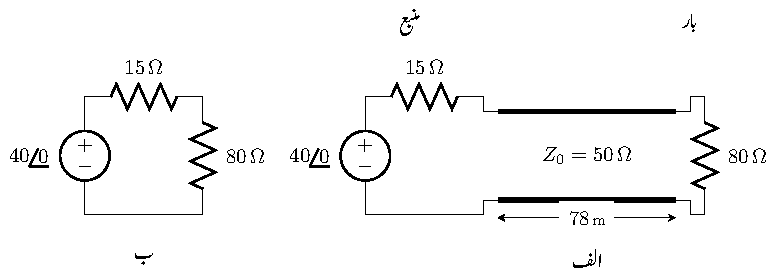
\includegraphics[width=\textwidth]{figTransmissionLineExample}
\caption{ترسیلی تار اور برقی بوجھ۔}
\label{شکل_ترسیلی_تار_بار_بردار}
\end{figure}

حل:الف) ترسیلی تار میں \عددی{\SI{500}{\kilo\hertz}} تعدد پر  طول موج اور \عددی{\beta} مندرجہ ذیل ہیں۔
\begin{align*}
\lambda&=\frac{v}{f}=\frac{2\times 10^8}{500000}=\SI{400}{\meter}\\
\beta&=\frac{2\pi}{\lambda}=\frac{2\pi}{400}=\frac{\pi}{200} \, \si{\radian\per\meter}
\end{align*}
اس تعدد پر ترسیلی تار کی لمبائی، طول موج  کے \عددی{\SI{19.5}{\percent}} ہے۔ترسیلی تار  کی داخلی قدرتی رکاوٹ
\begin{align*}
Z_{\text{داخلی}} &= 50 \frac{80+j 50 \tan (\frac{\pi}{200} \times 78)}{50+j 80 \tan (\frac{\pi}{200} \times 78)}\\
&=33.599-j 10.441
\end{align*}
ہے۔ترسیلی تار کے داخلی سرے پر \عددی{\SI{80}{\ohm}} کا برقی بوجھ \عددی{Z_{\text{داخلی}}} نظر آتا ہے۔یوں ترسیلی تار کے داخلی سرے پر برقی دباو
\begin{align*}
V_{\text{داخلی}}=\frac{40 \times (33.599-j 10.441)}{15+33.599-j 10.441}=28.2-j 2.54
\end{align*}
ہو گا۔برقی بوجھ کو \عددی{z=0} پر تصور کرنے سے  ترسیلی تار  کا داخلی سرا \عددی{z=\SI{-78}{\meter}} پر ہو گا۔ ترسیلی تار کے داخلی برقی دباو کو ترسیلی تار میں موجود آمدی موج \عددی{V^+=V_0^+ e^{-j\beta z}} اور انعکاسی موج \عددی{V^-=V_0^- e^{j \beta z}} کا نقطہ \عددی{z=\SI{-78}{\meter}} پر مجموعہ
\begin{align*}
V_{\text{داخلی}} = V_0^+ e^{-j \frac{\pi}{200} (-78)}+V_0^- e^{j \frac{\pi}{200} (78)} = V_0^+ e^{j 1.22522}+V_0^- e^{-j 1.22522}
\end{align*}
 تصور کیا جا سکتا ہے جس میں
\begin{align*}
V_0^-=\Gamma V_0^+=\left(\frac{80-50}{80+50} \right) V_0^+=\frac{3}{13} V_0^+
\end{align*}
پر کرنے سے
\begin{align*}
28.2-j 2.54 = V_0^+ e^{j 1.22522}+\frac{3}{13} V_0^+ e^{-j 1.22522}
\end{align*}
یا
\begin{align*}
V_0^+=\frac{28.2-j 2.54}{e^{j 1.22522}+\frac{3}{13} e^{-j 1.22522}}=33.9 e^{-j 1.138}
\end{align*}
حاصل ہوتا ہے۔یوں برقی بوجھ پر برقی دباو
\begin{align*}
V_L=V_0^+(1+\Gamma) = 33.9 e^{-j 1.138} \left(1+\frac{3}{13}\right)=41.7 e^{-j 1.138}=41.7 \phase{-65.2^{\circ}}
\end{align*}
ہو گا۔

آئیں برقی بوجھ کو منتقل طاقت بھی حاصل کریں۔ برقی بوجھ پر برقی دباو  کے استعمال سے اوسط طاقت
\begin{align*}
P_L=\frac{1}{2} \frac{\abs{V_L}^2}{R_L}=\frac{1}{2} \frac{41.7^2}{80}=\SI{10.88}{\watt}
\end{align*}
حاصل ہوتی ہے۔

ترسیلی تار کے داخلی سرے پر برقی رو
\begin{align*}
I_{\text{داخلی}}  = \frac{V_{\text{داخلی}}}{Z_{\text{داخلی}}} = \frac{28.2-j 2.54}{33.599-j 10.441}=0.787+j0.169
\end{align*}
ہو گی۔ یوں ترسیلی تار کو داخلی سرے پر
\begin{align*}
P_{\text{داخلی}}=\frac{1}{2} \left . V_{\text{داخلی}} I^*_{\text{داخلی}} \right|_{\text{حقیقی}}=\frac{1}{2}(28.2-j 2.54)(0.787-j0.169)=\SI{10.88}{\watt}
\end{align*}
طاقت منتقل ہو رہی ہے۔ترسیلی تار بے ضیاع ہے لہٰذا یہی طاقت برقی بوجھ کو منتقل ہو گی۔ 

ب) ترسیلی تار میں \عددی{\SI{50}{\hertz}} تعدد پر طول موج اور \عددی{\beta} مندرجہ ذیل ہیں۔
\begin{align*}
\lambda&=\frac{v}{f}=\frac{2\times 10^8}{50}=\SI{4e6}{\meter}\\
\beta&=\frac{2\pi}{\lambda}=\frac{2\pi}{4\times 10^6}=5\pi \times 10^{-7} \, \si{\radian\per\meter}
\end{align*}
اس تعدد پر ترسیلی تار کی لمبائی، طول موج سے نہایت کم \عددی{\lambda\gg\SI{78}{\meter}} ہے۔ترسیلی تار  کی داخلی قدرتی رکاوٹ
\begin{align*}
Z_{\text{داخلی}} &= Z_0 \frac{Z_L+j Z_0 \tan \beta l}{Z_0+j Z_L \tan \beta l}=50 \frac{80+j 50 \tan (5 \pi \times 10^{-7} \times 78)}{50+j 80 \tan (5 \pi \times 10^{-7} \times 78)}\\
&=50 \frac{80+j0.0061}{50+j 0.0098}=79.999998697 \phase{-0.00684^{\circ}}\\
& \approx \SI{80}{\ohm}
\end{align*}
ہے۔آپ دیکھ سکتے ہیں کہ \عددی{\beta l \ll 1} کی صورت میں \عددی{\tan \beta l \to 0} ہوتا ہے جس سے ترسیلی تار کی داخلی قدرتی رکاوٹ تقریباً برقی بوجھ کے برابر ہی حاصل ہوتی ہے۔آپ نے  دیکھا کہ \عددی{l \ll \lambda} کی صورت میں ترسیلی تار کے داخلی سرے پر برقی بوجھ جوں کا توں نظر آتا ہے لہٰذا ترسیلی تار کا ہونا یا نہ ہونا یک برابر ہے۔ایسی صورت میں ترسیلی تار کی موجودگی رد کرتے ہوئے دور کو کرخوف کے قوانین سے حل کیا جاتا ہے۔ایسا کرنے سے ہمیں شکل \حوالہ{شکل_ترسیلی_تار_بار_بردار}-ب حاصل ہوتی ہے جسے کرخوف کے قوانین کی مدد سے حل کرتے  ہوئے برقی بوجھ پر
\begin{align*}
V_L=\frac{40 \times 80}{15+80}=\SI{33.7}{\volt}
\end{align*}
برقی دباو حاصل ہوتی ہے۔
\انتہا{مثال}

مندرجہ بالا مثال میں آپ نے دیکھا کہ کسی بھی برقی دور میں  تار کی لمبائی \عددی{l} طول موج \عددی{\lambda} سے بہت کم \عددی{l \ll \lambda} ہونے کی صورت میں، ترسیلی تار کو رد کرتے ہوئے، دور کو کرخوف کے قوانین سے حل کیا جاتا ہے۔البتہ جب بھی تار کی لمبائی، طول موج کے ساتھ مطابقت رکھے، ایسی صورت میں کرخوف کے قوانین غیر کار آمد ہوتے ہیں اور میکس ویل کی مساوات سے ہی درست جوابات حاصل ہوتے ہیں۔

پاکستان میں \عددی{\SI{50}{\hertz}} اور \عددی{\SI{220}{\volt}} کی برقی طاقت مہیا کی جاتی ہے۔تار پر موج کی رفتار \عددی{\SI{3e8}{\meter\per\second}} لیتے ہوئے \عددی{\lambda=\SI{6000}{\kilo\meter}} حاصل ہوتی ہے۔گھر کے اندر فاصلے \عددی{\lambda} سے بہت کم ہوتے ہیں\حاشیہد{مجھے اپنا گھر بہت چھوٹا لگنے لگا ہے۔} لہٰذا گھر میں \عددی{\SI{484}{\ohm}} بلب کی برقی رو دریافت کرتے ہوئے  تار کی لمبائی رد کرتے ہوئے  \عددی{\tfrac{220}{484}=\SI{0.45}{\ampere}} حاصل ہوتی ہے۔اس کے برعکس تربیلا ڈیم سے کراچی شہر کا فاصلہ تقریباً \عددی{\SI{1500}{\kilo\meter}} ہے جو \عددی{\lambda} سے مناسبت رکھتا ہے، لہٰذا تربیلا ڈیم سے کراچی شہر کو برقی طاقت کے منتقلی کے مسائل حل کرتے ہوئے میکس ویل کی مساوات استعمال کرنا لازم ہو گا۔ 
%=========================
\ابتدا{مثال}
قدرتی رکاوٹ \عددی{\SI{50}{\ohm}} کے ترسیلی تار کے اختتام پر \عددی{Z_1=50-j100 \, \si{\ohm}} جڑا ہے جبکہ اختتام سے \عددی{0.2\lambda} فاصلے پر \عددی{Z_2=\SI{100}{\ohm}}  جڑا ہے۔ترسیلی تار کے دونوں حصوں میں شرح ساکن موج \عددی{s} حاصل کریں۔

حل:محدود لمبائی کی ترسیلی تار میں متعدد انعکاسی امواج پائی جاتی ہیں۔تمام آگے جانب حرکت امواج کو ایک عدد آمدی بڑھتی موج تصور کرتے ہوئے اور اسی طرح تمام واپسی جانب حرکت کرتے ہوئے تمام امواج کو ایک عدد انعکاسی موج تصور کرتے ہوئے حل کرتے ہیں۔

ترسیلی تار کے اختتامی حصے پر
\begin{align*}
\Gamma=\frac{50-j100-50}{50-j100+50}=0.5-j0.5 
\end{align*}
ہو گا جس سے  \عددی{\abs{\Gamma}=\tfrac{1}{\sqrt{2}}} حاصل ہوتا ہے۔اس قیمت کو استعمال کرتے ہوئے
\begin{align*}
s=\frac{1+\abs{\Gamma}}{1-\abs{\Gamma}}=\frac{1+\frac{1}{\sqrt{2}}}{1+\frac{1}{\sqrt{2}}}=5.83
\end{align*}
حاصل ہوتا ہے۔

جس نقطے پر \عددی{\SI{100}{\ohm}} مزاحمت جڑی ہے اس مقام پر \عددی{50-j100} سے اختتام پذیر \عددی{0.2\lambda} لمبی تار کی داخلی رکاوٹ
\begin{align*}
Z_{\text{داخلی}} &= 
50 \frac{(50-j100) +j 50 \tan \left( \frac{2\pi}{\lambda} \times 0.2 \lambda\right)}{50+j (50-j100)  \tan\left(  \frac{2\pi}{\lambda} \times 0.2 \lambda\right)}\\
&=8.63+j3.82
\end{align*}
ہے۔ اب \عددی{Z_{\text{داخلی}}} اور \عددی{\SI{100}{\ohm}} متوازی جڑے ہیں جن کا مجموعہ
\begin{align*}
\frac{100\times(8.63+j3.82)}{100+8.63+j3.82}=8.06+j3.23
\end{align*}
ہو گا۔داخلی جانب سے دیکھتے ہوئے ترسیلی تار کو \عددی{\SI{100}{\ohm}} کی بجائے \عددی{8.06+j3.23} برقی بوجھ نظر آئے گا۔یوں ترسیلی تار کے داخلی حصے پر
\begin{align*}
\Gamma=\frac{8.06+j3.23-50}{8.06+j3.23+50}=-0.717+j0.096=0.723 \phase{171.9^{\circ}}
\end{align*} 
اور
\begin{align*}
s=\frac{1+0.723}{1-0.723}=6.22
\end{align*}
ہوں گے۔
\انتہا{مثال}
%============================
\حصہ{ترسیمی تجزیہ، سمتھ نقشہ}
\اصطلاح{سمتھ نقشہ}\فرہنگ{سمتھ نقشہ}\حاشیہب{Smith chart}\فرہنگ{Smith chart} بنیادی طور پر شرح انعکاس
\begin{align*}
\Gamma=\frac{Z_L-Z_0}{Z_L+Z_0}
\end{align*}
کی مساوات پر منحصر ہے۔اس نقشے میں برقی بوجھ بمطابق \عددیء{Z_0} یعنی  \عددیء{\tfrac{Z_L}{Z_0}} استعمال کی جاتی ہے جسے
\begin{align*}
z=r+jx=\frac{Z_L}{Z_0}=\frac{R_L+j X_L}{Z_0}
\end{align*}
لکھا جا سکتا ہے جہاں \عددیء{z} کارتیسی محدد کا متغیرہ نہیں بلکہ \عددیء{Z_0} کے مطابقت سے برقی بوجھ کو ظاہر کرتا ہے۔یوں
\begin{align*}
\Gamma=\frac{z-1}{z+1}
\end{align*}
  اور
\begin{align}\label{مساوات_ترسیلی_انعکاس_بالمقابل_قدرتی_رکاوٹ}
z=\frac{1+\Gamma}{1-\Gamma}
\end{align}
لکھے جا سکتے ہیں۔شرح انعکاس کو حقیقی اور خیالی اجزاء
\begin{align*}
\Gamma=\Gamma_r+j \Gamma_i
\end{align*}
کی صورت میں لکھتے ہوئے
\begin{align*}
r+j x =\frac{1+\Gamma_r+j \Gamma_i}{1-\Gamma_r-j\Gamma_i}
\end{align*} 
کے حقیقی اور خیالی اجزاء علیحدہ کرتے ہوئے
\begin{align}
r&=\frac{1-\Gamma_r^2-\Gamma_i^2}{\left(1-\Gamma_r\right)^2+\Gamma_i^2}\\
x&=\frac{2\Gamma_i}{\left(1-\Gamma_r\right)^2+\Gamma_i^2}
\end{align}
لکھے جا سکتے ہیں جنہیں کچھ الجبرا کے بعد
\begin{align}
\left(\Gamma_r-\frac{r}{1+r}\right)^2+\Gamma_i^2&=\left(\frac{1}{1+r}\right)^2 \label{مساوات_ترسیلی_سمتھ_دائرہ_الف}\\
\left(\Gamma_r-1 \right)^2+\left(\Gamma_i-\frac{1}{x} \right)^2&=\left(\frac{1}{x}\right)^2  \label{مساوات_ترسیلی_سمتھ_دائرہ_ب}
\end{align}
لکھا جا سکتا ہے۔اگر کارتیسی محدد کے متغیرات \عددیء{\Gamma_r} اور \عددیء{\Gamma_i} رکھے جائیں تو مندرجہ بالا دونوں مساوات گول دائروں کی مساوات ہوں گی۔

مساوات \حوالہ{مساوات_ترسیلی_سمتھ_دائرہ_الف} کے دائروں پر پہلے غور کرتے ہیں۔اگر \عددیء{r=0} ہو تب یہ مساوات اکائی رداس کا دائرہ دیتی ہے جس کا وسط محدد کے  مبدا \عددیء{(0,0)} پر ہے۔خیالی برقی بوجھ کی صورت میں شرح انعکاس کی مطلق قیمت ایک ہی ہوتی ہے۔اسی طرح \عددیء{r=\infty} کی صورت میں دائرے کا رداس صفر جبکہ اس کا وسط  \عددیء{(1,0)} پر ہے۔یوں یہ دائرہ صرف اسی نقطے یعنی \عددیء{\Gamma=1} تک محدود ہے۔اب \عددیء{r=\infty} سے مراد \عددیء{Z_L-\infty} ہے جس سے شرح انعکاس \عددیء{\Gamma=1} ہی حاصل ہوتی ہے۔ایک آخری مثال \عددیء{r=1} کی لیتے ہیں جس سے \عددیء{0.5} رداس کا دائرہ حاصل ہوتا ہے جس کا وسط \عددیء{(0.5,0)} ہے۔شکل \حوالہ{شکل_ترسیلی_سمتھ-نقشہ_الف} میں ان دائروں کے علاوہ \عددیء{r=0.5} اور \عددیء{r=2} سے حاصل دائرے بھی  دکھایا گیا ہے۔ 

\begin{figure}
\centering
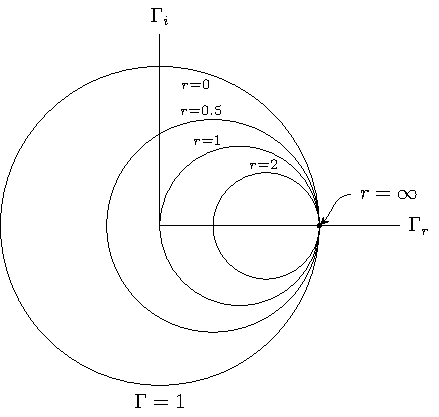
\includegraphics{figTransmissionSmithRealPart}
\caption{کارتیسی محدد کے متغیرات \عددیء{\Gamma_r} اور \عددیء{\Gamma_i} ہیں جبکہ دائرے کا رداس \عددیء{\tfrac{1}{r+1}} ہے۔}
\label{شکل_ترسیلی_سمتھ-نقشہ_الف}
\end{figure}

مساوات \حوالہ{مساوات_ترسیلی_سمتھ_دائرہ_ب} بھی دائرے دیتی ہے البتہ ان دائروں کا رداس \عددیء{\tfrac{1}{x}} اور مراکز \عددیء{(1,\tfrac{1}{x})} ہیں۔لامحدود \عددیء{x} کی صورت میں دوبارہ \عددیء{Z=\infty} اور \عددیء{{\Gamma=1+j0}} ہوں گے۔مساوات \حوالہ{مساوات_ترسیلی_سمتھ_دائرہ_ب} کے مطابق اس دائرے کا رداس صفر جبکہ اس کا وسط \عددیء{(1,0)} ہے لہٰذا یہ \عددیء{\Gamma=1} کو ہی ظاہر کرتا ہے۔اگر \عددیء{x=1} ہو تب دائرے کا رداس اکائی جبکہ اس کا وسط \عددیء{(1,1)} ہوں گے۔جیسا شکل \حوالہ{شکل_ترسیلی_سمتھ-نقشہ_ب} میں دکھایا گیا ہے، اس دائرے کا چوتھائی حصہ \عددیء{\abs{\Gamma}=1} دائرے کے اندر پایا جاتا ہے۔اسی طرح \عددیء{x=-1} کی صورت میں دائرے کا چوتھائی حصہ  \عددیء{\Gamma_r} محدد کے نیچے پایا جاتا ہے۔شکل میں \عددیء{x=0.5}، \عددیء{x=-0.5}، \عددیء{x=2} اور \عددیء{x=-2} کے دائرے بھی دکھائے گئے ہیں۔شکل میں \عددیء{x=0} سے پیدا سیدھی لکیر، یعنی \عددیء{\Gamma_r} محدد بھی دکھایا گیا ہے۔
\begin{figure}
\centering
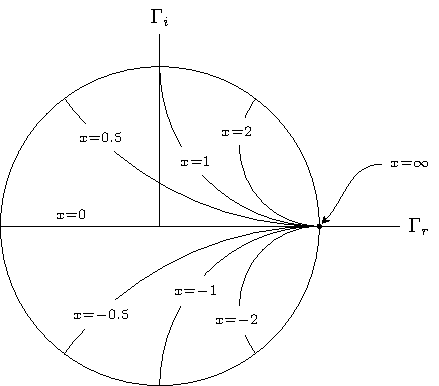
\includegraphics{figTransmissionSmithImaginaryPart}
\caption{کارتیسی محدد پر $\tfrac{1}{x}$ رداس کے دائروں کے وہ حصے دکھائے گئے ہیں جو اکائی دائرے کے اندر پائے جاتے ہیں۔}
\label{شکل_ترسیلی_سمتھ-نقشہ_ب}
\end{figure}

ان دونوں دائروں کو ایک ہی جگہ شکل \حوالہ{شکل_ترسیلی_سمتھ-نقشہ_پ} کے سمتھ نقشے میں دکھایا گیا ہے۔یوں کسی بھی \عددیء{Z_L} کی صورت میں \عددیء{\tfrac{Z_L}{Z_0}} کی شرح لیتے ہوئے \عددیء{z} یعنی \عددیء{r} اور \عددیء{x} حاصل کر کے  سمتھ نقشے میں ان کے دائروں کی نشاندہی کریں۔اگر نقشے پر درکار \عددیء{r} اور (یا) \عددیء{x} کے دائرے نہ پائے جائیں تب ان کے قریبی قیمتوں کے دائروں سے مطلوبہ دائرے کا مقام اخذ کریں۔جہاں یہ دائرے  ایک دوسرے کو کاٹتے ہیں وہاں سے  \عددیء{\Gamma} پڑھیں۔نقشے  کے مبدا \عددیء{(0,0)} سے  اس نقطے تک فاصلہ \عددیء{\abs{\Gamma}} کے برابر ہو گا جبکہ افقی محدد یعنی \عددیء{\Gamma_r} سے گھڑی کے الٹ سمت زاویہ \عددیء{\Gamma} کا زاویہ ہو گا۔اس زاویے کو اکائی رداس کے دائرے کے باہر دکھایا گیا ہے۔یوں محدد کے مبدا سے درکار نقطے تک سیدھی لکیر کو اکائی رداس کے دائرے تک بڑھا کر زاویہ ناپا جاتا ہے۔ سمتھ نقشے میں \عددیء{\abs{\Gamma}} ناپنے کی غرض سے محدد کے مبدا \عددیء{(0,0)} پر مختلف رداس کے دائرے کھینچے جا سکتے تھے، لیکن ایسا نہیں کیا جاتا۔آپ کو یہ فاصلہ نقشے میں دئے فیتے کی مدد سے ناپنا ہو گا۔اب مثال کے طور پر \عددیء{Z_0=\SI{50}{\ohm}} کی ترسیلی تار پر \عددیء{Z_L=25+j50 \,\si{\ohm}} کا برقی بوجھ \عددیء{z=0.5+j1} سے ظاہر کیا جائے گا۔اس نقطے کو شکل میں بطور نقطہ \عددیء{N} دکھایا گیا ہے جو \عددیء{r=0.5} اور \عددیء{x=1} کے دائروں کے نقطہ ملاپ سے حاصل ہوتا ہے۔شرح انعکاس تقریباً \عددیء{0.62\phase{83^\circ}}  حاصل ہوتا ہے۔
\begin{figure}
\centering
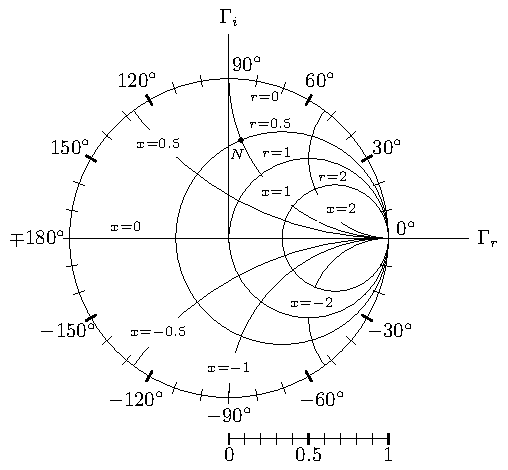
\includegraphics{figTransmissionSmithChart}
\caption{سمتھ نقشے پر اکائی دائرے میں $r$ اور $x$ سے حاصل دائرے دکھائے جاتے ہیں۔}
\label{شکل_ترسیلی_سمتھ-نقشہ_پ}
\end{figure}

سمتھ نقشہ مکمل کرنے کی خاطر اکائی دائرے کے  محیط کے باہر دوسرا فیتہ شامل کیا جاتا ہے جس سے ترسیلی تار پر فاصلہ ناپا جاتا ہے۔اس فیتے پر فاصلہ طول موج \عددیء{\lambda} کی صورت میں ناپا جا سکتا ہے۔آئیں دیکھیں کہ اس فیتے سے کس طرح فاصلہ حاصل کیا جاتا ہے۔ترسیلی تار پر کسی بھی نقطے پر برقی دباو
\begin{align*}
V_s=V_0^+ \left(e^{-j\beta z}+\Gamma e^{j \beta z} \right)
\end{align*}
کو برقی رو
\begin{align*}
I_s =\frac{V_0^+}{Z_0}\left(e^{-j\beta z}-\Gamma e^{j \beta z} \right)
\end{align*}
سے تقسیم کرتے ہوئے \عددیء{Z_0} کے مطابقت سے داخلی قدرتی رکاوٹ
\begin{align*}
z_{\text{داخلی}} = \frac{Z_{\text{داخلی}}}{Z_0}=\frac{V_s}{Z_0 I_s}=\frac{e^{-j\beta z}+\Gamma e^{j \beta z} }{e^{-j\beta z}-\Gamma e^{j \beta z} }
\end{align*}
حاصل کی جا سکتی ہے جس میں \عددیء{z=-l} پر کرتے ہوئے
\begin{align}\label{مساوات_ترسیلی_داخلی_رکاوٹ_سمتھ_الف}
z_{\text{داخلی}} =\frac{1+\Gamma e^{-j 2\beta l}}{1-\Gamma e^{j 2\beta l}}
\end{align}
لکھا جا سکتا ہے۔اس مساوات میں \عددیء{l=0} پر کرنے سے
\begin{align}\label{مساوات_ترسیلی_داخلی_رکاوٹ_سمتھ_ب}
\left. z_{\text{داخلی}} \right|_{l=0}=\frac{1-\Gamma}{1+\Gamma} = z
\end{align}
حاصل ہوتا ہے جو عین برقی بوجھ پر شرح انعکاس ہے جسے مساوات \حوالہ{مساوات_ترسیلی_انعکاس_بالمقابل_قدرتی_رکاوٹ} میں پیش کیا گیا ہے۔

یہاں رک کر اس حقیقت پر غور کریں کہ \عددیء{\Gamma} کو \عددیء{e^{-j2\beta l}} سے ضرب دینے سے
\begin{align*}
\Gamma e^{-j2 \beta l}= \abs{\Gamma} e^{j \phi} e^{-j 2 \beta l}= \abs{\Gamma} e^{j(\phi-2\beta l)}
\end{align*}
حاصل ہوتا ہے جس کی مطلق قیمت اب بھی \عددیء{\abs{\Gamma}} ہی ہے  لیکن نیا زاویہ \عددیء{(\phi-2\beta l)} ہے۔یوں سمتھ نقشے میں نقطہ \عددیء{z} یعنی 
\begin{align}\label{مساوات_ترسیلی_داخلی_رکاوٹ_سمتھ_پ}
z=r+j x=\frac{1+\Gamma}{1-\Gamma}
\end{align}
کی نشاندہی کرتے ہوئے  \عددیء{\abs{\Gamma} \phase{\phi}} ناپیں۔اب \عددیء{\abs{\Gamma}} تبدیل کئے بغیر زاویہ تبدیل کرتے ہوئے \عددیء{(\phi-2\beta l)} تک پہنچیں اور یہاں سے \عددیء{z_{\text{داخلی}}}  ناپیں۔آپ دیکھ سکتے ہیں کہ مساوات \حوالہ{مساوات_ترسیلی_داخلی_رکاوٹ_سمتھ_پ} میں \عددیء{\Gamma} کی جگہ \عددیء{\Gamma e^{-j 2\beta l}} پر کرنے سے مساوات \حوالہ{مساوات_ترسیلی_داخلی_رکاوٹ_سمتھ_الف} ہی حاصل ہوتا ہے جو برقی بوجھ سے \عددیء{l} فاصلے پر بمطابق \عددیء{Z_0} داخلی قدرتی رکاوٹ ہے۔

یوں برقی بوجھ \عددیء{z} سے دور \عددیء{z_{\text{داخلی}}} کی طرف چلتے ہوئے، ہم منبع طاقت یعنی جنریٹر کی طرف چلتے ہیں جبکہ سمتھ نقشے پر ایسا کرنے سے زاویہ \عددیء{\phi} سے کم ہو کر \عددیء{\phi-2\beta l} ہوتا ہے لہٰذا نقشے پر ہم گھڑی کی سمت چلتے ہیں۔یوں \عددیء{\beta l=\pi} فاصلہ، یعنی آدھی طول موج، طے کرنے سے نقشے کے گرد ایک چکر مکمل ہو گا۔اس طرح \عددیء{\tfrac{\lambda}{2}} لمبی  بے ضیاع ترسیلی تار کی داخلی قدرتی رکاوٹ عین برقی بوجھ کے رکاوٹ برابر ہو گی۔

یوں سمتھ نقشے کے حیطے پر ایک مکمل چکر کو \عددیء{0.5 \lambda} دکھایا جاتا ہے۔جیسے شکل \حوالہ{شکل_ترسیلی_مکمل_سمتھ_نقشہ} میں دکھایا گیا ہے، استعمال میں آسانی کی غرض سے ایک کے بجائے دو ایسے  فیتے بنائے جاتے ہیں۔ایک فیتہ گھڑی کی سمت میں بڑھتا فاصلہ دکھاتا ہے جسے نقشے میں \قول{منجانب جنریٹر} سے ظاہر کیا جاتا ہے جبکہ دوسرا فیتہ گھڑی کی الٹ سمت بڑھتا فاصلہ دکھاتا ہے جسے \قول{منجانب بار} لکھ کر ظاہر کیا جاتا ہے۔ان فیتوں کے ابتدائی نقطے کوئی اہمیت نہیں رکھتے البتہ انہیں نقشے کے بائیں ہاتھ پر رکھا جاتا ہے۔ آپ کو یاد ہو گا کہ حقیقی \عددیء{Z_L} اور \عددیء{Z_0} کی صورت میں اگر \عددیء{Z_L<Z_0} ہو تب برقی دباو کا نشیب اسی نقطے پر ہو گا۔
\begin{figure}
\centering
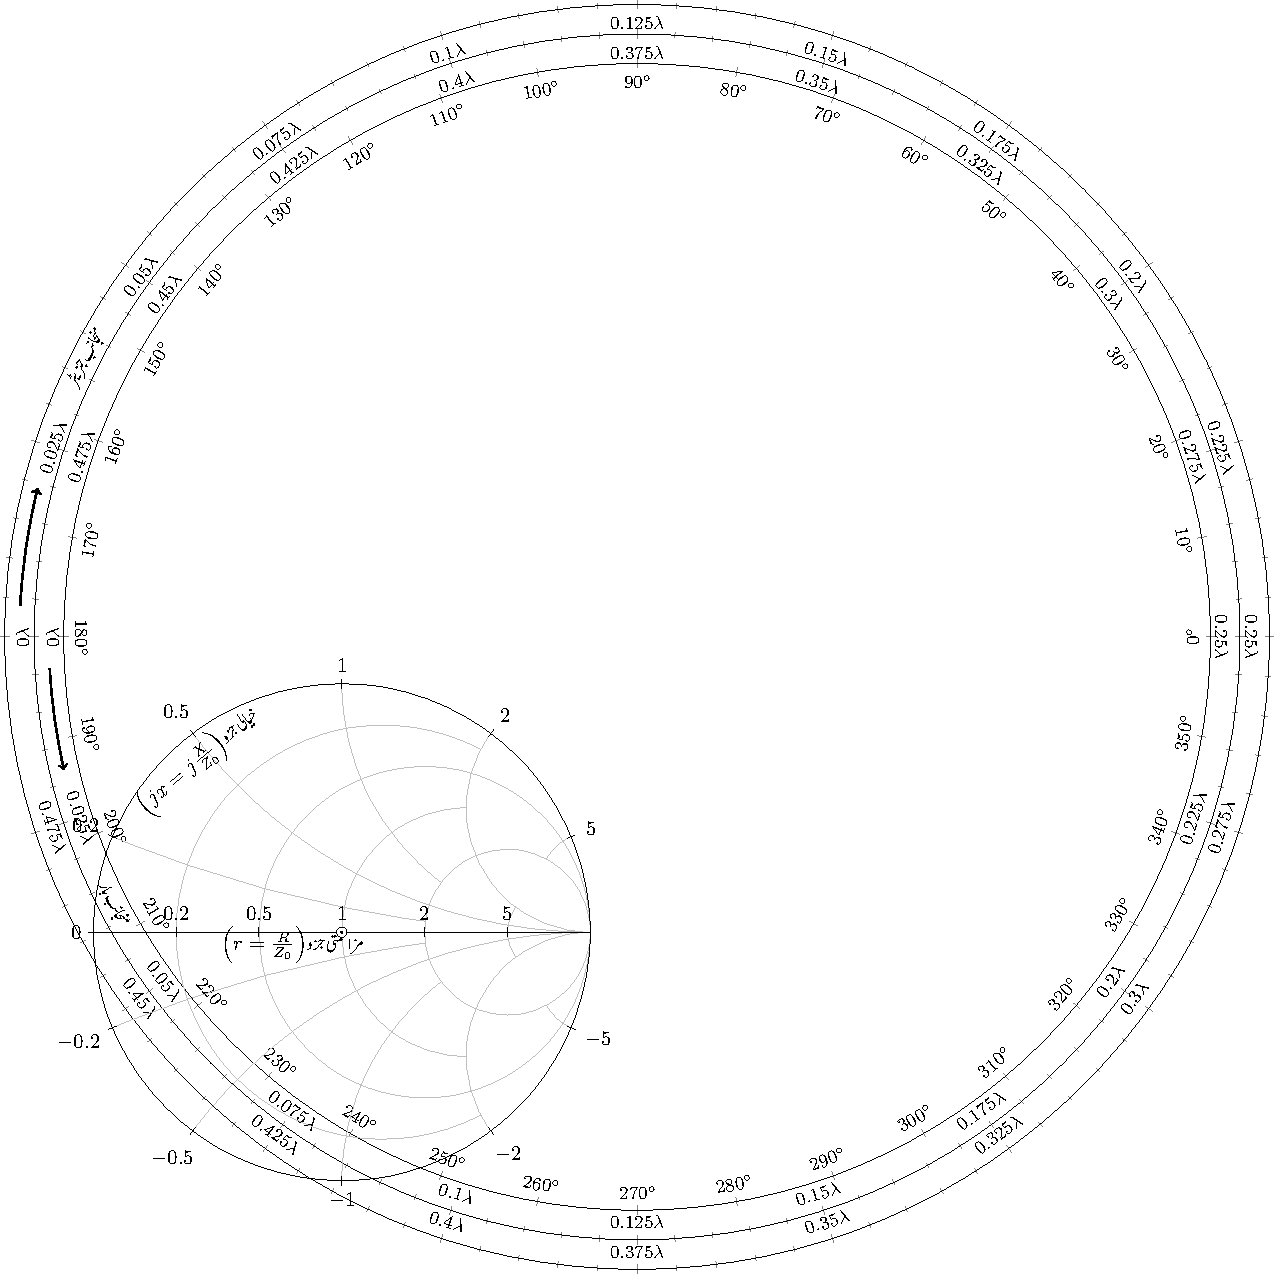
\includegraphics[width=\textwidth]{figTransmissionSmithFromInternet}
\caption{مکمل سمتھ نقشہ۔}
\label{شکل_ترسیلی_مکمل_سمتھ_نقشہ}
\end{figure} 

سمتھ نقشے کا استعمال مثال کی مدد سے بہتر سمجھا جا سکتا ہے۔یوں \عددیء{\SI{50}{\ohm}} کی ترسیلی تار پر \عددیء{Z_L=25+j 50 \, \si{\ohm}} کے برقی بوجھ پر دوبارہ غور کرتے ہیں۔شکل \حوالہ{شکل_ترسیلی_ایک_تہائی_تار} میں \عددیء{z=0.5+j 1} کو نقطہ \عددیء{A} ظاہر کرتا ہے جہاں سے \عددیء{\Gamma=0.62 e^{j 1.45}=0.62\phase{83^\circ}} حاصل ہوتا ہے۔مبدا سے \عددیء{A} تک لکیر کو اکائی دائرے کے حیطے تک بڑھا کر \عددیء{0.135 \lambda} پڑھا جاتا ہے۔اگر تار کی لمبائی \عددیء{\SI{60}{\centi\meter}} ہو اور اشارے کی تعدد اتنی ہو  کہ ترسیلی تار پر طول موج \عددیء{\SI{2}{\meter}} ہو، تب \عددیء{\tfrac{l}{\lambda}=0.3} ہو گا لہٰذا تار \عددیء{0.3 \lambda} لمبی ہو گی۔یوں  بیرونی دائرے پر \عددیء{0.135\lambda+0.3\lambda=0.435\lambda} سے مبدا تک لکیر  اور \عددیء{\abs{\Gamma}} رداس کے دائرے کے ملاپ، یعنی نقطہ \عددیء{B}، سے  \عددیء{z_{\text{داخلی}}=0.28-j0.4}  حاصل ہوتا ہے۔اس طرح \عددیء{Z_{\text{داخلی}}=14-j 20} ہو گا۔تحلیلی طور پر زیادہ درست جواب \عددیء{Z_{\text{داخلی}}=13.7-j 20.2} حاصل ہوتا ہے۔

\begin{figure}
\centering
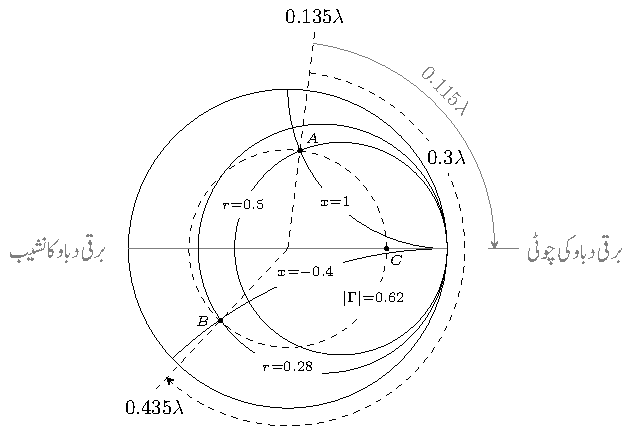
\includegraphics{figTransmissionSmithChartLambdaByThree}
\caption{سمتھ نقشے سے متغیرات کا حصول۔}
\label{شکل_ترسیلی_ایک_تہائی_تار}
\end{figure}

سمتھ نقشے سے موج کی چوٹی یا نشیب کے مقام باآسانی حاصل کئے جاتے ہیں۔کسی بھی \عددیء{\Gamma=\abs{\Gamma}\phase{\phi}} کے لئے \عددیء{z=-l} پر آمدی اور انعکاسی امواج کے مجموعے
\begin{align*}
V_s&=V_0^+ \left(e^{j\beta l} +\Gamma e^{-j \beta l}\right)\\
&=V_0^+ e^{j \beta l} \left[1+\abs{\Gamma} e^{j\left(\phi-2 \beta l\right)} \right]
\end{align*}

کی مطلق قیمت
\begin{align*}
\abs{V_s} &=V_0^+ \abs{e^{j\beta l}} \left[\abs{1+\abs{\Gamma} e^{j\left( \phi-2 \beta l\right)} }\right]\\
&=V_0^+\abs{1+\abs{\Gamma} e^{j\left(\phi-2 \beta l\right)} }
\end{align*}
ہے جہاں \عددیء{\abs{e^{j\beta l}}=1} کے برابر\حاشیہد{\عددیء{\abs{e^{j\beta l}}=\abs{\cos \beta l+j\sin\beta l}=\sqrt{\cos^2 \beta l +\sin^2 \beta l}=1}} ہے۔اس کی کم سے کم قیمت \عددیء{V_0^+ \left(1-\abs{\Gamma} \right)} ہے جو \عددیء{\phi-\beta l= (2 n +1)\pi} کی صورت میں حاصل ہوتی ہے جہاں \عددیء{n=0,1,2,\cdots} ہے۔عین برقی بوجھ پر \عددیء{l=0} ہے اور ایسی صورت میں اس شرط کو \عددیء{\phi= \pi} لکھا جا سکتا ہے۔اسی طرح \عددیء{\abs{V_s}} کی زیادہ سے زیادہ قیمت \عددیء{V_0^+ \left(1+\abs{\Gamma} \right)} ہے جو \عددیء{\phi-\beta l=2 n \pi} کی صورت میں حاصل ہوتی ہے جہاں \عددیء{n=0,1,2,\dots} ہے۔عین برقی بوجھ پر \عددیء{l=0} ہے اور ایسی صورت میں اس شرط کو
 \عددیء{\phi=0} لکھا جا سکتا ہے۔یوں \عددیء{\phi= \pi} کی صورت میں برقی بوجھ پر \عددیء{V_s} کی کم سے کم قیمت ہو گی جبکہ \عددیء{\phi=0} کی صورت میں برقی بوجھ پر \عددیء{V_s} کی زیادہ سے زیادہ قیمت ہو گی۔آئیں دیکھیں کہ ان شرائط کا مطلب کیا ہے۔


مزاحمتی برقی بوجھ \عددیء{R_L} اور حقیقی \عددیء{Z_0} کی صورت میں اگر \عددیء{R_L<Z_0} ہو تب \عددیء{\Gamma} منفی حقیقی عدد ہو گا جسے  \عددیء{\Gamma=\abs{\Gamma}\phase{\pi}} لکھا جا سکتا ہے جبکہ \عددیء{R_L>Z_0} کی صورت میں \عددیء{\Gamma} مثبت حقیقی عدد ہو گا جسے  \عددیء{\Gamma=\abs{\Gamma}\phase{0^\circ}} لکھا جا سکتا ہے۔یوں \عددیء{R_L<Z_0} یعنی \عددیء{\Gamma=\abs{\Gamma}\phase{0}} کی صورت میں برقی بوجھ پر کمتر \عددیء{V_s} ہو گا جبکہ \عددیء{R_L>Z_0} یعنی \عددیء{\Gamma=\abs{\Gamma}\phase{\pi}} کی صورت میں برقی بوجھ پر بلند تر \عددیء{V_s} ہو گا۔سمتھ نقشے پر افقی محدد حقیقی \عددیء{\Gamma} دیتا ہے۔منفی افقی محدد پر  \عددیء{\Gamma=\abs{\Gamma}\phase{\pi}} ہوتا ہے لہٰذا برقی بوجھ پر کمتر \عددیء{V_s} ہر صورت سمتھ نقشے میں منفی افقی محدد پر پایا جائے گا۔اسی طرح مثبت افقی محدد پر  \عددیء{\Gamma=\abs{\Gamma}\phase{0}} ہوتا ہے لہٰذا برقی بوجھ پر بلند تر \عددیء{V_s} ہر صورت سمتھ نقشے میں مثبت افقی محدد پر پایا جائے گا۔

ان نتائج کو آگے بڑھاتے ہیں۔کسی بھی مخلوط برقی بوجھ \عددیء{Z_L=R_L+j X_L} کی صورت میں سمتھ نقشے میں \عددیء{z=r+j x} سے شروع کر کے فاصلہ \عددیء{l} بڑھانے سے زاویہ \عددیء{\phi-2\beta l} گھٹتا ہے جو سمتھ نقشے پر گھڑی کی سمت گھومنے کے مترادف ہے۔جس فاصلے پر \عددیء{\phi-2\beta l =2n\pi} ہو وہاں برقی موج کی چوٹی پائی جائے گی اور جس فاصلے پر \عددیء{\phi-2\beta l=(2n+1)\pi} ہو وہاں موج کا نشیب پایا جائے گا۔اب \عددیء{2n\pi} سے مراد سمتھ نقشے کے افقی محدد کا مثبت حصہ جبکہ
 \عددیء{(2n+1)\pi} سے مراد افقی محدد کا منفی حصہ ہے۔ یوں شکل \حوالہ{شکل_ترسیلی_ایک_تہائی_تار} میں نقطہ \عددیء{A} سے گھڑی کی سمت \عددیء{0.115 \lambda} گھومتے ہوئے  ترسیلی تار پر پہلی چوٹی پائی جائے گی۔یوں برقی بوجھ سے پہلی چوٹی \عددیء{0.115\lambda} یعنی \عددیء{0.115 \times 200=\SI{23}{\centi\meter}} فاصلے پر ہے۔ اگر ترسیلی تار زیادہ لمبی ہوتی تب برقی بوجھ سے \عددیء{0.365\lambda} دور پہلا نشیب پایا جاتا۔چونکہ تار کی لمبائی اس سے کم ہے لہٰذا تار پر کہیں پر بھی نشیب نہیں پایا جاتا۔

برقی رو کی چوٹی اس نقطے پر پائی جاتی ہے جہاں \عددیء{\phi-2\beta l =2n \pi} کا شرط پورا ہو۔برقی رو
\begin{align*}
I_s=\frac{V_0^+}{Z_0} \left (e^{j \beta l}-\Gamma e^{j \beta l} \right)
\end{align*}
کی کمتر قیمت اس نقطے پر پائی جاتی ہے۔اسی طرح جس نقطے پر برقی دباو کی کمتر قیمت پائی جائے، اس نقطے پر برقی رو کی چوٹی پائی جاتی ہے۔یوں سمتھ نقشے کے افقی محدد کے مثبت حصے پر برقی رو کا نشیب جبکہ اس کے منفی حصے پر برقی رو کی چوٹی پائی جائے گی۔

مزاحمتی برقی بوجھ \عددیء{R_L} اور بے ضیاع ترسیلی تار کی صورت میں \عددیء{\Gamma=\tfrac{R_L-R_0}{R_L+R_0}} ہو گا۔اگر \عددیء{R_L>R_0} ہو تب 
\عددیء{\abs{\Gamma}=\frac{R_L-R_0}{R_L+R_0}} ہو گا جبکہ \عددیء{R_L<R_0}  کی صورت میں \عددیء{\abs{\Gamma}=\frac{R_0-R_L}{R_0+R_L}} ہو گا۔یوں \عددیء{R_L>R_0} کی صورت میں
\begin{align*}
s=\frac{1+\abs{\Gamma}}{1-\abs{\Gamma}}=\frac{1+\frac{R_L-R_0}{R_L+R_0}}{1-\frac{R_L-R_0}{R_L+R_0}}=\frac{R_L}{R_0}=r \quad{(R_L>R_0)}
\end{align*}
جبکہ \عددیء{R_L<R_0} کی صورت میں
\begin{align*}
s=\frac{1+\abs{\Gamma}}{1-\abs{\Gamma}}=\frac{1+\frac{R_0-R_L}{R_0+R_L}}{1-\frac{R_0-R_L}{R_0+R_L}}=\frac{R_0}{R_L} \quad{(R_L<R_0)}
\end{align*}
ہو گا۔یاد رہے کہ \عددیء{s>1} ہوتا ہے لہٰذا \عددیء{\tfrac{R_L}{R_0}} اور \عددیء{\tfrac{R_0}{R_L}} میں جو بھی اکائی سے زیادہ قیمت رکھتا ہو یہی \عددیء{s} ہو گا۔یوں \عددیء{\abs{\Gamma}} رداس کے دائرے اور مثبت افقی محدد سے \عددیء{r} پڑھ کر \عددیء{s} کی قیمت بھی یہی تصور کریں۔شکل \حوالہ{شکل_ترسیلی_ایک_تہائی_تار} میں نقطہ \عددیء{C} سے \عددیء{r=4.2} پڑھا جائے گا لہٰذا \عددیء{s=4.2} ہے۔مثبت افقی محدد پر \عددیء{r>1} ہوتا ہے لہٰذا محدد کے اسی حصے سے \عددیء{s} کی قیمت پڑھی جاتی ہے۔ آپ تسلی کر لیں کہ \عددیء{\tfrac{R_0}{R_L}>1} کی صورت میں بھی اسی طریقہ کار سے درست \عددیء{s} حاصل ہوتا ہے۔

%=============================
\جزوحصہ{سمتھ فراوانی نقشہ}
اس حصے کو \عددیء{\tfrac{\lambda}{4}} لمبی تار کی داخلی قدرتی رکاوٹ کے حصول سے شروع کرتے ہیں۔اتنی لمبائی کے تار کا \عددیء{\beta l =90^\circ} ہو گا۔ داخلی قدرتی رکاوٹ کی مساوات
\begin{align*}
Z_{\text{داخلی}}=Z_{0} \frac{Z_{L}+j Z_{0}\tan \beta l}{Z_{0}+j Z_{L}\tan \beta l}
\end{align*}
میں \عددیء{Z_{\text{داخلی}}} کو \عددیء{Z_0} سے تقسیم کرتے اور  \عددیء{\beta l =90^\circ} پر کرتے ہوئے
\begin{align*}
\frac{Z_{\text{داخلی}}}{Z_{0}}= \frac{Z_{L}+j Z_{0}\tan 90^\circ}{Z_{0}+j Z_{L}\tan 90^\circ}=\frac{Z_0}{Z_L}
\end{align*}

یعنی
\begin{align}\label{مساوات_ترسیلی_فراوانی_اور_رکاوٹ_الف}
 z_{\!\!\! {\scriptstyle{\overset{\text{داخلی}}{0.25\lambda}}}}\!\!\! =\frac{1}{z}
\end{align}
حاصل ہوتا ہے جہاں
\begin{align*}
\frac{Z_{\text{داخلی}}}{Z_{0}}& =  z_{\!\!\! {\scriptstyle{\overset{\text{داخلی}}{0.25\lambda}}}} \\
\frac{Z_L}{Z_0}&=z
\end{align*}
لکھے گئے ہیں۔مساوات \حوالہ{مساوات_ترسیلی_فراوانی_اور_رکاوٹ_الف} کے تحت برقی بوجھ سے \عددیء{0.25\lambda} فاصلے پر  داخلی قدرتی رکاوٹ \عددیء{\tfrac{1}{z}} کے برابر ہے  لیکن \عددیء{\tfrac{1}{z}=y} ہوتا ہے لہٰذا اسی مساوات کو یوں بھی لکھا جا سکتا ہے
\begin{align}\label{مساوات_ترسیلی_فراوانی_اور_رکاوٹ_ب}
y=\frac{1}{z}= z_{{\scriptstyle \overset{\text{\RL{منجانب جنریٹر}}}{0.25\lambda}}}
\end{align}
جہاں \عددیء{0.25\lambda} تار کی داخلی قدرتی رکاوٹ کی جگہ منجانب جنریٹر  \عددیء{0.25\lambda} گھومنے کا ذکر کیا گیا ہے۔مساوات \حوالہ{مساوات_ترسیلی_فراوانی_اور_رکاوٹ_ب} کہتی ہے کہ سمتھ نقشے میں \عددیء{z} سے منجانب جنریٹر \عددیء{0.25\lambda} گھوم کر \عددیء{\abs{\Gamma}} رداس کے دائرے سے \عددیء{y} حاصل ہو گا۔

\begin{figure}
\centering
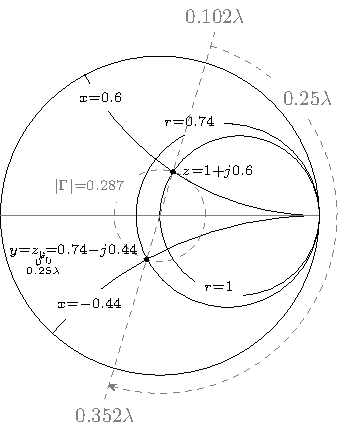
\includegraphics{figTransmissionSmithAdmittanceAsQuarterLineImpedance}
\caption{چوتھائی طول تار کی داخلی قدرتی رکاوٹ اسی تار کی برقی فراوانی کے برابر ہے۔}
\label{شکل_ترسیلی_سمتھ_فراوانی_اور_چوتھائی_طول}
\end{figure}

شکل \حوالہ{شکل_ترسیلی_سمتھ_فراوانی_اور_چوتھائی_طول} میں \عددیء{z=1+j 0.6} دکھایا گیا ہے جو منجانب جنریٹر \عددیء{0.102 \lambda} زاویے پر پایا جاتا ہے۔یہ رکاوٹ \عددیء{\Gamma=0.287 \phase{73.7^\circ}} دیتا ہے۔چوتھائی طول لمبی تار کی داخلی قدرتی رکاوٹ حاصل کرنے کی خاطر منجانب جنریٹر \عددیء{0.25\lambda} چلتے ہوئے \عددیء{0.352\lambda} سے مبدا تک لکیر اور \عددیء{0.287} رداس کے دائرے کے ملاپ سے  \عددیء{z_{\text{داخلی}}=0.74-j0.44} حاصل ہوتا ہے جو \عددیء{\tfrac{1}{z}} یعنی \عددیء{y} کے عین برابر ہے۔

آئیں قصر دور اور کھلے دور تار کے ٹکڑوں کا داخلی قدرتی رکاوٹ حاصل کریں۔قصر دور تار کی صورت میں \عددیء{Z_L=0} ہو گا لہٰذا داخلی قدرتی رکاوٹ
\begin{gather}
\begin{aligned}\label{مساوات_ترسیلی_قصر_دور_ٹکڑا_بطور_امالہ}
Z_{\text{داخلی}}&=Z_{0} \frac{0+j Z_{0}\tan \beta l}{Z_{0}+j 0\tan \beta l}\\
&=j Z_0 \tan \beta l
\end{aligned}
\end{gather}
حاصل ہوتا ہے جو خیالی عدد ہے۔چوتھائی طول لمبی قصر دور تار کی داخلی قدرتی رکاوٹ یوں
\begin{align}
Z_{\scriptstyle \overset{\text{داخلی}}{0.25\lambda}}=j Z_0 \tan 90^\circ= \infty \quad \quad(\text{\RL{قصر دور}})
\end{align}
حاصل ہوتی ہے۔یہ تعجب بھرا نتیجہ ہے جس کے مطابق چوتھائی طول لمبی کسے دور تار بطور کھلے دور کردار ادا کرتی ہے۔

کھلے  دور تار کی صورت میں \عددیء{Z_L=\infty} ہو گا لہٰذا داخلی قدرتی رکاوٹ
\begin{gather}
\begin{aligned}\label{مساوات_ترسیلی_کھلے_دور_ٹکڑا_بطور_کپیسٹر}
Z_{\text{داخلی}}&=Z_{0} \frac{\infty+j Z_{0}\tan \beta l}{Z_{0}+j \infty\tan \beta l}\\
&=-j \frac{Z_0}{ \tan \beta l }
\end{aligned}
\end{gather}
حاصل ہوتا ہے جو خیالی عدد ہے۔چوتھائی طول لمبی کھلے دور تار کی داخلی قدرتی رکاوٹ یوں
\begin{align}
Z_{\scriptstyle \overset{\text{داخلی}}{0.25\lambda}}=-j \frac{Z_0}{ \tan 90^\circ}= 0 \quad \quad(\text{\RL{کھلے دور}})
\end{align}
حاصل ہوتی ہے۔یہ بھی تعجب بھرا نتیجہ ہے جس کے مطابق چوتھائی طول لمبی کھلے دور تار بطور قصر دور کردار ادا کرتی ہے۔

سمتھ مزاحمتی نقشے\فرہنگ{سمتھ!مزاحمتی نقشہ}\فرہنگ{Smith!impedance chart}\حاشیہب{Smith impedance chart} کا متبادل سمتھ فراوانی\فرہنگ{سمتھ!فراوانی نقشہ}\فرہنگ{Smith!admittance chart}\حاشیہب{Smith admittance chart} نقشہ بھی استعمال کیا جاتا ہے۔ ان میں \عددیء{y=\tfrac{Y_L}{Y_0}=g+jb} لیا جاتا ہے جہاں \عددیء{Y_L=\tfrac{1}{R_L}} اور \عددیء{Y_0=\tfrac{1}{Z_0}} کے برابر ہیں۔اس طرح \عددیء{y} برقی فراوانی بمطابق \عددیء{Y_0} کہلائے گی۔یوں \عددیء{r} سے حاصل دائرے اب \عددیء{g} کے دائرے کہلاتے ہیں جبکہ \عددیء{x} کے دائرے \عددیء{b} کے دائرے کہلاتے ہیں۔اس نقشے میں \عددیء{g>1} اور \عددیء{b=0} کی صورت میں برقی دباو کی کمتر قیمت حاصل ہو گی۔ ایصالی سمتھ نقشے سے حاصل \عددیء{\Gamma} کا زاویہ \عددیء{180^\circ} بڑھانا ہو گا۔

%======================
\حصہ{تجرباتی نتائج پر مبنی چند مثال}
اس حصے میں دو مثالوں پر غور کیا جائے گا۔پہلی مثال میں تجرباتی نتائج سے برقی بوجھ کی رکاوٹ حاصل کی جائے گی جبکہ دوسری مثال میں برقی بوجھ کو تار کے ہمہ رکاوٹ بنانے کی ترکیب دکھائی جائے گی۔

ہم محوری ترسیلی تار کے بیرونی تار میں لمبائی کی سمت میں شگاف ڈال کر اس میں مختلف مقامات پر برقی دباو کے نمونے لے کر \عددیء{s=2.5} حاصل کیا گیا ہے۔شکل \حوالہ{شکل_ترسیلی_ہم_محوری_شگاف_دار} میں ایسی \اصطلاح{شگاف دار تار}\فرہنگ{شگاف دار تار}\حاشیہب{slotted line}\فرہنگ{slotted line} دکھائی گئی ہے۔شگاف کے ساتھ فیتہ رکھ کر بلند تر اور کم تر نمونوں کے مقامات بھی درج کئے گئے۔ایسے نتائج حاصل کرتے وقت فیتے کا صفر کہیں پر بھی رکھا جا سکتا ہے لہٰذا اسے برقی بوجھ کا مقام تصور نہیں کریں۔کمتر برقی دباو فیتے پر \عددیء{\SI{47}{\centi\meter}} کے نشان کے ساتھ پایا جاتا ہے۔سائن نما اشارے کی صورت میں سمت کار کے خارجی اشارہ شکل میں دکھایا گیا ہے۔آپ دیکھ سکتے ہیں کہ اشارے کے کمتر قیمت کا مقام ٹھیک ٹھیک تعین کرنا زیادہ آسان ہے۔اشارے کی چوٹی نوک دار نہیں ہوتی لہٰذا اس کا مقام ٹھیک ٹھیک تعین کرنا قدر مشکل ہوتا ہے۔اسی وجہ سے عموماً موج کی کمتر قیمت کے مقامات حاصل کرتے ہوئے مطلوبہ معلومات دریافت کی جاتی ہیں۔ہم محوری تار کی قدرتی رکاوٹ \عددیء{\SI{50}{\ohm}} ہے اور تار  میں ہوا بطور ذو برق استعمال کی گئی ہے۔اشارے کی تعدد \عددیء{\SI{400}{\mega\hertz}} ہے لہٰذا طول موج \عددیء{\SI{75}{\centi\meter}} ہے۔برقی بوجھ کا مقام تعین کرنے کی خاطر برقی بوجھ کو ہٹا کر تار کے ان سروں کو قصر دور کیا جاتا ہے۔قصر دور تار پر کمتر دباو فیتے پر \عددیء{\SI{26}{\centi\meter}} کے نشان کے سامنے پایا جاتا ہے۔

\begin{figure}
\centering
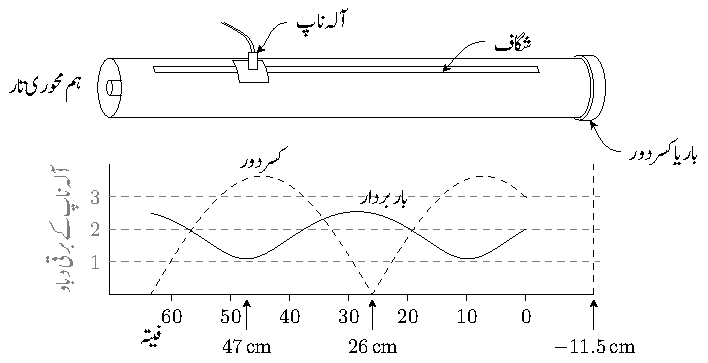
\includegraphics{figTransmissionSlottedLine}
\caption{ہم محوری تار میں شگاف ڈال کر اس میں آلہ ناپ کی مدد سے مختلف مقامات پر برقی دباو  کے نمونے لئے جا سکتے ہیں۔}
\label{شکل_ترسیلی_ہم_محوری_شگاف_دار}
\end{figure}
ہم جانتے ہیں کہ قصر دور نقطے سے کمتر دباو کا فاصلہ \عددیء{\tfrac{n\lambda}{2}} ہو گا۔ہم فرض کرتے ہیں کہ کمتر دباو قصر دور نقطے سے آدھے طول موج کے فاصلے پر ہے۔ایسی صورت میں قصر دور کا مقام فیتے پر \عددیء{26-37.5=\SI{-11.5}{\centi\meter}} نشان کے ساتھ ہو گا۔چونکہ برقی بوجھ کے مقام پر ہی قصر دور پیدا کیا گیا تھا لہٰذا برقی بوجھ بھی فیتے پر \عددیء{\SI{-11.5}{\centi\meter}} کے نشان کے ساتھ ہو گا۔یوں حاصل نتائج کے تحت برقی بوجھ سے کم تر دباو کا نقطہ \عددیء{47-(-11.5)=\SI{58.5}{\centi\meter}} فاصلے پر ہے جس سے آدھی طول موج منفی کرتے ہوئے برقی بوجھ سے کمتر دباو کا فاصلہ \عددیء{\SI{21}{\centi\meter}} حاصل ہوتا ہے۔بلند تر دباو کا برقی بوجھ سے فاصلہ یوں
 \عددیء{21-\tfrac{37.5}{2}=\SI{2.25}{\centi\meter}} ہو گا جو \عددیء{\tfrac{2.25}{75}=0.03} طول موج کے برابر ہے۔
\begin{figure}
\centering
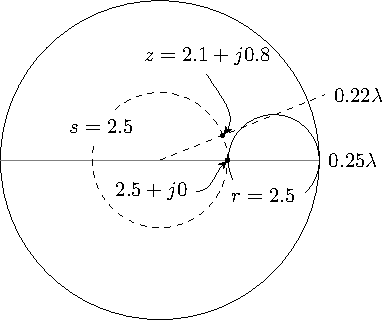
\includegraphics{figTransmissionSmithChartSlottedLine}
\caption{اگر $0.03\lambda$ لمبی تار پر $z_{\text{داخلی}}=2.5+j0$ ہو تب $z=2.1+j0.8$ ہو گا۔}
\label{شکل_ترسیلی_ہم_محوری_تجرباتی_نتائج}
\end{figure}

ان معلومات کے ساتھ اب شکل \حوالہ{شکل_ترسیلی_ہم_محوری_تجرباتی_نتائج} کے سمتھ نقشے کا سہارا لیتے ہیں۔بلند تر برقی دباو کے نقطے پر  داخلی قدرتی رکاوٹ حقیقی عدد ہوتا ہے جس کی قیمت \عددیء{s R_0} کے برابر ہوتی ہے، لہٰذا ایسے نقطے پر \عددیء{z_{\text{داخلی}}=2.5} ہو گا۔ہم یوں سمتھ نقشے پر \عددیء{z_{\text{داخلی}}=2.5} نقطے پر داخل ہوتے ہیں جہاں سے منجانب جنریٹر فاصلہ \عددیء{0.25\lambda} پڑھا جاتا ہے۔اس سے \عددیء{0.03\lambda} منفی کرتے ہوئے  برقی بوجھ تک پہنچتے ہیں، لہٰذا \عددیء{0.22\lambda} سے مبدا تک لکیر اور \عددیء{s=2.5} یعنی     \عددیء{\abs{\Gamma}=0.429} رداس کے دائرے کے ملاپ سے \عددیء{z=2.1+j0.8} پڑھا جاتا ہے۔یوں \عددیء{Z_L=105+j40 \, \si{\ohm}} حاصل ہوتا ہے۔یاد رہے کہ ہم نے برقی بوجھ کو فیتے پر \عددیء{\SI{-11.5}{\centi\meter}} یا اس نقطے سے \عددیء{\tfrac{n\lambda}{2}} فاصلے پر تصور کیا ہے۔چونکہ برقی بوجھ کا مقام اب بھی مکمل طور پر معلوم نہیں ہے لہٰذا بہتر یہ ہوتا ہے کہ تجرباتی نتائج سے حاصل \عددیء{Z_L} کی بات کرتے ہوئے برقی بوجھ کا فرض کردہ مقام بھی ساتھ بتلایا جائے۔

آخر میں آئیں اس برقی بوجھ کو \عددیء{\SI{50}{\ohm}} ترسیلی تار کے ہمہ رکاوٹ بنانے کی ترکیب دیکھیں۔ایسا \عددیء{d_1} لمبائی کے قصر دور تار کے ٹکڑے کو برقی بوجھ سے \عددیء{d} فاصلے پر نسب کرنے سے ممکن بنایا جاتا ہے۔ایسا شکل \حوالہ{شکل_ترسیلی_ہمہ_رکاوٹی_بمدد_ٹکڑا_تار} میں دکھایا گیا ہے۔برقی بوجھ سے \عددیء{d} فاصلے پر \عددیء{z_{داخلی}} کے متوازی \عددیء{d_1} لمبی قصر دور ٹکڑا نسب کرنے سے کل رکاوٹ \عددیء{z=1+j0} حاصل کرنے مقصد ہے۔یہاں \عددیء{d_1} اور \عددیء{d} مطلوب ہیں۔قصر دور ٹکڑے کی قدرتی رکاوٹ ترسیلی تار کی قدرتی رکاوٹ \عددیء{\SI{50}{\ohm}} کے برابر ہے۔ 

\begin{figure}
\centering
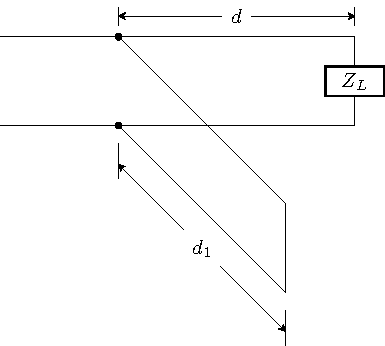
\includegraphics{figTransmissionLoadParallelStud}
\caption{برقی بوجھ سے $d$ فاصلے پر $d_1$ لمبائی کے قصر دور تار کا ٹکڑا جوڑنے سے برقی بوجھ اور اور ترسیلی تار ہمہ رکاوٹ بنائے جاتے ہیں۔}
\label{شکل_ترسیلی_ہمہ_رکاوٹی_بمدد_ٹکڑا_تار}
\end{figure}

برقی بوجھ اور قصر دور تار کا ٹکڑا متوازی جڑے ہیں۔متوازی جڑی رکاوٹوں کی بجائے متوازی جڑی برقی فراوانی کے ساتھ کام کرنا زیادہ آسان ہوتا ہے لہٰذا ہم ایسا ہی کرتے ہیں۔برقی فراوانی کی زبان میں موجودہ مسئلہ کچھ یوں ہے۔ہم \عددیء{d} اتنا رکھنا چاہتے ہیں کہ داخلی فراوانی \عددیء{y_{\text{داخلی}}=1+jb} ہو۔اب اگر \عددیء{y_{\text{داخلی}}} کے متوازی \عددیء{-j b} برقی تاثریت جوڑی جائے تو حاصل کل برقی فراوانی \عددیء{1+j0} ہو گی جو ہمارا مقصد ہے۔یوں \عددیء{d_1} لمبی قصر دور تار کے ٹکڑے کی برقی تاثریت \عددیء{-jb} درکار ہے۔ان حقائق کو لے کر سمتھ نقشے کی مدد سے \عددیء{d} اور \عددیء{d_1} کی قیمتیں حاصل کرتے ہیں۔

\begin{figure}
\centering
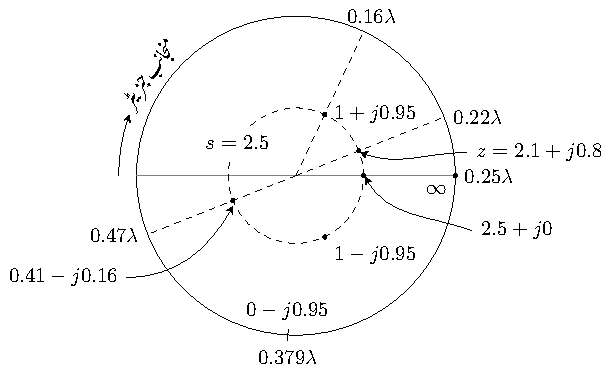
\includegraphics{figTransmissionSmithChartMatchingStud}
\caption{برقی بوجھ $z=2.1+j0.8$ سے $0.19\lambda$ فاصلے پر $0.129\lambda$ لمبائی کا قصر دور ٹکڑا جوڑنے سے نظام ہمہ رکاوٹ ہو جاتا ہے۔}
\label{شکل_ترسیلی_ہمہ_رکاوٹی_ٹکڑے_کا_نقشہ}
\end{figure}

سمتھ نقشے میں \عددیء{z=2.1+j0.8} پر داخلی ہو کر مساوات \حوالہ{مساوات_ترسیلی_فراوانی_اور_رکاوٹ_ب} کے تحت منجانب جنریٹر \عددیء{0.25\lambda} گھومنے سے \عددیء{y=\tfrac{1}{z}} حاصل ہوتا ہے۔شکل \حوالہ{شکل_ترسیلی_ہمہ_رکاوٹی_ٹکڑے_کا_نقشہ} میں ایسا دکھایا گیا ہے۔سمتھ نقشے میں \عددیء{z=2.1+j0.8} منجانب جنریٹر \عددیء{0.22\lambda} زاویے پر پایا جاتا ہے۔یہاں سے منجانب جنریٹر \عددیء{0.25\lambda} گھومتے ہوئے \عددیء{0.47\lambda} تک پہنچا جاتا ہے جہاں \عددیء{\abs{\Gamma}} رداس کے دائرے سے \عددیء{y=0.41-j0.16} ملتا ہے۔اب ہم چاہتے ہیں کہ یہاں سے  منجانب جنریٹر  گھومتے ہوئے  داخلی قدرتی فراوانی \عددیء{1+jb} حاصل ہو۔جیسا شکل میں دکھایا گیا ہے، ایسا \عددیء{0.16\lambda} اور \عددیء{0.34\lambda} زاویوں پر ممکن ہے جہاں سے بالترتیب \عددیء{y_1=1+j0.95} اور  \عددیء{y_2=1-j0.95} حاصل ہوتے ہیں۔پہلے نقطے تک پہنچنے کے لئے کم لمبائی کی تار درکار ہے لہٰذا اسی کو جواب تسلیم کرتے ہیں۔برقی بوجھ سے اس نقطے تک \عددیء{(0.5\lambda-0.47\lambda)+0.16\lambda=0.19\lambda} تار درکار ہو گی لہٰذا \عددیء{d=0.19\lambda} یعنی \عددیء{\SI{14.25}{\centi\meter}} بنتا ہے۔

 اب \عددیء{1+j 0.95} کے متوازی \عددیء{y_{\text{ٹکڑا}}=-j0.95} برقی تاثریت جوڑ کر \عددیء{1+j0} حاصل ہو گا۔مساوات \حوالہ{مساوات_ترسیلی_کھلے_دور_ٹکڑا_بطور_کپیسٹر} کے تحت قصر دور ٹکڑے کی داخلی رکاوٹ یا داخلی فراوانی خیالی عدد ہوتا ہے لہٰذا سمتھ نقشے پر ایسے ٹکڑے کا \عددیء{g=0} ہی رہے گا جو نقشے کی بیرونی دائرے کو ظاہر کرتی ہے۔عین قصر دور پر \عددیء{y=\infty} حاصل ہوتا ہے جو منجانب جنریٹر  \عددیء{0.25\lambda} پر پایا جاتا ہے۔ہم دیکھتے ہیں کہ \عددیء{y_{\text{داخلی}}=-j0.95} نقشے پر منجانب جنریٹر \عددیء{0.379\lambda} پر حاصل ہوتا ہے۔یوں کسے دور ٹکڑے کی لمبائی \عددیء{0.379\lambda-0.25\lambda=0.129\lambda} یعنی \عددیء{\SI{9.67}{\centi\meter}} حاصل ہوتا ہے۔   

%===================
\ابتدا{مشق}
بے ضیاع \عددیء{\SI{50}{\ohm}} ترسیلی تار کو قصر دور کرنے سے برقی دباو کے دو آپس میں قریبی نشیب \عددیء{\SI{12}{\centi\meter}} اور \عددیء{\SI{27}{\centi\meter}} پر پائے جاتے ہیں۔ قصر دور ختم کرتے ہوئے یہاں برقی بوجھ نسب کرنے سے \عددیء{\SI{0.4}{\volt}} حیطے کے نشیب اور \عددیء{\SI{0.72}{\volt}} حیطے کی چوٹیاں حاصل ہوتی ہیں۔ ایک عدد نشیب \عددیء{\SI{9}{\centi\meter}} پر حاصل ہوتا ہے۔ترسیلی تار میں ہوا بطور ذو برق استعمال ہوئی ہے۔مندرجہ ذیل حاصل کریں۔ \عددیء{\lambda}، \عددیء{f}، \عددیء{s}، \عددیء{\Gamma} اور \عددیء{Z_L}

جوابات:\عددیء{\SI{0.3}{\meter}}، \عددیء{\SI{1}{\giga\hertz}}، \عددیء{1.8}،
 \عددیء{0.286\phase{108^\circ}} اور \عددیء{36.5+j21.6\, \si{\ohm}}
\انتہا{مشق}
%===================
\ابتدا{مشق}
بے ضیاع \عددیء{\SI{50}{\ohm}} کے ساتھ \عددیء{Z_L=100+j100 \, \si{\ohm}} کا برقی بوجھ نسب ہے۔برقی بوجھ سے \عددیء{d} فاصلے پر \عددیء{d_1} لمبائی کا قصر دور ٹکڑا جوڑتے ہوئے نظام کو ہمہ رکاوٹ بنایا جاتا ہے۔اگر تار پر \عددیء{v=\tfrac{2}{3}c} ہو جبکہ اشارے کی تعدد \عددیء{\SI{10}{\mega\hertz}} ہو تب مندرجہ ذیل حاصل کریں۔ \عددیء{\lambda}، چھوٹے سے چھوٹا \عددیء{d_1} اور ایسی صورت میں \عددیء{d}

جوابات:\عددیء{\SI{20}{\meter}}، \عددیء{\SI{1.8}{\meter}} اور \عددیء{\SI{4.4}{\meter}}
\انتہا{مشق}
%=================
\حصہ{پیما شرح ساکن موج}
شرح ساکن موج ناپنے کے لئے شگاف دار تار استعمال کرنا شکل \حوالہ{شکل_ترسیلی_ہم_محوری_شگاف_دار} میں دکھایا گیا۔شرح ساکن موج ناپنے کے لئے مخصوص آلہ شکل \حوالہ{شکل_ترسیلی_آلہ_پیما_شرح_ساکن_موج} میں دکھایا گیا ہے جسے ہم \اصطلاح{پیما شرح ساکن موج}\فرہنگ{پیما!شرح ساکن موج}\فرہنگ{ساکن موج!پیما شرح}\حاشیہب{directional coupler}\فرہنگ{directional coupler} کہیں گے۔اس شکل میں \عددی{x} محدد پر پڑی، ہم محوری تار کے اندر دو عدد اضافی موصل تار رکھے گئے ہیں۔بالائی اضافی تار کے دائیں سرے کو مزاحمت \عددی{R_1} کے ذریعہ بیرونی تار کے ساتھ جوڑا گیا ہے جبکہ اس کا بایاں سرا بیرونی تار میں سوراخ سے باہر نکالا گیا ہے۔اس اضافی تار کی لمبائی \عددی{l} جبکہ اس کی قدرتی رکاوٹ \عددی{R_1} ہے۔نچلی اضافی تار کے بائیں سرے کو مزاحمت \عددی{R_1} کے ذریعہ بیرونی تار کے ساتھ جوڑا گیا ہے جبکہ اس کا دایاں سرا بیرونی تار میں سوراخ سے باہر نکالا گیا ہے۔اس اضافی تار کی لمبائی بھی \عددی{l} اور اس کی قدرتی رکاوٹ \عددی{R_1} ہے۔

\begin{figure}
\centering
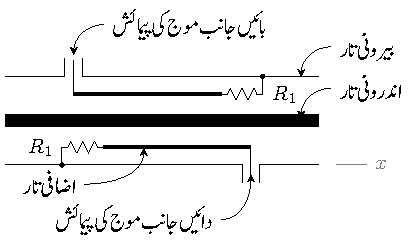
\includegraphics{figTransmissionDirectionalCoupler}
\caption{پیما شرح ساکن موج}
\label{شکل_ترسیلی_آلہ_پیما_شرح_ساکن_موج}
\end{figure}

پیما کو منبع طاقت اور برقی بوجھ کے درمیان ترسیلی تاروں کے ذریعہ نسب کیا جاتا ہے۔تصور کریں کہ منبع طاقت بائیں جانب جڑی  ہے جبکہ برقی بوجھ دائیں جانب جڑا ہے۔یوں ہم محوری تار میں منبع سے برقی بوجھ کی جانب آمدی موج حرکت کرے گی جبکہ برقی بوجھ سے منبع کی جانب انعکاسی موج حرکت کرے گی۔آمدی موج دونوں اضافی تاروں میں بھی برقی بوجھ کی جانب حرکت کرتی موج پیدا کرے گی۔بالائی تار میں یہ موج مزاحمت \عددی{R_1} پر اختتام پذیر ہو گی۔چونکہ اضافی تار کی قدرتی رکاوٹ بھی \عددی{R_1} ہے لہٰذا تار کے دائیں سرے پر انعکاس نہیں ہو پائے گا۔نچلی اضافی تار میں دائیں جانب حرکت کرتا میدان  برقی دباو \عددی{v_i=E_{xi} l} پیدا کرے گا جو تار کے باہر نکالے گئے سرے پر پایا جائے گا۔یوں آمدی موج صرف نچلی تار میں برقی دباو پیدا کرتی ہے۔اسی طرح انعکاسی موج بھی دونوں اضافی تاروں میں حرکت کرتی موج پیدا کرتی ہے۔نچلی اضافی تار میں ایسی موج \عددی{R_1} پر اختتام پذیر ہوتی ہے جبکہ بالائی اضافی تار میں یہ \عددی{v_r=E_{xr} l} برقی دباو پیدا کرتی ہے جسے تار کے باہر نکالے گئے سرے پر ناپا جا سکتا ہے۔اگر اضافی تاروں کی لمبائی اور موٹائی بالکل برابر ہو اور انہیں ہم محوری تار کے اندر بالکل یکساں جگہوں پر رکھا جائے تب دونوں اضافی تاروں میں پیدا برقی دباو آمدی اور انعکاسی امواج کے مماثل ہو گی۔یوں شرح انعکاس کو
\begin{align}
\abs{\Gamma}=\frac{v_r}{v_i}
\end{align}
اور شرح ساکن موج کو
\begin{align}
s=\frac{1+\abs{\Gamma}}{1-\abs{\Gamma}}
\end{align}
سے ناپا جا سکتا ہے۔

پیما کے استعمال سے  تبدیلی مزاحمت کے شرح ساکن موج پر اثرات کو دیکھا جاتا ہے۔اسی طرح ایسی منبع طاقت جو تعددی پٹی پر طاقت پیدا کر سکتی ہو کے استعمال سے تعدد بالمقابل \عددی{s} دیکھا جاتا ہے۔
%================================
\حصہ{تجزیہ عارضی حال}\شناخت{حصہ_ترسیلی_عارضی_حال}
اب تک ہم  ترسیلی تار میں کسی ایک تعدد پر، \اصطلاح{برقرار یکساں حال}\فرہنگ{برقرار یکساں حال}\حاشیہب{steady state}\فرہنگ{steady state} سائن نما امواج کی بات کرتے رہے ہیں۔اس حصے میں غیر سائن نما امواج کی بات کرتے ہیں۔آپ جانتے ہیں کہ کسی بھی غیر سائن نما موج کو فوریئر تسلسل کی مدد سے متعدد اجزاء کا مجموعہ لکھا جا سکتا ہے جہاں ہر جزو کی تعدد مختلف ہوتی ہے۔کسی بھی ترسیلی تار کے مستقل \عددی{R}، \عددی{L}، \عددی{G} اور \عددی{C} ازخود تعدد پر منحصر ہوتے ہیں۔اس کی مثال، ہم محوری تار کی مزاحمت ہے جو موٹائی جلد پر منحصر ہے جہاں موٹائی جلد کا دارومدار از خود تعدد پر ہے۔ ترسیلی تار میں موج کی رفتار ان مستقل پر منحصر ہے لہٰذا مختلف تعدد کی امواج تار میں مختلف رفتار سے حرکت کریں گی۔یوں غیر سائن نما موج کے فوریئر اجزاء مختلف رفتار سے حرکت کریں گے جس سے موج کی صورت برقرار نہیں رہ پائے گی۔حرکت کے دوران موج کی صورت بگڑنے کو \اصطلاح{انتشار}\فرہنگ{انتشار}\حاشیہب{dispersion}\فرہنگ{dispersion} کہا جاتا ہے۔فوریئر تسلسل کے انفرادی رفتار \عددی{v_p} کو \اصطلاح{دوری رفتار}\فرہنگ{دوری رفتار}\فرہنگ{رفتار!دوری}\حاشیہب{phase velocity}\فرہنگ{phase velocity} کہا جاتا ہے جبکہ منتشر ہوتے موج کی رفتار \عددی{v_g} کو \اصطلاح{مجموعی رفتار}\فرہنگ{مجموعی رفتار}\فرہنگ{رفتار!مجموعی}\حاشیہب{group velocity}\فرہنگ{group velocity} کہا جاتا ہے۔ اس کتاب میں اثر انتشار سے آزاد امواج پر غور کیا جائے گا۔ یوں دوری رفتار اور مجموعی رفتار برابر ہوں گے۔اس رفتار کو \عددی{v} لکھتے ہوئے ہم دیکھتے ہیں کہ وقت \عددی{t} میں ایسی موج \عددی{v t}  فاصلہ طے کرے گی۔

غیر سائن نما امواج میں مستطیل موج نہایت اہمیت کی حامل ہے۔\اصطلاح{عددی}\فرہنگ{عددی اشارہ}\حاشیہب{digital}\فرہنگ{digital} اشارات یعنی صفر اور  ایک  کو عددی ادوار  میں \عددی{\SI{0}{\volt}} اور \عددی{\SI{5}{\volt}} سے ظاہر کیا جاتا ہے۔عددی صفر سے عددی ایک یا عددی ایک سے عددی صفر کو سیڑھی نما تفاعل ظاہر کرتی ہے جبکہ صفر سے ایک اور واپس صفر کو مستطیل تفاعل ظاہر کرتی ہے۔یہ مستطیل یا سیڑھی نما اشارات، ترسیلی تاروں کے ذریعہ ایک جگہ سے دوسری جگہ منتقل ہوتے ہیں۔ یہ اشارات عموماً بلا ترتیب ہوتے ہیں۔آئیں ایسی ہی ایک عدد سیڑھی نما اشارے کی ترسیل پر غور کریں۔ اس طرز کے تجزیے کو \اصطلاح{عارضی رد عمل}\فرہنگ{عارضی رد عمل}\حاشیہب{transient response}\فرہنگ{transient response} کہا جاتا ہے۔

 شکل \حوالہ{شکل_ترسیلی_ابتدائی_موج} میں \عددی{Z_0} قدرتی رکاوٹ کا ترسیلی تار \عددی{Z_0} برقی بوجھ کو طاقت فراہم کرنے کے لئے استعمال کیا جا رہا ہے۔منبع طاقت کی اندرونی رکاوٹ صفر کے برابر ہے۔لمحہ \عددی{t=0} پر سوئچ کو چالو حالت میں کرتے ہوئے منبع کو ترسیلی تار کے ساتھ جوڑا جاتا ہے جس سے ترسیلی تار کا داخلی سرا \عددی{V_0} برقی دباو پر پہنچ جاتا ہے۔ترسیلی تار کا بقایا حصہ اور برقی بوجھ فی الحال \عددی{\SI{0}{\volt}} پر ہی رہتے ہیں۔سوئچ کو چالو حالت میں ہی رکھا جاتا ہے۔ تار کے داخلی سرے پر لاگو برقی دباو رفتار \عددی{v} سے اختتامی جانب حرکت کرے گی۔یوں لمحہ \عددی{t} پر یہ موج \عددی{v t} فاصلہ طے کر چکی ہو گی لہٰذا منبع سے فاصلہ \عددی{vt} تک ترسیلی تار پر اب برقی دباو \عددی{V_0} ہو گا جبکہ بقایا تار اب بھی صفر برقی دباو پر ہو گی۔شکل \حوالہ{شکل_ترسیلی_ابتدائی_موج} میں لمحہ \عددی{t} پر منبع کے ساتھ ترسیلی تار کی \عددی{vt} لمبائی حصے کو موٹی لکیر سے دکھایا گیا ہے جبکہ بقایا تار کو پتلی لکیر سے ظاہر کیا گیا ہے۔نقطہ دار لکیر اس مقام کو ظاہر کر رہی ہے جہاں برقی دباو کی موج \عددی{V^+}  پہنچ پائی ہے۔موج کے حیطے کی قیمت  \عددی{V^+=V_0} ہو گی۔تار پر برقی دباو کی صورت \اصطلاح{سیڑھی نما تفاعل}\فرہنگ{سیڑھی نما تفاعل}\حاشیہب{step function}\فرہنگ{step function} ہے۔ترسیلی تار کی لمبائی \عددی{l} ہونے کی صورت میں برقی دباو کی موج،  برقی بوجھ تک \عددی{\tfrac{l}{v}} دورانیے میں پہنچے گی جہاں \عددی{v} موج کی مجموعی رفتار ہے۔اس دورانیے میں \اصطلاح{عارضی صورت حال}\فرہنگ{عارضی صورت حال}\حاشیہب{transient state}\فرہنگ{transient state} پائی جاتی ہے۔چونکہ برقی بوجھ کی قیمت عین ترسیلی تار کے قدرتی رکاوٹ کے  برابر ہے لہٰذا \عددی{\Gamma=\tfrac{Z_L-Z_0}{Z_L+Z_0}=0} ہو گا۔یوں تار کے اختتامی سرے پر انعکاسی موج پیدا نہیں ہو گی۔اس طرح سوئچ چالو حالت میں کرنے کے ٹھیک \عددی{\tfrac{l}{v}}  دیر بعد برقی بوجھ پر منبع کی برقی دباو \عددی{V_0} پائی جائے گی۔برقی بوجھ پر اس کے بعد برقی دباو برقرار \عددی{V_0} قیمت پر رہتا ہے۔

برقی دباو کی موج کے ساتھ ساتھ برقی رو کی موج بھی پائی جاتی ہے۔یوں لمحہ \عددی{t=0} پر سوئچ چالو حالت میں کرتے ہی ترسیلی تار کے داخلی سرے پر \عددی{I^+} برقی رو کی موج پیدا ہو گی جہاں \عددی{I^+=\tfrac{V^+}{Z_0}} کے برابر ہے۔اگرچہ موصل تار میں برقی رو، منفی بار کی حرکت سے پیدا ہوتی ہے، \اصطلاح{روایتی برقی رو}\فرہنگ{روایتی برقی رو}\فرہنگ{برقی رو!روایتی}\حاشیہب{conventional current}\فرہنگ{current!conventional} کو مثبت بار کی حرکت سے ظاہر کیا جاتا ہے۔ شکل \حوالہ{شکل_ترسیلی_ابتدائی_موج} میں روایتی برقی رو ہی دکھائی گئی ہے۔یوں مثبت تار میں برقی رو کی سمت منبع سے برقی بوجھ کی جانب ہے جبکہ منفی تار میں اس کی سمت برقی بوجھ سے منبع کی جانب ہے۔دھیان رہے کہ برقی رو صرف اور صرف نقطہ دار لکیر کے اس طرف پائی جاتی ہے جس طرف منبع نسب ہے۔یوں اس شکل میں مثبت تار میں منبع سے لے کر نقطہ دار لکیر تک مثبت برقی رو پائی جائے گی جبکہ نقطہ دار لکیر کے دوسری جانب برقی رو صفر کے برابر ہو گی۔تار کے اس حصے کو موٹی لکیر سے دکھایا گیا ہے جس میں برقی رو پائی جاتی ہے۔سوئچ چالو کرنے کے ٹھیک \عددی{\tfrac{l}{v}} دیر بعد برقی بوجھ میں برقرار \عددی{\tfrac{V_0}{Z_0}} برقی رو  پائی جائے گی۔

شکل \حوالہ{شکل_ترسیلی_ابتدائی_موج} میں نقطہ دار لکیر کے دائیں جانب برقی دباو صفر کے برابر ہے۔اس جانب ترسیلی تار کو برق گیر (کپیسٹر)  تصور کرتے ہوئے آپ دیکھ سکتے ہیں کہ تار کا یہ حصہ بے بار  ہے۔اس کے برعکس نقطہ دار لکیر کے بائیں جانب برقی دباو \عددی{V_0} ہے۔یوں تار کا یہ حصہ بار بردار ہے۔مثبت تار پر برقی رو، مثبت بار کو نقطہ دار لکیر کے دائیں جانب منتقل کر رہی ہے۔اسی طرح منفی تار پر برقی رو، نقطہ دار لکیر کے دائیں جانب حصے سے مثبت بار نکال رہی ہے۔اس طرح نقطہ دار لکیر کے قریب دائیں جانب تار بار بردار ہو رہا ہے جس کی وجہ سے اس حصے کی برقی دباو بڑھتی ہے۔یہی برقی موج ہے۔

آپ دیکھ سکتے ہیں کہ  سوئچ چالو کرنے سے \عددی{\tfrac{l}{v}} تک کے عارضی دورانیے کے دوران \اصطلاح{کرخوف}\فرہنگ{کرخوف}\حاشیہب{Kirchoff's laws} کے قوانین کار آمد نہیں ہیں۔عارضی دورانیہ گزرنے کے بعد برقرار یکساں صورت حال پائی جاتی ہے لہٰذا کرخوف کے قوانین اب قابل استعمال ہوں گے۔کرخوف کے قانون کے تحت دور میں یک سمت برقی رو \عددی{\tfrac{V_0}{Z_0}} پائی جائے گی۔
\begin{figure}
\centering
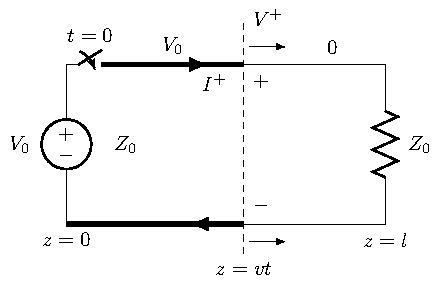
\includegraphics{figTransmissionLineTransientAtSwitchONWithMatchedLoadAndZeroGeneratorResistance}
\caption{ترسیلی تار میں ابتدائی موج۔}
\label{شکل_ترسیلی_ابتدائی_موج}
\end{figure}

آئیں اب برقی بوجھ کی قیمت اور ترسیلی تار کی قدرتی رکاوٹ برابر نہ رکھتے ہوئے مسئلے پر دوبارہ غور کریں۔ شکل \حوالہ{شکل_ترسیلی_عمومی_بار_ابتدائی_موج} میں ایسا ہی دور دکھایا گیا ہے جس میں منبع کی داخلی رکاوٹ بھی شامل کی گئی ہے۔لمحہ \عددی{t=0} پر سوئچ کو چالو حالت کر دیا جاتا ہے جس سے ترسیلی تار کے داخلی سرے پر \عددی{V_1=\tfrac{Z_0 V_0}{Z_0+R_g}} برقی دباو نمودار ہو گا۔یہ برقی دباو بطور موج \عددی{V_1^+} 
\begin{align}\label{مساوات_ترسیلی_عارضی_پہلی}
V_1^+=\frac{Z_0 V_0}{Z_0+Z_g}
\end{align}
برقی بوجھ کی جانب حرکت کرے گی۔
\begin{figure}
\centering
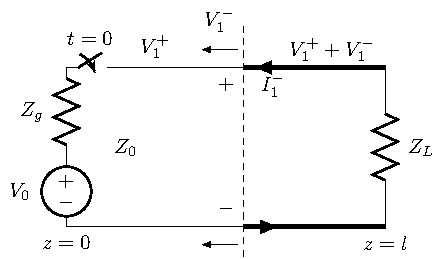
\includegraphics{figTransmissionLineTransientAtSwitchON}
\caption{عمومی برقی بوجھ سے لدے ترسیلی تار میں ابتدائی موج۔}
\label{شکل_ترسیلی_عمومی_بار_ابتدائی_موج}
\end{figure}

تار کے اختتام پر \عددی{Z_0 \ne Z_L} کی وجہ سے انعکاسی موج \عددی{V_1^-} پیدا ہو گی جہاں
\begin{align*}
\frac{V_1^-}{V_1^+}=\Gamma_L=\frac{Z_L-Z_0}{Z_L+Z_0}
\end{align*}
 کے برابر ہے۔انعکاسی موج برقی بوجھ سے منبع کی جانب حرکت کرتی ہے۔اس موج سے منبع کی جانب \عددی{V_1^+} برقی دباو پایا جاتا ہے جبکہ دوسری جانب \عددی{{V_1^+ + V_1^-}} برقی دباو ہو گا۔انعکاسی موج \عددی{V_1^-} منبع پر پہنچ کر دو رتبی منعکس موج \عددی{V_2^+} پیدا کرے گی جہاں
\begin{align*}
\frac{V_2^+}{V_1^-}=\Gamma_g=\frac{Z_g-Z_0}{Z_g+Z_0}
\end{align*}
کے برابر ہے۔اس کو
\begin{align*}
V_2^+=\Gamma_g V_1^-=\Gamma_g \Gamma_L V_1^+
\end{align*}
لکھا جا سکتا ہے۔اب \عددی{V_2^+} موج جب برقی بوجھ تک پہنچے گی تو یہ \عددی{V_2^-}
\begin{align*}
V_2^-=\Gamma_L V_2^+
\end{align*}
 پیدا کرے گی۔

اسی ترتیب کو بار بار استعمال کرتے ہوئے کسی بھی لمحے پر عارضی صورت حال دریافت کیا جا سکتا ہے۔متعدد انعکاس کے بعد برقی بوجھ پر برقی دباو
\begin{align*}
V_L&=V_1^+ + V_1^- + V_2^+ + V_2^- + V_3^+ + V_3^- + \cdots\\
&=V_1^+ (1+\Gamma_L + \Gamma_g \Gamma_L + \Gamma_g \Gamma_L ^2+\Gamma_g^2 \Gamma_L^2+\Gamma_g^2 \Gamma_L^3\cdots )
\end{align*}
ہو گا جسے
\begin{align*}
V_L=V_1^+(1+\Gamma_L)(1+\Gamma_g \Gamma_L+\Gamma_g^2 \Gamma_L^2+\cdots)
\end{align*}
لکھا جا سکتا ہے۔آپ جانتے ہیں کہ \عددی{1+r+r^2+r^3+\cdots+r^{n-1}=\tfrac{1-r^n}{1-r}} کے برابر ہے۔یہی کلیہ مندرجہ بالا مساوات کے آخری قوسین پر لاگو کرتے ہوئے  لامحدود انعکاس کے بعد
\begin{align*}
\left. V_L \right|_{t \to \infty}=V_1^+\left(\frac{1+\Gamma_L}{1-\Gamma_g \Gamma_L}\right) 
\end{align*}
لکھا جا سکتا ہے جہاں لمبا دورانیہ  \عددی{t \to \infty} کی صورت میں  \عددی{n \to \infty} اور \عددی{\Gamma_g^n \Gamma_L^n \to 0} ہوں گے۔اس مساوات میں \عددی{\Gamma_g=\tfrac{Z_g-Z_0}{Z_g+Z_0}} اور \عددی{\Gamma_L=\tfrac{Z_L-Z_0}{Z_L+Z_0}} پر کرتے ہوئے مساوات \حوالہ{مساوات_ترسیلی_عارضی_پہلی} کے استعمال  سے
\begin{align*}
\left. V_L \right|_{t \to \infty}=\frac{Z_L V_0}{Z_g+Z_L}
\end{align*}
حاصل ہوتا ہے جو برقرار یکساں حالت کی صورت میں برقی بوجھ پر برقی دباو ہے۔یہی جواب کرخوف کے قانون سے بھی حاصل ہوتا ہے جس میں ترسیلی تار کی قدرتی رکاوٹ کا کوئی کردار نہیں پایا جاتا۔

آئیں اب شکل \حوالہ{شکل_ترسیلی_عمومی_بار_ابتدائی_موج} میں عارضی دورانیے  کے دوران ترسیلی تار پر \عددی{z=\tfrac{4 l}{5}} کے مقام پر  برقی دباو بالمقابل وقت کا خط کھینچتے ہیں۔اس شکل میں \عددی{Z_g}، \عددی{Z_L} اور \عددی{Z_0} کو حقیقی اعداد تصور کرتے ہیں۔اس کے ساتھ ساتھ \عددی{Z_g > Z_0} اور \عددی{Z_L > Z_0} تصور کیا گیا ہے۔یوں \عددی{\Gamma_g > 0} اور \عددی{\Gamma> 0} حاصل ہوتے ہیں۔شکل \حوالہ{شکل_ترسیلی_عارضی_برقی_دباو_بالمقابل_وقت} کو دیکھ کر آگے پڑھیں۔
\begin{figure}
\centering
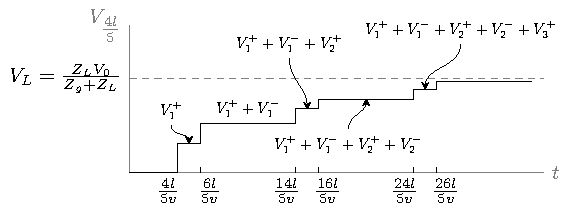
\includegraphics{figTransmissionLineTransientVoltageVersusTime}
\caption{عارضی دورانیے کی برقی دباو بالمقابل برقی دباو۔}
\label{شکل_ترسیلی_عارضی_برقی_دباو_بالمقابل_وقت}
\end{figure}

 سوئچ کو لمحہ \عددی{t=0} پر چالو حالت کیا جاتا ہے جس سے ترسیلی تار میں \عددی{V_1^+} موج پیدا ہوتی ہے۔یہ موج نقطہ دار لکیر سے ظاہر کردہ مقام تک \عددی{\tfrac{4l}{5v}} دورانیے میں پہنچتی ہے۔یوں \عددی{t=0} تا \عددی{t=\tfrac{4l}{5v}} اس نقطے پر صفر برقی دباو رہتا ہے جبکہ ٹھیک \عددی{t=\tfrac{4l}{5v}} پر یہاں کی برقی دباو \عددی{V_1^+} ہو جاتی ہے۔شکل \حوالہ{شکل_ترسیلی_عارضی_برقی_دباو_بالمقابل_وقت} میں ایسا ہوتا دکھایا گیا ہے۔موج \عددی{V_1^+} نقطہ دار لکیر سے برقی بوجھ تک \عددی{\tfrac{l}{5v}} دورانیے میں پہنچ کر انعکاس پذیر ہوتی ہے۔انعکاسی موج کو برقی بوجھ سے نقطہ دار لکیر تک پہنچنے کی خاطر \عددی{\tfrac{l}{5v}} دورانیہ درکار ہے۔یوں \عددی{V_1^-} موج نقطہ دار لکیر پر لمحہ \عددی{\tfrac{4l}{5v}+\tfrac{l}{5v}+\tfrac{l}{5v}=\tfrac{6l}{5v}} پہ پہنچتی ہے۔یوں سوئچ چالو حال کرنے کے \عددی{\tfrac{6l}{5v}} دیر بعد نقطہ دار لکیر پر برقی دباو \عددی{V_1^+ + V_1^-} ہو جاتی ہے۔امید کی جاتی ہے کہ آپ شکل \حوالہ{شکل_ترسیلی_عارضی_برقی_دباو_بالمقابل_وقت} میں دکھائے گئے تمام صورت حال کو سمجھ پائے ہیں۔آپ دیکھ سکتے ہیں کہ ترسیلی تار کے دونوں سروں پر موج بار بار انعکاس پذیر ہوتی ہے۔ہر انعکاس کے بعد برقی دباو برقرار حال قیمت کے قریب تر ہوتا جاتا ہے۔

ترسیلی تار پر کسی بھی مقام پر برقی رو کی قیمت بھی اسی طرح حاصل کی جاتی ہے۔برقی دباو کی صورت میں اس تار کو مثبت برقی دباو پر تصور کیا جاتا ہے جس پر مثبت بار پایا جاتا ہو۔یوں شکل \حوالہ{شکل_ترسیلی_عمومی_بار_ابتدائی_موج} میں \عددی{V_1^+} اور \عددی{V_1^-} امواج میں بالائی تار مثبت برقی دباو پر ہیں۔اسی شکل میں گھڑی کی سمت میں گھومتی برقی رو کو مثبت تصور کیا جاتا ہے جبکہ گھڑی کے الٹ سمت گھومتی برقی رو کو منفی تصور کیا جاتا ہے۔یوں \عددی{I_1^+} مثبت جبکہ \عددی{I_1^-} منفی برقی رو ہے۔یوں ترسیلی تار میں دونوں جانب حرکت کرتی برقی دباو کی موج کو مثبت تصور کیا جاتا ہے جبکہ برقی رو کے امواج مثبت یا منفی ممکن ہیں۔برقی رو اور برقی دباو کا عمومی تعلق
\begin{align*}
I_1^+&=\frac{V_1^+}{Z_0}\\
I_1^-&=-\frac{V_1^-}{Z_0}
\end{align*}
ہے۔اس طرح 
\begin{align*}
I_1^+&=\frac{V_1^+}{Z_0} , \quad \quad I_1^-=-\frac{V_1^-}{Z_0}\\
I_2^+&=\frac{V_2^+}{Z_0} , \quad \quad I_2^-=-\frac{V_2^-}{Z_0}\\
I_3^+&=\frac{V_3^+}{Z_0} , \quad \quad  I_3^-=-\frac{V_3^-}{Z_0}
\end{align*} 
لکھے جائیں گے۔

شکل \حوالہ{شکل_ترسیلی_عارضی_برقی_دباو_بالمقابل_وقت} کو دیکھتے ہوئے شکل \حوالہ{شکل_ترسیلی_عارضی_برقی_رو_بالمقابل_وقت} حاصل کیا گیا ہے۔اس شکل میں یہ دلچسپ حقیقت  سامنے آتی ہے کہ سوئچ چالو کرنے کے لمحے پر برقی رو برقرار حالت یکساں برقی رو سے زیادہ ہے۔دراصل \عددی{Z_g}، \عددی{Z_L} اور \عددی{Z_0} کی ایسی قیمتیں چنی جا سکتی ہیں کہ ابتدائی برقی دباو یا ابتدائی برقی رو کی قیمت برقرار حالت قیمتوں سے زیادہ یا کم ہو۔
\begin{figure}
\centering
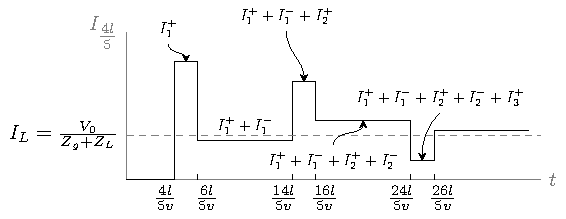
\includegraphics{figTransmissionLineTransientCurrentVersusTime}
\caption{عارضی دورانیے کی برقی رو بالمقابل برقی دباو۔}
\label{شکل_ترسیلی_عارضی_برقی_رو_بالمقابل_وقت}
\end{figure}

%===================
\ابتدا{مثال}
شکل \حوالہ{شکل_ترسیلی_عمومی_بار_ابتدائی_موج} میں \عددی{l=\SI{240}{\meter}}، \عددی{v=0.8 c}، \عددی{V_0=\SI{5}{\volt}}، \عددی{Z_L=\SI{100}{\ohm}}، \عددی{Z_g=\SI{50}{\ohm}} اور \عددی{Z_0=\SI{50}{\ohm}} ہیں۔سوئچ کو \عددی{t=0} پر چالو حالت میں کر دیا جاتا ہے۔عارضی دورانیے میں برقی بوجھ اور منبع  پر برقی دباو بالمقابل وقت اور  برقی رو بالمقابل وقت کے خط کھینچیں۔

حل:ان قیمتوں سے شرح انعکاس
\begin{align*}
\Gamma_g&=\frac{50-50}{50+50}=0\\
\Gamma_L&=\frac{100-50}{100+50}=\frac{1}{3}
\end{align*}
حاصل ہوتے ہیں۔لمحہ \عددی{t=0} پر سوئچ چالو کرنے سے منبع کو \عددی{Z_0} نظر آتا ہے لہٰذا
\begin{align*}
V_1^+&=\frac{Z_0 V_0}{Z_g+Z_0}=\frac{50 \times 5}{50+50}=\frac{5}{2} \, \si{\volt}\\
I_1^+&=\frac{V_0}{Z_g+Z_0}=\frac{5}{50+50}=\frac{1}{20} \, \si{\ampere}
\end{align*}
ہوں گے۔ترسیلی تار میں رفتار موج \عددی{v=0.8 \times 3 \times 10^8=\SI{2.4e8}{\meter\per\second}} ہے لہٰذا یہ امواج 
\begin{align*}
t=\frac{l}{v}=\frac{240}{2.4 \times 10^8}=\SI{1}{\micro\second}
\end{align*}
دورانیے میں برقی بوجھ تک پہنچیں گی۔برقی بوجھ سے انعکاس پذیر امواج
\begin{align*}
V_1^-&=\Gamma_L V_1^+=\frac{1}{3} \times \frac{5}{2}=\frac{5}{6} \, \si{\volt}\\
I_1^-&=-\frac{V_1^-}{Z_0}=-\frac{1}{60} \, \si{\ampere}
\end{align*}
ہیں۔یوں سوئچ چالو کرنے کے \عددی{\SI{1}{\micro\second}} دیر بعد برقی بوجھ پر کل برقی دباو اور برقی رو 
\begin{align*}
V_1^+ + V_1^- &=\frac{5}{2}+\frac{5}{6}=\frac{10}{3} \, \si{\volt}\\
I_1^+ + I_1^-&=\frac{1}{20}-\frac{1}{60}=\frac{1}{30} \, \si{\ampere}
\end{align*}
ہوں گے۔سوئچ چالو کرنے کے \عددی{\SI{2}{\micro\second}} دیر بعد انعکاسی امواج منبع تک واپس پہنچیں گی۔چونکہ \عددی{\Gamma_g=0} ہے لہٰذا منبع سے کوئی موج انعکاس پذیر نہیں ہو گی۔اس طرح سوئچ چالو کرنے کے \عددی{\SI{2}{\micro\second}} دیر بعد منبع پر برقی دباو اور برقی رو مندرجہ بالا قیمتیں اختیار کر لیں گے۔اس کے بعد یہی قیمتیں برقرار رہیں گے۔
\begin{figure}
\centering
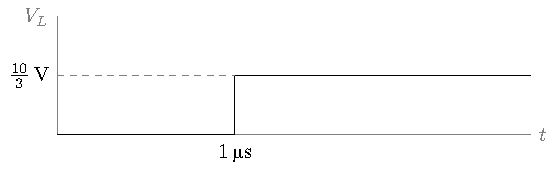
\includegraphics{figTransmissionLineTransientLoadVoltageVersusTimeExampleA}
\caption{برقی بوجھ پر برقی دباو۔}
\label{شکل_ترسیلی_مثال_بار_دباو}
\end{figure}
%
\begin{figure}
\centering
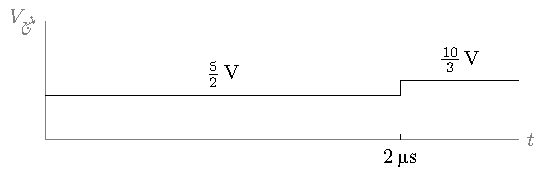
\includegraphics{figTransmissionLineTransientGeneratorTerminalVoltageVersusTimeExampleA}
\caption{منبع کے خارجی سروں پر برقی دباو۔}
\label{شکل_ترسیلی_مثال_منبع_دباو}
\end{figure}
%
\begin{figure}
\centering
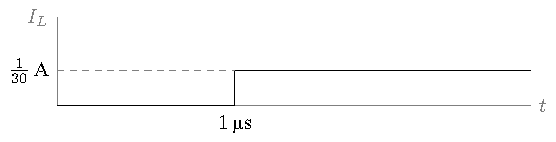
\includegraphics{figTransmissionLineTransientLoadCurrentVersusTimeExampleA}
\caption{برقی بوجھ کی برقی رو۔}
\label{شکل_ترسیلی_مثال_بار_رو}
\end{figure}
%
\begin{figure}
\centering
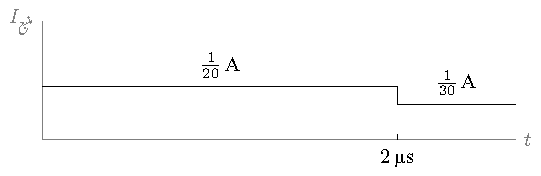
\includegraphics{figTransmissionLineTransientGeneratorCurrentVersusTimeExampleA}
\caption{منبع کی برقی رو۔}
\label{شکل_ترسیلی_مثال_منبع_رو}
\end{figure}
\انتہا{مثال}
%=============================

عارضی دورانیے کا ایک اہم مسئلہ شکل \حوالہ{شکل_ترسیلی_مستطیل_اشارہ} میں دکھایا گیا ہے جہاں \عددی{z=0} پر برقی بوجھ \عددی{R_L} جوڑا جا سکتا ہے جبکہ \عددی{z=l} پر تار کا سرا کھلا رکھا جاتا ہے۔بار بردار تار پر \عددی{V_0} مثبت برقی دباو پایا جاتا ہے جبکہ تار کی قدرتی رکاوٹ \عددی{Z_0} ہے۔آئیں اس کی کارکردگی پر غور کریں۔  
\begin{figure}
\centering
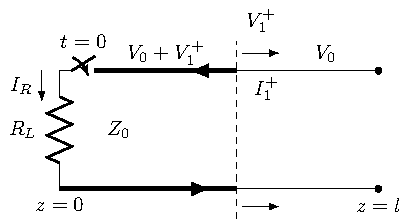
\includegraphics{figTransmissionLinePulseFormingNetwork}
\caption{ترسیلی تار سے مستطیل پتلا اشارہ حاصل کیا جا سکتا ہے۔}
\label{شکل_ترسیلی_مستطیل_اشارہ}
\end{figure}
سوئچ چالو کرتے ہی تار سے  بار کا انخلا بہ راستہ \عددی{R_L} شروع ہو جاتا ہے۔تار میں کثافت بار کی کمی سے تار میں برقی دباو کم ہوتا ہے۔ شکل \حوالہ{شکل_ترسیلی_مستطیل_اشارہ} میں سوئچ بند کرنے کے کچھ ہی دیر بعد کی صورت حال دکھائی گئی ہے۔سوئچ چالو کرنے سے پیدا موج کا مقام نقطہ دار لکیر  دکھا رہی ہے۔اس لکیر کے دائیں جانب برقی دباو \عددی{V_0} اور بار ساکن ہے جبکہ لکیر کے بائیں جانب بار حرکت میں ہے اور برقی دباو \عددی{V_0 + V_1^+} ہے۔چونکہ نقطہ دار لکیر کے بائیں جانب تار پر کثافت بار کم ہے لہٰذا اس طرف برقی دباو بھی کم ہو گا، جس سے صاف ظاہر ہے کہ \عددی{V_1^+} کی قیمت منفی ہو گی۔ نقطہ دار لکیر کے دائیں جانب برقی رو صفر کے برابر ہے جبکہ لکیر کے بائیں جانب برقی رو پائی جاتی ہے۔یہ برقی رو گھڑی کی الٹ سمت ہے لہٰذا تار میں ابتدائی برقی رو کی موج \عددی{I_1^+} کی قیمت منفی ہو گی۔برقی دباو کی موج \عددی{V_1^+} اور برقی رو کی موج \عددی{I_1^+}  ترسیلی تار میں \عددی{z=0} سے \عددی{z=l} جانب حرکت کرتی ہے۔ترسیلی تار میں برقی دباو اور برقی رو ہر صورت 
\begin{align*}
-I_R=I_1^+=\frac{V_1^+}{Z_0}
\end{align*}
مساوات پر پورا اترتے ہیں۔مزاحمت \عددی{R_L} پر برقی دباو \عددی{V_0 + V_1^+} ہے جو \عددی{I_R} کی وجہ سے ہے۔یوں برقی بوجھ پر \عددی{V_L=I_R R_L} ہو گا جسے
\begin{align*}
V_L=V_0 +V_1^+ =-I_1^+ R_L=-\frac{V_1^+}{Z_0} R_L
\end{align*}
لکھا جا سکتا ہے۔اس مساوات سے
\begin{align}\label{مساوات_ترسیلی_ابتدائی_برقی_مستطیل_اشارہ}
V_1^+=-\frac{Z_0 V_0}{Z_0+R_L}
\end{align}
حاصل ہوتا ہے۔برقی دباو کی ابتدائی موج جانتے ہوئے ہم کسی بھی لمحے کسی بھی نقطے پر برقی دباو یا برقی رو حاصل کر سکتے ہیں۔ایسا ہم کئی مرتبہ کر چکے ہیں۔

زیادہ دلچسپ صورت حال اس وقت پیدا ہوتی ہے جب \عددی{R_L=Z_0} ہو۔ایسی صورت میں ترسیلی تار کے سروں پر شرح انعکاس
\begin{align*}
\Gamma_{z=0}=0\\
\Gamma_{z=l}=1
\end{align*}
حاصل ہوتے ہیں جہاں \عددی{z=l} پر تار کا سرا کھلے دور ہے۔مساوات \حوالہ{مساوات_ترسیلی_ابتدائی_برقی_مستطیل_اشارہ} سے
\begin{align*}
V_1^+=-\frac{V_0}{2}
\end{align*}
حاصل ہوتا ہے۔یوں سوئچ چالو کرتے ہی برقی بوجھ پر دباو \عددی{V_L=V_0+V_1^+=\tfrac{V_0}{2}} پیدا ہوتا ہے۔موج \عددی{V_1^+} کو تار کے دائیں سرے تک پہنچنے کی خاطر \عددی{\tfrac{l}{v}} وقت درکار ہے جہاں سے یہ انعکاس پذیر ہو گی۔اس طرح سوئچ چالو کرنے کے ٹھیک \عددی{\tfrac{2l}{v}} دیر بعد منعکس برقی موج برقی  بوجھ پہنچ کر اس پر کل برقی دباو کی قیمت \عددی{\SI{0}{\volt}} کر دے گی۔چونکہ \عددی{R_L=Z_0} ہے لہٰذا  بوجھ سے موج انعکاس پذیر نہیں ہو گی۔برقی  بوجھ پر برقی دباو کو شکل \حوالہ{شکل_ترسیلی_تار_سے_حاصل_مستطیل_اشارہ} میں دکھایا گیا ہے۔آپ دیکھ سکتے ہیں کہ برقی بوجھ پر بالکل مستطیل برقی دباو پائی جاتی ہے۔انتہائی کم دورانیے کے مستطیل اشارات ترسیلی تار کی مدد سے پیدا کئے جا سکتے ہیں۔\عددی{R_L \ne Z_0} کی صورت میں موج کئی مرتبہ انعکاس پذیر ہو گی جس سے اشارہ مستطیل شکل کھو دے گا۔
\begin{figure}
\centering
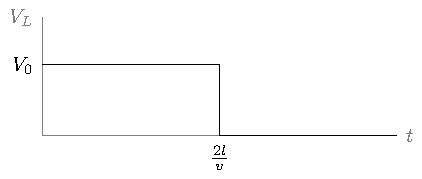
\includegraphics{figTransmissionLinePulse}
\caption{ترسیلی تار سے حاصل مستطیل پتلا اشارہ۔}
\label{شکل_ترسیلی_تار_سے_حاصل_مستطیل_اشارہ}
\end{figure}


%====================
\ابتدا{مثال}
\عددی{\SI{300}{\ohm}} کے برقی بوجھ پر \عددی{\SI{5000}{\volt}} اور \عددی{\SI{100}{\nano\second}} دورانیے کا مستطیل اشارہ درکار ہے۔اس اشارے کو \عددی{\SI{300}{\ohm}} کے ہم محوری تار سے حاصل کریں جہاں تار میں موج کی رفتار \عددی{0.8c} ہے۔
\begin{figure}
\centering
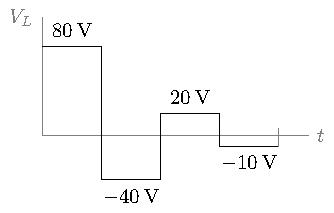
\includegraphics{figTransmissionLineTransientLoadVoltageVersusTimeExampleB}
\caption{بار بار انعکاس پذیر موج سے پیدا برقی دباو۔}
\label{شکل_ترسیلی_تار_بار_بار_انعکاس}
\end{figure}

حل:اشارے کے دورانیے سے تار کی لمبائی
\begin{align*}
l=\frac{0.8 \times 3 \times 10^8 \times 100 \times 10^{-9}}{2}=\SI{12}{\meter}
\end{align*}
حاصل ہوتی ہے۔ہم محوری تار کو \عددی{\SI{10}{\kilo \volt}} برقی دباو پر رکھتے ہوئے درکار اشارہ حاصل ہو گا۔
\انتہا{مثال}
%===================================
 \ابتدا{مثال}
شکل \حوالہ{شکل_ترسیلی_مستطیل_اشارہ} میں \عددی{V_0=\SI{320}{\volt}}،  \عددی{Z_0=\SI{50}{\ohm}} جبکہ \عددی{R_L=\tfrac{50}{3} \, \si{\ohm}} ہیں۔لمحہ \عددی{t=0} پر سوئچ کو چالو کیا جاتا ہے۔\عددی{0<t<\tfrac{8l}{v}} کے لئے مزاحمت پر برقی دباو حاصل کریں۔

حل:اس دورانیے میں موج ترسیلی تار میں چار چکر کاٹے گی۔دی گئی معلومات سے
\begin{align*}
\Gamma_{z=0}&=\frac{\frac{50}{3}-50}{\frac{50}{3}+50}=-\frac{1}{2}\\
\Gamma_{z=l}&=\frac{\infty - 50}{\infty + 50}=1
\end{align*}
حاصل ہوتے ہیں۔یوں
\begin{align*}
V_1^+&=-\frac{50 \times 320}{50+\frac{50}{3}}=\SI{-240}{\volt}\\
V_1^-&=\Gamma_{z=l} V_1^+=\SI{-240}{\volt}
\end{align*}
ہوں گے۔اسی طرح
\begin{align*}
V_2^+&=V_2^-=\Gamma_{z=0} V_1^-=\SI{120}{\volt}\\
V_3^+&=V_3^-=\Gamma_{z=0} V_2^-=\SI{-60}{\volt}\\
V_4^+&=V_4^-=\Gamma_{z=0} V_3^-=\SI{30}{\volt}\\
\end{align*}
حاصل ہوتے ہیں۔ان نتائج کو استعمال کرتے ہوئے
\begin{align*}
V_L&=V_0+V_1^+=320-240=\SI{80}{\volt} & (0<t<\tfrac{2l}{v})\\
&=V_0+V_1^+ +V_1^-+V_2^+=\SI{-40}{\volt} & (\tfrac{2l}{v}<t<\tfrac{4l}{v})\\
&=V_0+V_1^+ +V_1^-+V_2^+ +V_2^-+V_3^+=\SI{20}{\volt} & (\tfrac{4l}{v}<t<\tfrac{6l}{v})\\
&=V_0+V_1^+ +V_1^-+V_2^+ +V_2^-+V_3^+ +V_3^-+V_4^+=\SI{-10}{\volt} &  (\tfrac{6l}{v}<t<\tfrac{8l}{v})\\
\end{align*}
لکھا جا سکتا ہے۔ان نتائج کو شکل \حوالہ{شکل_ترسیلی_تار_بار_بار_انعکاس} میں دکھایا گیا ہے۔

\انتہا{مثال}
%===================================
\ابتدا{مثال}\شناخت{مثال_ترسیلی_سوئچ_تار_کے_درمیان}
شکل \حوالہ{شکل_ترسیلی_مثال_سوئچ_درمیان}-الف میں ترسیلی تار کے عین درمیان  \عددی{z=\tfrac{l}{2}} پر سوئچ نسب ہے جسے لمحہ \عددی{t=0} پر چالو کیا جاتا ہے۔اس دور میں \عددی{R_L=Z_0} ہے جبکہ منبع کی اندرونی مزاحمت \عددی{\SI{0}{\ohm}} کے برابر ہے۔برقی بوجھ پر برقی دباو کا خط کھینچیں۔
\begin{figure}
\centering
\begin{subfigure}{0.8\textwidth}
\centering
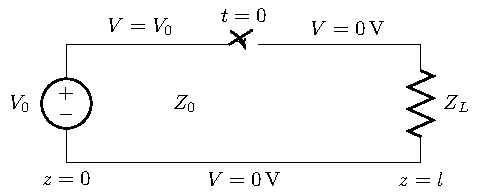
\includegraphics{figTransmissionLineTransientSwitchAtLineMid}
\caption{ترسیلی تار کے عین درمیانے نقطے پر سوئچ کو چالو کیا جاتا ہے۔}
\end{subfigure}

\begin{subfigure}{0.8\textwidth}
\centering
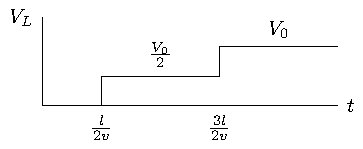
\includegraphics{figTransmissionLineTransientSwitchAtLineMidVoltageWave}
\caption{برقی بوجھ پر برقی دباو۔}
\end{subfigure}
\caption{مثال \حوالہ{مثال_ترسیلی_سوئچ_تار_کے_درمیان} کا دور اور اس میں برقی بوجھ پر برقی دباو۔}
\label{شکل_ترسیلی_مثال_سوئچ_درمیان}
\end{figure}

حل:سوئچ سے برقی بوجھ کی جانب ترسیلی تار پر \عددی{\SI{0}{\volt}} برقی دباو ہے جبکہ سوئچ سے منبع کی جانب ترسیلی تار بار بردار ہے جس سے اس جانب کی برقی دباو \عددی{V_0} ہے۔سوئچ چالو کرنے سے  دو برقی موج، سوئچ کے مقام پر،  پیدا ہوتی ہیں۔سوئچ سے برقی بوجھ  کی جانب موج کا حیطہ \عددی{\tfrac{V_0}{2}} جبکہ سوئچ سے منبع کی جانب موج کا حیطہ \عددی{-\tfrac{V_0}{2}} ہو گا۔چونکہ \عددی{R_L=Z_0} ہے لہٰذا برقی بوجھ پر انعکاسی موج پیدا نہیں ہو گی۔اس کے برعکس منبع پر \عددی{\Gamma_g=-1} کی بنا پر یہاں سے انعکاس ہو گا۔ان تمام کو مد نظر رکھتے ہوئے ہم لکھ سکتے ہیں۔
\begin{align*}
V_L&=0  &(0<t<\tfrac{l}{2v})\\
&=\frac{V_0}{2} & (\tfrac{l}{2v} < t < \tfrac{3l}{2v})\\
&=V_0 & (\tfrac{3l}{2v} < t  )
\end{align*}
ان نتائج کو شکل \حوالہ{شکل_ترسیلی_مثال_سوئچ_درمیان}-ب میں دکھایا گیا ہے۔

\انتہا{مثال}
%=====================================
\ابتدا{مثال}\شناخت{مثال_ترسیلی_دو_عدد_سوئچ}
شکل \حوالہ{شکل_ترسیلی_مثال_دو_سوئچ} میں ترسیلی تار میں دو عدد سوئچ نسب ہیں۔دونوں سوئچ کو لمحہ \عددی{t=0} پر بیک وقت چالو کیا جاتا ہے۔\عددی{Z_0=R_L} کی صورت میں برقی بوجھ پر برقی دباو کا خط کھینچیں۔
\begin{figure}
\centering
\begin{subfigure}{0.8\textwidth}
\centering
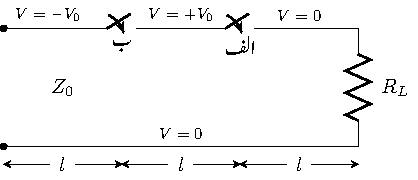
\includegraphics{figTransmissionLineTransientTwoSwitches}
\caption{ترسیلی تار میں دو سوئچ بیک وقت چالو کئے جاتے ہیں۔}
\end{subfigure}

\begin{subfigure}{0.8\textwidth}
\centering
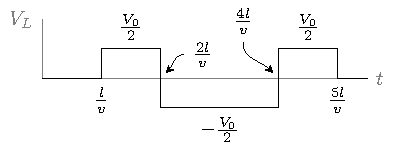
\includegraphics{figTransmissionLineTransientTwoSwitchVoltageWave}
\caption{برقی بوجھ پر عارضی دورانیے  میں برقی دباو کا خط۔}
\end{subfigure}
\caption{مثال \حوالہ{مثال_ترسیلی_دو_عدد_سوئچ} کا دور اور برقی بوجھ پر برقی دباو۔}
\label{شکل_ترسیلی_مثال_دو_سوئچ}
\end{figure}

حل:برقی بوجھ پر \عددی{\Gamma_L=0} ہے جبکہ ترسیلی تار کے کھلے سر پر \عددی{\Gamma=1} ہے۔دو سوئچ چالو کرنے سے کل چار عدد برقی دباو کی امواج پیدا ہوتی ہیں۔ان میں سے دو عدد موج برقی بوجھ کی جانب حرکت کرتے ہیں جبکہ بقایا دو عدد موج ترسیلی تار کے کھلے سر کی جانب حرکت کرتے ہیں۔کھلے سر پر دونوں امواج انعکاس پذیر ہو کر برقی بوجھ کی جانب لوٹتے ہیں۔برقی بوجھ سے کوئی موج انعکاس پذیر نہیں ہوتی۔

سوئچ-الف سے  برقی بوجھ جانب \عددی{\tfrac{V_0}{2}} وولٹ کی موج جبکہ کھلے سر کی جانب \عددی{-\tfrac{V_0}{2}} وولٹ کی موج حرکت کرتی ہے۔پہلی موج \عددی{t=\tfrac{l}{v}} دیر بعد برقی بوجھ تک پہنچتی ہے۔دوسری موج کھلے سر سے انعکاس پذیر ہو کر برقی بوجھ تک \عددی{t=\tfrac{5l}{v}} دورانیے میں پہنچتی ہے۔

سوئچ-ب سے برقی بوجھ جانب \عددی{-V_0} حیطے کی موج حرکت کرتے ہوئے برقی بوجھ تک \عددی{t=\tfrac{2l}{v}} دورانیے میں پہنچتی ہے جبکہ دوسری موج کا حیطہ \عددی{+V_0} ہے اور ترسیلی تار کے کھلے سر سے ہوتے ہوئے برقی بوجھ تک \عددی{\tfrac{4l}{v}} وقت میں پہنچتی ہے۔ان حقائق سے برقی بوجھ پر برقی دباو کا خط حاصل کیا جاتا ہے جسے شکل \حوالہ{شکل_ترسیلی_مثال_دو_سوئچ} میں دکھایا گیا ہے۔

\انتہا{مثال}
%======================
\begin{figure}
\centering
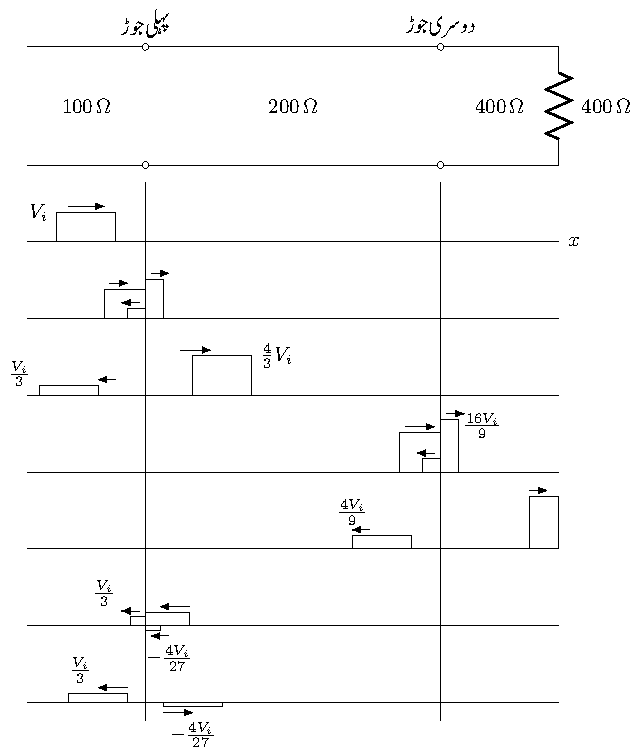
\includegraphics{figTransmissionLineWithMultipleJunctionsTranssientSinglePulse}
\caption{باریک اشارے کی انعکاس اور ترسیل۔}
\label{شکل_ترسیلی_تار_باریک_اشارے_کی_انعکاس}
\end{figure}
%====================

شکل \حوالہ{شکل_ترسیلی_تار_باریک_اشارے_کی_انعکاس} میں تین مختلف قدرتی رکاوٹ کے ترسیلی تاروں کو سلسلہ وار جوڑا گیا ہے جن کے آخر میں \عددی{\SI{400}{\ohm}} کی مزاحمت جڑی ہے۔بائیں جانب سے ایک عدد مستطیلی اشارہ مزاحمت کی طرف بڑھ رہا ہے۔ میں امید کرتا ہوں کہ آپ شکل میں دئے مختلف لمحات پر صورت حال سمجھ پائیں گے۔
\newpage
\حصہء{سوالات}

\ابتدا{سوال}
ترسیلی تار کے مستقل \عددی{R=\SI{20}{\ohm\per\meter}}، \عددی{L=\SI{4}{\micro\henry\per\meter}}، \عددی{G=\SI{80}{\micro\siemens\per\meter}} اور \عددی{C=\SI{60}{\pico\farad\per\meter}} ہیں۔اس میں \عددی{\SI{200}{\mega\hertz}} تعدد کی برقی موج حرکت کر رہی ہے۔ الف) \عددی{\gamma}، \عددی{\alpha}، \عددی{\beta}، \عددی{\lambda} اور \عددی{Z_0} حاصل کریں۔ب)  \عددی{\SI{12}{\meter}} فاصلہ طے کرنے کے بعد موج کا حیطہ ابتدائی قیمت کی نسبت سے کتنا ہو گا؟ پ) \عددی{\SI{1.6}{\meter}} فاصلہ طے کرنے کے بعد موج کا زاویائی فرق کتنا ہو گا؟ 

جوابات:\عددی{\gamma=0.049+j3.1 \, \si{\meter^{-1}}}، \عددی{\alpha=\SI{0.049}{\neper\per\meter}}، \عددی{\beta=\SI{3.1}{\radian\per\meter}}، \عددی{\lambda=\SI{2.03}{\meter}}، \عددی{Z_0=258-j2.37 \, \si{\ohm}}، \عددی{\SI{55.5}{\percent}}، \عددی{284^{\circ}}
\انتہا{سوال}
%==================
\ابتدا{سوال}
ایک ترسیلی تار جس میں موج کی رفتار \عددی{\SI{3e8}{\meter\per\second}} ہے کی قدرتی رکاوٹ \عددی{Z_0=\SI{50}{\ohm}} ہے۔ تار کے داخلی سروں پر \عددی{\SI{20}{\mega\hertz}} کی موج پیدا کی جا رہی ہے جبکہ اس کا دوسرا سرا قصر دور کیا گیا ہے۔ الف) تار کی لمبائی \عددی{\SI{3.75}{\meter}} ہونے کی صورت میں \عددی{Z_{\text{داخلی}}} حاصل کریں۔ ب) تار کی لمبائی بالترتیب \عددی{\SI{7.5}{\meter}}، \عددی{\SI{1.2}{\meter}} اور \عددی{\SI{9}{\meter}} ہونے کی صورت میں \عددی{Z_{\text{داخلی}}} حاصل کریں۔

جوابات:\عددی{\infty}، \عددی{\SI{0}{\ohm}}، \عددی{27.5j \, \si{\ohm}}، \عددی{36.3j \, \si{\ohm}} 
\انتہا{سوال}
%==================
\ابتدا{سوال}
بے ضیاع ترسیلی تار کی فی میٹر امالہ \عددی{\SI{0.25}{\micro\henry\per\meter}} جبکہ اس کی قدرتی رکاوٹ \عددی{\SI{75}{\ohm}} ہے۔الف) تار کی فی میٹر برقی گنجائش دریافت کریں۔ ب) تار میں موج کی رفتار حاصل کریں۔ پ) موج کی تعدد \عددی{\SI{50}{\mega\hertz}} ہونے کی صورت میں \عددی{\beta} حاصل کریں۔ ت) تار کے ساتھ \عددی{\SI{55}{\ohm}} کا برقی بوجھ منسلک ہے۔ \عددی{\Gamma} اور \عددی{s} حاصل کریں۔

جوابات:\عددی{\SI{44.4}{\pico\farad\per\meter}}، \عددی{\SI{3e8}{\meter\per\second}}، \عددی{\beta=\SI{1.05}{\radian\per\meter}}، \عددی{\Gamma=-\tfrac{2}{13}}، \عددی{s=\tfrac{15}{11}}
\انتہا{سوال}
%====================
\ابتدا{سوال}
ترسیلی تار کی قدرتی رکاوٹ \عددی{\SI{300}{\ohm}} ہے۔موج کی تعدد \عددی{\SI{6e8}{\radian\per\second}} جبکہ اس کی رفتار \عددی{\SI{2.8e8}{\meter\per\second}} ہے۔ الف) تار کی فی میٹر امالہ اور برقی گنجائش حاصل کریں۔ ب) تار پر سلسلہ وار جڑی \عددی{\SI{150}{\ohm}} اور \عددی{\SI{0.8}{\micro\henry}} کا برقی بوجھ ڈالا جاتا ہے۔ \عددی{\Gamma} اور \عددی{s} حاصل کریں۔

جوابات:\عددی{L=\SI{1.07}{\micro\henry\per\meter}}، \عددی{C=\SI{11.9}{\pico\farad\per\meter}}، \عددی{\Gamma=0.38+j0.67}، \عددی{s=7.49}
\انتہا{سوال}
%======================
\ابتدا{سوال}
بے ضیاع ترسیلی تار کی \عددی{\SI{80}{\mega\hertz}} تعدد پر قدرتی رکاوٹ \عددی{\SI{75}{\ohm}} اور \عددی{\beta=0.25 \pi \, \si{\radian\per\meter}} ہیں۔ الف) تار کی \عددی{L} اور \عددی{C} حاصل کریں۔ ب) تار پر \عددی{Z_L=80+j100 \, \si{\ohm}} برقی بوجھ لادا جاتا ہے۔برقی بوجھ سے کتنے فاصلے پر تار کی داخلی رکاوٹ \عددی{Z_{\text{داخلی}}} حقیقی  یعنی \عددی{Z_{\text{داخلی}}=R+j0} ہو گا۔

جوابات:\عددی{L=\SI{117}{\nano\henry\per\meter}}، \عددی{C=\SI{20.8}{\pico\farad\per\meter}}، \عددی{\SI{60.34}{\centi\meter}} 
\انتہا{سوال}
%======================
\ابتدا{سوال}
تعدد \عددی{\SI{1}{\mega\radian\per\second}} پر ضیاع کار ترسیلی تار کی قدرتی رکاوٹ  \عددی{Z_0=40+j0 \, \si{\ohm}} اور حرکی مستقل \عددی{\gamma=2+j6 \, \si{\meter^{-1}}} ہیں۔ الف) \عددی{G}، \عددی{C}، \عددی{R} اور \عددی{L} حاصل کریں۔

جوابات:\عددی{G=\SI{0.05}{\siemens\per\meter}}، \عددی{C=\SI{150}{\nano\farad\per\meter}}، \عددی{R=\SI{80}{\ohm\per\meter}}، \عددی{L=\SI{0.24}{\milli\henry\per\meter}}
\انتہا{سوال}
%======================
\ابتدا{سوال}
بے ضیاع ترسیلی تار کی \عددی{\SI{150}{\mega\hertz}} تعدد پر \عددی{Z_0=\SI{80}{\ohm}} اور \عددی{\beta=\SI{6}{\radian\per\meter}} ہیں۔تار پر متوازی جڑے \عددی{\SI{200}{\ohm}} کی مزاحمت اور \عددی{\SI{10}{\pico\farad}} کی برق گیر (کپیسٹر)  کا برقی بوجھ لادا جاتا ہے۔ الف) \عددی{L} اور \عددی{C} حاصل کریں۔ ب) شرح ساکن موج حاصل کریں۔

جوابات:\عددی{L=\SI{0.51}{\micro\henry\per\meter}}، \عددی{C=\SI{79.6}{\pico\farad\per\meter}}، \عددی{s=4.07}
\انتہا{سوال}
%=====================
\ابتدا{سوال}
منبع برقی دباو سلسلہ وار جڑی رکاوٹ \عددی{Z=300-j300 \, \si{\ohm}} اور بے ضیاع ترسیلی تار کے ساتھ منسلک ہے۔ترسیلی تار کا دوسرا سرا کسے دور ہے۔ترسیلی تار میں طول موج \عددی{\lambda} ہے۔ الف) منبع برقی دباو پر کل \عددی{\SI{300}{\ohm}} رکاوٹ مہیا کرنے کی خاطر ترسیلی تار کی لمبائی کتنی رکھی جائے گی۔ ب) ترسیلی تار کی لمبائی کے  تمام ممکنہ جواب حاصل کریں۔

جوابات:\عددی{\text{لمبائی}=\tfrac{\lambda}{8}}، \عددی{\text{لمبائی}=\tfrac{\lambda}{8}+\tfrac{m \lambda}{2}}
\انتہا{سوال}
%========================
\ابتدا{سوال}
تعدد \عددی{\SI{50}{\mega\hertz}} کے منبع برقی دباو کے ساتھ رکاوٹ \عددی{Z_g=50+j50 \, \si{\ohm}} اور بے ضیاع ترسیلی تار سلسلہ وار جڑے ہیں۔ ترسیلی تار کی قدرتی رکاوٹ \عددی{Z_0=\SI{100}{\ohm}}، لمبائی \عددی{\tfrac{\lambda}{4}} ہے اور یہ برقی بوجھ \عددی{Z_L} کو طاقت فراہم کر رہی ہے۔ الف) برقی بوجھ کی وہ قیمت دریافت کریں جس پر منبع برقی دباو کو کل \عددی{\SI{100}{\ohm}} رکاوٹ نظر آتی ہے۔ ب) ترسیلی تار کی فی میٹر امالہ \عددی{L=\SI{1.5}{\micro\henry\per\meter}} ہونے کی صورت میں ترسیلی تار میں موج کی رفتار اور ترسیلی تار کی لمبائی دریافت کریں۔ 

جوابات:\عددی{Z_L=100+j100 \, \si{\ohm}}، \عددی{\SI{6.6737}{\meter\per\second}}، \عددی{\SI{0.333}{\meter}}
\انتہا{سوال}
%=======================
\ابتدا{سوال}
تیس میٹر لمبی بے ضیاع ترسیلی تار کے دونوں سرے آزاد رکھنے کی صورت میں اس کی کل برقی گنجائش \عددی{C=\SI{1.5}{\nano\farad}} ناپی جاتی ہے۔اس کا ایک سرا قصر دور کرتے ہوئے دوسرے سرے پر نہایت کم دورانیے کا مستطیلی برقی دباو کا جھٹکا دیا جاتا ہے جو قصر دور سرے سے ٹکرا کر واپس لوٹتا ہے۔تار میں دو طرفہ فاصلہ کل \عددی{\SI{0.4}{\micro\second}} میں طے پاتا ہے۔ترسیلی تار کی قدرتی رکاوٹ حاصل کریں۔

جواب:\عددی{Z_0=\SI{133.3}{\ohm}}  
\انتہا{سوال}
%=======================
\ابتدا{سوال}
ترسیلی تار کی قدرتی رکاوٹ \عددی{Z_0=\SI{60}{\ohm}} جبکہ اس پر موج کی رفتار \عددی{\SI{2.8e8}{\meter\per\second}} ہے۔تار پر آمدی موج کی مساوات درج ذیل ہے۔
\begin{align*}
V_s^{+}(z,t)=100 \cos(\omega t -\pi z) \quad \quad  \si{\volt}
\end{align*}
 الف) موج کی زاویائی تعدد حاصل کریں۔ ب) آمدی برقی رو کی موج کی مساوات لکھیں۔ پ) ترسیلی تار کا \عددی{z>0} حصہ ہٹا کر \عددی{z=0} پر \عددی{Z_L=60+j40\,\si{\ohm}} رکاوٹ نسب کرنے کی صورت میں \عددی{\Gamma} حاصل کریں۔انعکاسی موج \عددی{V_s^{-}(z,t)} کی مساوات لکھیں اور \عددی{z=\SI{-2.25}{\meter}} پر \عددی{V_s} حاصل کریں۔

جوابات:\عددی{\omega=\SI{879.6}{\mega \radian\per\second}}، \عددی{I^+(z,t)=\tfrac{5}{3}\cos(\omega t -\pi z) \, \si{\ampere}}،
 \عددی{\Gamma=0.1+j0.3= 0.316 \phase{71.6^{\circ}}}، \\
\عددی{V_s^{-}(z,t)=31.6 e^{j(\pi z+1.249)} \, \si{\volt}}، \عددی{V_s(z=\SI{-2.5}{\meter})=130.4 e^{j 0.71} =130.4\phase{40.6^{\circ}}}
\انتہا{سوال}
%========================
\ابتدا{سوال}
ترسیلی تار کی \عددی{Z_0=\SI{50}{\ohm}}، لمبائی \عددی{\SI{330}{\meter}} اور اس میں رفتار موج \عددی{v=0.8 c} ہے۔یہ \عددی{Z_L=40+j70 \, \si{\ohm}} برقی بوجھ پر اختتام پذیر ہے۔تعدد \عددی{\SI{1.2}{\mega\hertz}} پر  \عددی{\Gamma}، \عددی{s} اور \عددی{Z_{\text{داخلی}}} حاصل کریں۔

جوابات:\عددی{0.62\phase{60.3^{\circ}}}، \عددی{4.27}، \عددی{100\phase{-56.2^{\circ}}}
\انتہا{سوال}
%=======================
\ابتدا{سوال}
بے ضیاع ترسیلی تار کی لمبائی \عددی{\SI{3}{\meter}}، قدرتی رکاوٹ \عددی{\SI{300}{\ohm}} جبکہ اس  پر طول موج \عددی{\SI{4}{\meter}} ہے۔ترسیلی تار کے ساتھ نسب برقی بوجھ \عددی{100-j 150 \,\si{\ohm}} پر \عددی{100\phase{30^{\circ}}} برقی دباو پایا جاتا ہے۔ الف) ترسیلی تار کے داخلی سرے پر برقی دباو حاصل کریں۔ ب) تار پر زیادہ سے زیادہ برقی دباو کیا پایا جائے گا؟

جوابات:\عددی{166.4 \phase{-63.7^{\circ}} \, \si{\volt}}، \عددی{\SI{187.8}{\volt}}
\انتہا{سوال}
%=======================
\ابتدا{سوال}
بے ضیاع ترسیلی تار کی لمبائی \عددی{\SI{38}{\meter}} ہے جبکہ اس کے مستقل \عددی{L=\SI{0.3}{\micro\henry\per\meter}} اور \عددی{C=\SI{90}{\pico\farad\per\meter}} ہیں۔برقی بوجھ \عددی{Z_L=40+j0 \, \si{\ohm}} ہے جبکہ داخلی جانب \عددی{\SI{4}{\mega\hertz}} تعدد کا منبع \عددی{200\phase{0^{\circ}} \, \si{\volt}} مہیا کر رہا ہے۔ الف) داخلی برقی رو کا حیطہ حاصل کریں۔ ب) برقی بوجھ پر برقی رو کا حیطہ حاصل کریں۔ پ) برقی بوجھ کو منتقل طاقت حاصل کریں۔

جوابات: \عددی{\SI{10.2}{\ampere}}، \عددی{\SI{3.52}{\ampere}}، \عددی{\SI{247.9}{\watt}}
\انتہا{سوال}
%========================
\ابتدا{سوال}
\عددی{\SI{300}{\ohm}} قدرتی رکاوٹ کی ترسیلی تار پر متوازی جڑے \عددی{\SI{400}{\ohm}} اور \عددی{\SI{600}{\ohm}} کا برقی بوجھ لادا جاتا ہے۔تار کی لمبائی \عددی{\tfrac{5 \lambda}{8}} ہے جبکہ اسے داخلی جانب \عددی{v(t)=310\cos(2\times 10^9 t) \, \si{\volt}} برقی دباو مہیا کی جاتی ہے۔برقی بوجھ سے لدے ترسیلی تار کی داخلی رکاوٹ \عددی{Z_{\text{داخلی}}} حاصل کرتے ہوئے  بالترتیب دونوں مزاحمتوں کو مہیا اوسط طاقت حاصل کریں۔

جوابات:\عددی{Z_{\text{داخلی}}=292.7+j65.9 \, \si{\ohm}}، \عددی{\SI{93.8}{\watt}}، \عددی{\SI{62.5}{\watt}}
\انتہا{سوال}
%========================
\ابتدا{سوال}
صفحہ \حوالہصفحہ{شکل_ترسیلی_تار_بار_بردار} پر شکل \حوالہ{شکل_ترسیلی_تار_بار_بردار}-الف میں برقی بوجھ کو ترسیلی تار کے ذریعہ منبع سے طاقت فراہم کرتا دکھایا گیا ہے۔موجودہ سوال میں \عددی{Z_0=\SI{60}{\ohm}}، برقی  بوجھ \عددی{Z_L=40-j50 \, \si{\ohm}}، منبع کی خارجی مزاحمت \عددی{Z_g=\SI{40}{\ohm}}، تعدد \عددی{\SI{e8}{\hertz}}، تار کی لمبائی \عددی{\SI{1.3}{\meter}} جبکہ منبع کی برقی دباو \عددی{80 \phase{0} \, \si{\volt}} ہیں۔ترسیلی تار میں موج کی رفتار \عددی{c} کے برابر ہے۔ الف) شرح ساکن موج \عددی{s} اور ترسیلی تار کی \عددی{Z_{\text{داخلی}}} حاصل کریں۔ ب)  \عددی{Z_g} اور \عددی{Z_L} میں اوسط طاقت ضیاع حاصل کریں۔  پ) ترسیلی تار میں طاقت کا ضیاع حاصل کریں۔   

جوابات: \عددی{s=2.86}، \عددی{Z_{\text{داخلی}}=99.1-j75.2 \, \si{\ohm}}، \عددی{\SI{5.1}{\watt}}، \عددی{\SI{12.7}{\watt}}، \عددی{\SI{0}{\watt}}
\انتہا{سوال}
%==========================
\ابتدا{سوال}
ترسیلی تار کی لمبائی \عددی{\tfrac{8\lambda}{7}}، قدرتی رکاوٹ \عددی{Z_0=\SI{75}{\ohm}} جبکہ اس پر برقی بوجھ \عددی{Z_L=100-j50} ہے۔تار میں موج کی رفتار \عددی{c} ہے۔اسے داخلی جانب \عددی{\SI{100}{\ohm}} کے خارجی مزاحمت کے منبع سے \عددی{600 \phase{0} \, \si{\volt}} برقی دباو مہیا کی جاتی ہے۔ الف) \عددی{\Gamma}، \عددی{s} اور \عددی{Z_{\text{داخلی}}} حاصل کریں۔ ب) ترسیلی تار کی داخلی برقی رو اور اسے مہیا طاقت حاصل کریں۔ پ)  برقی بوجھ پر برقی دباو اور اس کی برقی رو حاصل کریں۔ ت) برقی بوجھ کو منتقل طاقت حاصل کریں۔

جوابات:الف) \عددی{\Gamma=0.21-j0.23}، \عددی{s=1.89}، \عددی{Z_{\text{داخلی}}=41.7-j14 \, \si{\ohm}} ب) \عددی{4.2\phase{5.6^{\circ}} \, \si{\ampere}}، \عددی{\SI{370}{\watt}} پ) \عددی{304\phase{-63^{\circ}} \, \si{\volt}}، \عددی{2.7\phase{-37} \, \si{\ampere}} ت) \عددی{\SI{370}{\watt}}
\انتہا{سوال}
%=============================
\ابتدا{سوال}
قدرتی رکاوٹ \عددی{Z_0=\SI{300}{\ohm}} اور لمبائی \عددی{\SI{0.7}{\meter}} کے ترسیلی تار کا خارجی سرا قصر دور کیا جاتا ہے۔تار پر طول موج \عددی{\SI{0.34}{\meter}} ہے۔داخلی اشارے کا حیطہ \عددی{\SI{15}{\volt}} ہونے کی صورت میں تار پر زیادہ سے زیادہ حیطہ کیا پایا جائے گا؟ قصر دور سرے میں برقی رو کا حیطہ دریافت کریں۔

جوابات:\عددی{\SI{41.5}{\volt}}، \عددی{\SI{138.4}{\milli\ampere}}
\انتہا{سوال}
%===========================
\ابتدا{سوال}
منبع برقی رو \عددی{0.4\phase{0} \, \si{\ampere}} جس کی خارجی مزاحمت \عددی{\SI{80}{\ohm}} ہے، \عددی{3.4\lambda} لمبی ترسیلی تار کے ذریعہ \عددی{\SI{25}{\ohm}} کے برقی بوجھ کو طاقت فراہم کر رہی ہے۔ترسیلی تار کی قدرتی رکاوٹ \عددی{\SI{50}{\ohm}} ہے۔مزاحمتی برقی بوجھ اور منبع کی مزاحمت میں طاقت کا ضیاع دریافت کریں۔

جوابات:\عددی{\SI{1.28}{\watt}}، \عددی{\SI{0.81}{\watt}}
\انتہا{سوال}
%=========================

\ابتدا{سوال}
برقی بوجھ \عددی{Z_L=90-j55\,\si{\ohm}} کو \عددی{0.12\lambda} لمبائی اور \عددی{Z_0=\SI{70}{\ohm}} قدرتی رکاوٹ کی ترسیلی تار طاقت فراہم کرتی ہے۔سمتھ نقشہ استعمال کرتے ہوئے برقی بوجھ سے لدے  ترسیلی تار کی داخلی قدرتی رکاوٹ \عددی{Z_{\text{داخلی}}} اور شرح ساکن موج \عددی{s} حاصل کریں۔

جوابات:\عددی{38-j 20 \, \si{\ohm}}، \عددی{s=2.05}
\انتہا{سوال}
%============================
\ابتدا{سوال}
بے ضیاع ترسیلی تار کی قدرتی رکاوٹ \عددی{Z_0=\SI{400}{\ohm}}  ہے۔ تار کو \عددی{\SI{200}{\mega\hertz}} تعدد پر استعمال کیا جا رہا ہے۔اس
 تعدد پر \عددی{Z_{\text{داخلی}}=200-j200 \, \si{\ohm}} ہے۔تار کی لمبائی \عددی{\SI{1}{\meter}} ہے۔ سمتھ نقشہ استعمال کرتے ہوئے  الف) شرح ساکن موج حاصل کریں۔ ب) تار پر نسب برقی بوجھ \عددی{Z_L} حاصل کریں۔ پ) بلند تر برقی دباو کا مقام حاصل کریں۔

جوابات:\عددی{s=2.62}، \عددی{Z_L=1040+j69.8 \, \si{\ohm}}، \عددی{z=\SI{-7.2}{\milli\meter}}
\انتہا{سوال}
%===========================
\ابتدا{سوال}
بے ضیاع دو متوازی تار پر مبنی ترسیلی تار کی لمبائی \عددی{\SI{25}{\meter}}، قدرتی رکاوٹ \عددی{\SI{300}{\ohm}} اور فی میٹر برقی گنجائش \عددی{\SI{12}{\pico\farad\per\meter}} ہے۔نقطہ \عددی{z=0} پر تار کے ساتھ متوازی جڑے مزاحمت \عددی{\SI{800}{\ohm}} اور برقی گنجائش \عددی{\SI{5}{\pico\farad}} کا برقی بوجھ جڑا ہے۔تعدد \عددی{\omega=\SI{e10}{\radian\per\second}} پر سمتھ نقشے کے ذریعہ \عددی{\Gamma}، \عددی{s} اور \عددی{Z_{\text{داخلی}}} حاصل کریں۔

جوابات:\عددی{\Gamma=0.44-j0.16}، \عددی{s=2.7}، \عددی{Z_{\text{داخلی}}=584+j335 \, \si{\ohm}}
\انتہا{سوال}
%==========================
\ابتدا{سوال}
بے ضیاع ترسیلی تار پر \عددی{\tfrac{Z_L}{Z_0}=2+j1} جبکہ \عددی{\lambda=\SI{20}{\meter}} ہے۔سمتھ نقشے کے استعمال کرتے ہوئے حل کریں۔ الف) وہ نقطہ دریافت کریں جس پر \عددی{z_{\text{داخلی}}=r+j0} ہو جہاں \عددی{r>1} ہے۔ ب) اس نقطے پر \عددی{z_{\text{داخلی}}} حاصل کریں۔ پ) اس نقطے پر ترسیلی تار کو کاٹ کر برقی بوجھ جانب حصے کو ہٹایا جاتا ہے جبکہ نئے سرے پر  \عددی{r} نسب کیا جاتا ہے۔ترسیلی تار پر \عددی{s} حاصل کریں۔ ت) نسب کئے گئے \عددی{r} سے کتنے فاصلے پر \عددی{\tfrac{Z_L}{Z_0}=2+j1} ہو گا؟

جوابات:\عددی{\SI{0.74}{\meter}}، \عددی{z_{\text{داخلی}}=2.61+j0 \, \si{\ohm}}، \عددی{s=2.61}، \عددی{\SI{9.26}{\meter}}
\انتہا{سوال}
%==============================
\ابتدا{سوال}
ترسیلی تار پر \عددی{Z_L=25+j75 \, \si{\ohm}} برقی بوجھ  نقطہ  \عددی{z=0} پر جڑی ہے۔تار کی قدرتی رکاوٹ \عددی{Z_0=\SI{50}{\ohm}} اور اس پر موج کی رفتار \عددی{v=c} ہے۔برقی بوجھ کے قریبی اس نقطے کو دریافت کریں جس پر داخلی رکاوٹ کا حقیقی جزو \عددی{\tfrac{1}{Z_0}} کے برابر ہو جبکہ اس کا خیالی جزو منفی قیمت رکھتا ہو۔اس نقطے پر 
\عددی{y_{\text{داخلی}}} حاصل کریں۔اس نقطے پر کتنا برق گیر (کپیسٹر)  نسب کرنے سے بقایا تار پر \عددی{s=1} حاصل ہو گا؟ 

جوابات:\عددی{\SI{39.6}{\centi\meter}}، \عددی{y_{\text{داخلی}}=1-j2.23}، \عددی{C=\SI{24}{\pico\farad}}
\انتہا{سوال}
%==============================
\ابتدا{سوال}\شناخت{سوال_ترسیلی_بار_بردار_الف}
صفحہ \حوالہصفحہ{شکل_ترسیلی_عمومی_بار_ابتدائی_موج} میں شکل \حوالہ{شکل_ترسیلی_عمومی_بار_ابتدائی_موج} دکھایا گیا ہے۔اس میں \عددی{Z_0=\SI{50}{\ohm}}، \عددی{R_g=R_L=\SI{25}{\ohm}} جبکہ منبع کی برقی دباو \عددی{V_0} ہے۔ لمحہ \عددی{t=0} پر سوئچ چالو کیا جاتا ہے۔\عددی{0<t<\tfrac{8l}{v}} دورانیے کے لئے برقی بوجھ  کی برقی دباو اور  منبع کی برقی رو کے خط کھینچیں۔

\begin{figure}
\centering
\begin{subfigure}{0.9\textwidth}
\centering
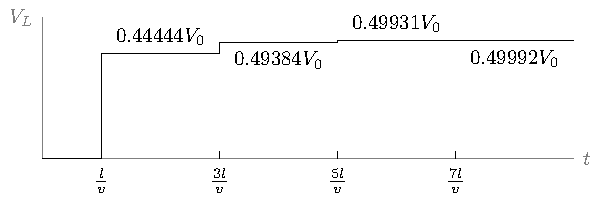
\includegraphics{figTransmissionLineTransientLoadVoltageQuestionA}
\caption{ برقی بوجھ کی برقی دباو بالمقابل وقت۔}
\label{شکل_ترسیلی_جواب_سوال_الف}
\end{subfigure}%

\begin{subfigure}{0.9\textwidth}
\centering
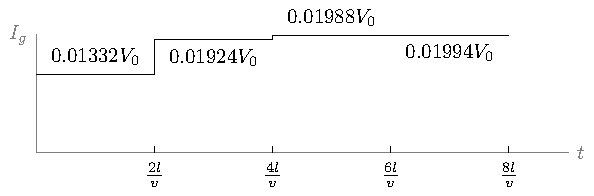
\includegraphics{figTransmissionLineTransientSourceCurrentQuestionA}
\caption{منبع کی برقی رو بالمقابل وقت۔}
\label{شکل_ترسیلی_جواب_منبع_رو_سوال_الف}
\end{subfigure}%
\caption{سوال \حوالہ{سوال_ترسیلی_بار_بردار_الف} کے خط۔}
\label{شکل_سوال_ترسیلی_سوال_الف}
\end{figure}
جواب: شکل \حوالہ{شکل_سوال_ترسیلی_سوال_الف} میں دکھائے گئے ہیں۔
\انتہا{سوال}
%===========================

\ابتدا{سوال}\شناخت{سوال_ترسیلی_بار_بردار_ب}
صفحہ \حوالہصفحہ{شکل_ترسیلی_عمومی_بار_ابتدائی_موج} میں شکل \حوالہ{شکل_ترسیلی_عمومی_بار_ابتدائی_موج} دکھایا گیا ہے۔اس میں \عددی{Z_0=\SI{50}{\ohm}}،
 \عددی{R_g=R_L=\SI{100}{\ohm}} جبکہ منبع کی برقی دباو \عددی{V_0=\SI{120}{\volt}} ہے۔ لمحہ \عددی{t=0} پر سوئچ چالو کیا جاتا ہے۔\عددی{0<t<\tfrac{8l}{v}} دورانیے کے لئے برقی بوجھ کی برقی دباو اور  منبع کی برقی رو کے خط کھینچیں۔

\begin{figure}
\centering
\begin{subfigure}{0.9\textwidth}
\centering
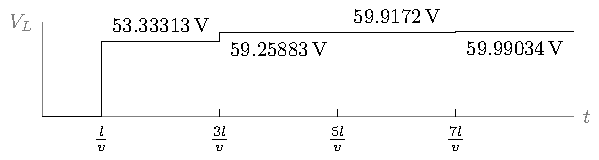
\includegraphics{figTransmissionLineTransientLoadVoltageQuestionB}
\caption{ برقی بوجھ کی برقی دباو بالمقابل وقت۔}
\label{شکل_ترسیلی_جواب_سوال_ب}
\end{subfigure}%

\begin{subfigure}{0.9\textwidth}
\centering
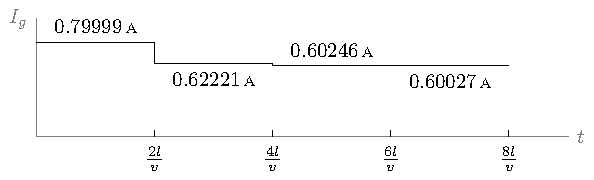
\includegraphics{figTransmissionLineTransientSourceCurrentQuestionB}
\caption{منبع کی برقی رو بالمقابل وقت۔}
\label{شکل_ترسیلی_جواب_منبع_رو_سوال_ب}
\end{subfigure}%
\caption{سوال \حوالہ{سوال_ترسیلی_بار_بردار_ب} کے خط۔}
\label{شکل_سوال_ترسیلی_سوال_ب}
\end{figure}
جواب: شکل \حوالہ{شکل_سوال_ترسیلی_سوال_ب}  میں دکھائے گئے ہیں۔
\انتہا{سوال}
%===========================


\ابتدا{سوال}\شناخت{سوال_ترسیلی_بار_بردار_پ}
صفحہ \حوالہصفحہ{شکل_ترسیلی_عمومی_بار_ابتدائی_موج} میں شکل \حوالہ{شکل_ترسیلی_عمومی_بار_ابتدائی_موج} دکھایا گیا ہے۔اس میں \عددی{Z_0=\SI{50}{\ohm}}،
 \عددی{R_L=\SI{25}{\ohm}}،  \عددی{R_g=\SI{100}{\ohm}} جبکہ منبع کی برقی دباو \عددی{V_0=\SI{10}{\volt}} ہے۔تار کی لمبائی \عددی{\SI{480}{\meter}} ہے جبکہ تار میں موج کی رفتار \عددی{\SI{2.4e8}{\meter\per\second}} ہے۔ لمحہ \عددی{t=0} پر سوئچ چالو کیا جاتا ہے۔\عددی{0<t<\tfrac{8l}{v}} دورانیے کے لئے منبع سے \عددی{\SI{360}{\meter}} فاصلے پر  برقی دباو اور برقی رو کے خط کھینچیں۔

\begin{figure}
\centering
\begin{subfigure}{0.9\textwidth}
\centering
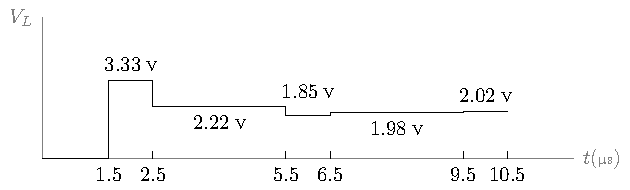
\includegraphics{figTransmissionLineTransientLoadVoltageQuestionC}
\caption{ دئے نقطے کی برقی دباو بالمقابل وقت۔}
\label{شکل_ترسیلی_جواب_سوال_پ}
\end{subfigure}%

\begin{subfigure}{0.9\textwidth}
\centering
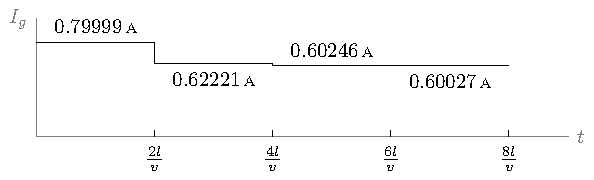
\includegraphics{figTransmissionLineTransientSourceCurrentQuestionB}
\caption{دئے نقطے کی برقی رو بالمقابل وقت۔}
\label{شکل_ترسیلی_جواب_منبع_رو_سوال_پ}
\end{subfigure}%
\caption{سوال \حوالہ{سوال_ترسیلی_بار_بردار_پ} کے خط۔}
\label{شکل_سوال_ترسیلی_سوال_پ}
\end{figure}
جواب: شکل \حوالہ{شکل_سوال_ترسیلی_سوال_پ}  میں دکھائے گئے ہیں۔
\انتہا{سوال}
%===========================
\ابتدا{سوال}\شناخت{سوال_ترسیلی_بار_بردار_ت}
شکل \حوالہ{شکل_ترسیلی_عمومی_بار_ابتدائی_موج}  میں  \عددی{Z_0=\SI{75}{\ohm}}، \عددی{R_g=R_L=\SI{50}{\ohm}} اور \عددی{V_0=\SI{10}{\volt}} ہیں۔لمحہ \عددی{t=0} پر سوئچ چالو کیا جاتا ہے جبکہ لمحہ \عددی{t=\tfrac{l}{4v}} پر سوئچ کو دوبارہ منقطع کر دیا جاتا ہے۔برقی بوجھ پر برقی دباو کا خط \عددی{0<t<\tfrac{8l}{v}} دورانیے کے لئے کھینچیں۔
\begin{figure}
\centering
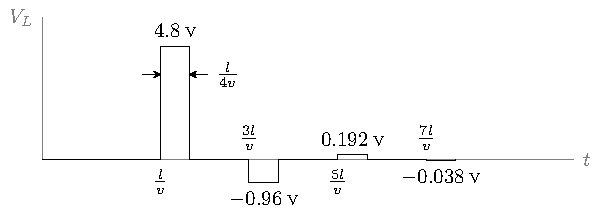
\includegraphics{figTransmissionLineTransientLoadVoltageQuestionD}
\caption{سوال \حوالہ{سوال_ترسیلی_بار_بردار_ت} میں برقی بوجھ پر مستطیل برقی دباو۔}
\label{شکل_ترسیلی_سوال_مستطیل_دباو}
\end{figure}

جواب:سوئچ چالو کرنے سے \عددی{V_1^+=\SI{6}{\volt}} اور \عددی{I_1^+=\SI{0.08}{\ampere}} امواج پیدا ہوتی ہیں۔سوئچ منقطع کرنے سے برقی رو صفر ہو جاتی ہے۔جس کا مطلب ہے کہ اب \عددی{I_1^{'+}=\SI{-0.08}{\ampere}} کی موج پیدا ہوئی ہے یعنی برقی دباو کی موج \عددی{V_1^{'+}=\SI{-6}{\volt}} کی موج پیدا ہوئی ہے۔برقی دباو کی دونوں امواج مل کر مستطیل موج کو جنم دیتی ہیں۔شکل \حوالہ{شکل_ترسیلی_سوال_مستطیل_دباو} میں نتائج دکھائے گئے ہیں۔
\انتہا{سوال}
%=========================
